
\documentclass[
   ngerman          % neue deutsche Rechtschreibung
  ,a4paper          % Papiergrösse
% ,twoside          % Zweiseitiger Druck (rechts/links)
% ,10pt             % Schriftgrösse
% ,11pt
 ,12pt
  ,pdftex
  ,disable         % Todo-Markierungen auschalten
%  ,ngerman
]{scrreprt}

%\usepackage{subcaption}
\usepackage[onehalfspacing]{setspace} %Zeilenabstand
%\usepackage[doublespacing]{setspace} %Zeilenabstand

% Bitte die Codierung Ihrer Dateien auswählen:
% \usepackage[latin1]{inputenc}    % Für UNIX mit ISO-LATIN-codierten Dateien
 \usepackage[applemac]{inputenc}  % Für Apple Mac
% \usepackage[ansinew]{inputenc}   % Für Microsoft Windows
%\usepackage[utf8]{inputenc}        % UTF-8 codierte Dateien
                                   % Dieses Dokument ist unter Unix erstellt, daher
                                   % wird diese Input-Codierung benutzt.
\usepackage{booktabs}
\usepackage{array,multicol,booktabs,tabularx}
\usepackage{graphicx}
\usepackage{bericht}
\usepackage[german,english]{babel}
%\selectlanguage{english}
\usepackage{amsmath,esint}
\usepackage[binary-units = true]{siunitx}
\sisetup{
  locale = DE ,
  per-mode = symbol
}
\DeclareSIUnit{\sqrthz}{\ensuremath{\sqrt{\text{\hertz}}}}
\DeclareSIUnit{\voltnoise}{\volt\per\sqrthz}
\DeclareSIUnit{\decibelm}{\ensuremath{\text{dBm}}}
\DeclareSIUnit{\decibeli}{\ensuremath{\text{dBi}}}
\usepackage{textcomp}
\usepackage{xfrac}
\usepackage{extarrows}
\usepackage{xspace}
\usepackage{listings}
\lstset{basicstyle=\ttfamily,
  showstringspaces=false,
  commentstyle=\color{red},
  keywordstyle=\color{blue}
}
\usepackage{enumitem}

\graphicspath{{./Images/}} %Setting the graphicspath
% ============= Dokumentinformationen =======================================

%\newcommand{\Bericht}{Laborbericht}
\newcommand{\Titel}{Master Thesis}
\newcommand{\Was}{Measurement uncertainty assessment for novel approach of wireless co-existence testing}
\newcommand{\WasEng}{}
\newcommand{\Referent}{Prof. Dr.-Ing. S. Peik}
\newcommand{\Korreferent}{}
\newcommand{\Betreuer}{MSc. Johannes Koebele}
\newcommand{\Autor}{Mrinal Shinde}
\newcommand{\UNI}{Hochschule Bremen}
\newcommand{\Studiengang}{Faculty for Electrical Engineering and Computer Science}
\newcommand{\MatrikelNummer}{5021349}
\newcommand{\Zeitraum}{18.11.2019 - 18.07.2020}
% Wird auf dem Deckblatt in der Erklärung benutzt

\newcommand{\abs}[1]{\ensuremath{\left\vert#1\right\vert}}

%%%%%%%%%%%%%%%%%%%%%%%%%%%%%%%%%%%%%%%%%%%%%%%%%%%%%%%%%%%%%%%%%%%%%%%%%%%%%%%%%%%%%

\hypersetup{%%
  pdfauthor={\Autor},
  pdftitle={\Titel},
  pdfsubject={\Was}
}

%%%%%%%%%%%%%%%%%%%%%%%%%%%%%%%%%%%%%%%%%%%%%%%%%%%%%%%%%%%%%%%%%%%%%%%%%%%%%%%

% Wenn \includeonly{..} benutzt wird, werden nur diese Kaptitel ausgegeben.
%\includeonly{
%  abk
% ,adaption
%}

%%%%%%%%%%%%%%%%%%%%%%%%%%%%%%%%%%%%%%%%%%%%%%%%%%%%%%%%%%%%%%%%%%%%%%%%%%%%%%%

% Benutzt man das "biblatex"-Paket, dann muß das hier stehen:
% siehe auch die mit BIBLATEX markierten Zeilen in bericht.sty
\bibliography{literatur}

\begin{document}
%%%%%%%%%%%%%%%%%%%%%%%%%%%%%%%%%%%%%%%%%%%%%%%%%%%%%%%%%%%%%%%%%%%%%%%%%%%%%%%
\pagenumbering{roman}

\begin{titlepage}

\begin{singlespace}
\begin{center}
\begin{singlespace}
\Large \Titel\\[1.2cm]
\end{singlespace}
\begin{spacing}{2}
{\Huge\scshape \Was}\\
{\Large \WasEng}\\[0.6cm]
\end{spacing}
\end{center}
\end{singlespace}

\begin{flushleft}
	\begin{center}
		
\includegraphics[width=12cm]{HSKA_Logo_Hska_Logo.pdf}
		%\includegraphics[width=12.7cm]{8_2_3_3_Bild1.JPG}
	\end{center}
\end{flushleft}

\begin{singlespace}
\begin{center}
%\vspace*{-2cm}
{\large \Studiengang}\\[0.5cm]
{\large von}\\[0.5cm]
{\large\bfseries \Autor}\\[0.5cm]
\vfill
\end{center}
\begin{tabular}{l@{\hspace{2cm}}l}
Matrikelnummer	                 & \MatrikelNummer		\\
Thesis Nummer		& \ThesisNummer \\
Zeitraum	&	\Zeitraum \\ \\
Referent der Hochschule	 & \Referent		\\
Korreferent der Hochschule	 & \Korreferent		\\ \\
Betreuer am Arbeitsplatz	 & \Betreuer		\\
Firma	 & \firma		\\
\end{tabular}
\end{singlespace}
\end{titlepage}


%\vspace{0cm}

%\begin{center}
%
%	\Huge{
%		\textbf{\Vorlesung}} \\[0.5cm]
%	\huge{
%		\textbf{{\Versuch}}\\[7.0cm]
%		}
%	\normalsize{
%		}
%	\normalsize{
%		\textbf{{\Versuchstermin}}\\[3.0cm]
%	}
%	
%	\small{
%		\textbf{\firma} \\
%	}
 %   \small{
	%	\textbf{\studiengang} \\
	%	}
	

%\end{center}
%
%}



%%%%%%%%%%%%%%%%%%%%%%%%%%%%%%%%%%%%%%%%%%%%%%%%%%%%%%%%%%%%%%%%%%%%%%%%%%%%%%%

% Nur für Bachelorarbeiten einfügen:
\setlength{\parindent}{0pt}


\newpage
\thispagestyle{empty}
%\begin{framed}
\begin{center}
\Huge\emph{Abstract}
\end{center}
\medskip
\noindent

You schould measure \ac{RSE} to be sure of not disturbing others!
 
%%%%%%%%%%%%%%%%%%%%%%%%%%%%%%%%%%%%%%%%%%%%%%%%%%%%%%%%%%%%%%%%%%%%%%%%%%%%%%%
%% Descr:       Vorlage für Berichte der DHBW-Karlsruhe, Erklärung
%% Author:      Prof. Dr. Jürgen Vollmer, vollmer@dhbw-karlsruhe.de
%% $Id: erklaerung.tex,v 1.6 2016/03/16 12:51:09 vollmer Exp $
%% -*- coding: utf-8 -*-
%%%%%%%%%%%%%%%%%%%%%%%%%%%%%%%%%%%%%%%%%%%%%%%%%%%%%%%%%%%%%%%%%%%%%%%%%%%%%%%

% In Bachelorarbeiten muss eine schriftliche Erklärung abgegeben werden.
% Hierin bestätigen die Studierenden, dass die Bachelorarbeit, etc.
% selbständig verfasst und sämtliche Quellen und Hilfsmittel angegeben sind. Diese Erklärung
% bildet das zweite Blatt der Arbeit. Der Text dieser Erklärung muss auf einer separaten Seite
% wie unten angegeben lauten.

\newpage
\thispagestyle{empty}
%\begin{framed}
\begin{center}
\Huge\emph{Eidesstattliche Erklärung}
\end{center}
\medskip
\noindent
Ich versichere hiermit, dass ich meine \Titel\ mit
dem Thema: \glqq \Was \grqq{ }selbständig verfasst und keine anderen als die angegebenen Quellen und Hilfsmittel benutzt habe.

\vspace{3cm}
\noindent
\underline{\hspace{6cm}}\hfill\underline{\hspace{6cm}}\\
Ort\hspace{2.5cm}Datum\hfill Unterschrift\hspace{3.8cm}
%\end{framed}

\vfill
%\emph{Sofern von der Ausbildungsstätte ein Sperrvermerk gewünscht %wird, ist folgende Formulierung
%zu verwenden:}
%\begin{framed}
%\begin{center}
%\Large\bfseries Sperrvermerk
%\end{center}
%\medskip
%\noindent
%Der Inhalt dieser Arbeit darf weder als Ganzes noch in Auszügen %Personen
%auerhalb des Prüfungsprozesses und des Evaluationsverfahrens %zugänglich gemacht
%werden, sofern keine anders lautende Genehmigung der %Ausbildungsstätte vorliegt.
%\end{framed}

%%%%%%%%%%%%%%%%%%%%%%%%%%%%%%%%%%%%%%%%%%%%%%%%%%%%%%%%%%%%%%%%%%%%%%%%%%%%%%%
\endinput
%%%%%%%%%%%%%%%%%%%%%%%%%%%%%%%%%%%%%%%%%%%%%%%%%%%%%%%%%%%%%%%%%%%%%%%%%%%%%%%
 %declaration


\newpage
\thispagestyle{empty}
%\begin{framed}
\begin{center}
\Huge\emph{Vorwort}
\end{center}
\medskip
\noindent

Hier möchte ich allen danken, die mich bei dieser Arbeit fachlich und persönlich unterstützt haben. Mein besonderer Dank gilt meinem Betreuer bei Rohde \& Schwarz in München Heinz Mellein, der das interessante Thema bereitstellte und mich bei der Durchführung immer sehr freundlich, kompetent und unkompliziert betreut hat. Außerdem möchte ich meinen Kollegen Johannes Köbele und Gerhard Hamberger danken, ohne deren gute Ratschläge und allgemeine Unterstützung diese Arbeit in dieser Form nicht möglich gewesen wäre. Ich möchte auch Ahmed Ezzouhri und Simon Lachner für die Unterstützung bei langwierigen Messkampagnen danken. Auch danke ich meinen betreuenden Professoren der Hochschule Karlsruhe Manfred Litzenburger und Hans Sapotta für ihre zurückhaltende, freundliche und kompetente Unterstützung. Vor allem danke ich der Kantine von Rohde und Schwarz für die gute und günstige Verpflegung und allen neuen Freunden in München für die tolle und abwechslungsreiche Zeit hier.

\begin{flushright}
Fabian Michaelsen\\
September 2019\\
München
\end{flushright}
 %preamble

\tableofcontents           % Inhaltsverzeichnis hier ausgeben
\listoffigures             % Liste der Abbildungen
\listoftables              % Liste der Tabellen
%\lstlistoflistings         % Liste der Listings
%\listofequations           % Liste der Formeln
% Jetzt kommt der "eigentliche" Text
%%%%%%%%%%%%%%%%%%%%%%%%%%%%%%%%%%%%%%%%%%%%%%%%%%%%%%%%%%%%%%%%%%%%%%%%%%%%%%
%% Descr:       Vorlage für Berichte der DHBW-Karlsruhe, Datei mit Abkürzungen
%% Author:      Prof. Dr. Jürgen Vollmer, vollmer@dhbw-karlsruhe.de
%% $Id: abk.tex,v 1.3 2016/03/16 12:21:40 vollmer draft $
%% -*- coding: utf-8 -*-
%%%%%%%%%%%%%%%%%%%%%%%%%%%%%%%%%%%%%%%%%%%%%%%%%%%%%%%%%%%%%%%%%%%%%%%%%%%%%%%

\chapter*{List of Abbreviations}                   % chapter*{..} -->   keine Nummer, kein "Kapitel"
						         % Nicht ins Inhaltsverzeichnis
% \addcontentsline{toc}{chapter}{Akürzungsverzeichnis}   % Damit das doch ins Inhaltsverzeichnis kommt

% Hier werden die Abkürzungen definiert
\begin{acronym}[FIAFTA]
  % \acro{Name}{Darstellung der Abkürzung}{Langform der Abkürzung}
 \acro{Abk}[Abk.]{Abkürzung}

 % Folgendes benutzen, wenn der Plural einer Abk. benöigt wird
 % \newacroplural{Name}{Darstellung der Abkürzung}{Langform der Abkürzung}
 \newacroplural{Abk}[Abk-en]{Abkürzungen}

 \acro{H2O}[\ensuremath{H_2O}]{Di-Hydrog-Monoxid}

 % Wenn neicht benutzt, erscheint diese Abk. nicht in der Liste
 \acro{NUA}{Not Used Acronym}
 
 \acro{3GPP}{3rd Generation Partnership Project}
 \acro{5G}{Fifth Generation mobile communication}
 \acro{AAS}{Active Antenna System}
 \acro{AC}{Anechoic Chamber}
 \acro{ANSI}{American National Standards Institute}
 \acro{ATS}{Antenna Test System}
 \acro{CATR}{Compact Antenna Test Range}
 \acro{CC}{Clenshaw–Curtis}
 \acro{CDG}{Constant Density Grid}
 \acro{CEPT}{European Conference of Postal and Telecommunications Administrations}
 \acro{CrefA}{Correction Factor Reference Angle}
 \acro{CSSG}{Constant Step Size Grid}
 \acro{DANL}{Displayed Average Noise Level}
 \acro{DUT}{Device Under Test} 
 \acro{EBW}{Emission Bandwidth}
 \acro{EIRP}{Equivalent Isotropic Radiated Power}
 \acro{EM}{Electro Magnetic}
 \acro{EMC}{Electro Magnetic Compatibility}
 \acro{ETSI}{European Telecommunications Standards Institute}
 \acro{EU}{European Union}
 \acro{FCC}{Federal Communications Commission}
 \acro{FF}{Far-Field}
 \acro{FFT}{Fast Fourier Transformation}
 \acro{FR2}{Frequency Range two}
 \acro{FSPL}{Free Space Path Loss}
 \acro{IEEE}{Institute of Electrical and Electronics Engineers}
 \acro{ITU}{International Telecommunication Union}
 \acro{LB}{Link Budget}
 \acro{MIMO}{Multiple In Multiple Out}
 \acro{mmW}{milli-meter Wave}
 \acro{NF}{Near-Field}
 \acro{NR}{New Radio}
 \acro{OATS}{Open Area Test Site}
 \acro{OBW}{Occupied Bandwidth}
 \acro{OEM}{Original Equipment Manufacturer}
 \newacroplural{OEM}[OEMs]{Original Equipment Manufacturer}
 \acro{OOBE}{Out Of Band Emission}
 \acro{OTA}{Over The Air}
 \acro{PM}{Pattern Multiplication}
 \acro{QZ}{Quiet zone}
 \acro{RBW}{Resolution Bandwidth}
 \acro{RF}{Radio Frequency}
 \acro{RMS}{Root Mean Square}
 \acro{RS}[R\&{}S]{Rohde \& Schwarz GmbH \& Co. KG}
 \acro{RSE}{Radiated Spurious Emission} 
 \acro{RVC}{Reverberation Chamber}
 \acro{SE}{Spurious Emission}
 \acro{SF}{Sparsity Factor}
 \acro{SGH}{Standard Gain Horn}
 \acro{TMP}{Total Measurement Power}
 \acro{TRP}{Total Radiated Power}
 \acro{TSP}{Travelling Salesman Problem}
 \acro{UE}{User Equipment}
 \acro{UnE}{Unwanted Emission}
 \acro{USA}{United States of America}
 \acro{VNA}{Vector Network Analyzers}
 \acro{VSG}{Vector Signal Generator}


\end{acronym}              
\pagenumbering{arabic}

%% uncocmment these
\chapter{Introduction}

In this chapter the motivation and aim of this work is phrased. Furthermore the current emission limits and the necessary terms are presented.

\section{Motivation}

\ac{3GPP} \ac{5G} is occupying \acp{mmW} in \ac{FR2} with frequencies $\ge\SI{28}{\giga\hertz}$ \cite{trp}. With this development big and highly integrated  \acp{AAS} will be needed. That makes the conducted conformance test approach with antenna connectors in the \ac{UE} impossible. The equivalent metric to conducted measurements for \ac{RSE} is now \ac{TRP} and the measurement is carried out \ac{OTA}.

%Higher frequencies imply shorter wavelengths. Multi-antenna arrays at mmWave frequencies will help overcome signal propagation issues and deliver directional antennas with higher gain. With shorter wavelengths, antenna elements can be spaced more tightly, resulting in extremely compact arrays. Many vendors even opt to develop arrays that integrate into ICs. Of course, highly integrated ICs have no place to probe and no place to put connectors. A consequence of this integration is it has become impractical to use traditional RF connectors between the radio circuit and the antenna, bringing the need for OTA tests. https://www.testandmeasurementtips.com/why-5g-is-going-to-over-the-air-testing-faq/

\section{Aim}

The aim of this work is to find an optimal solution for conformance  \ac{TRP}-measurements using \acp{AC}. In dependence of the dimension of the \ac{DUT} an ideal grid and measurement distance for a wanted precision shall be found. To achieve that, theoretical knowledge shall be projected on simulations and the outcome shall be proofed in real measurements.

\section{Legal Emission Limits}
\label{sec:legem}

In this section the official \ac{EM} emission limits are acknowledged by the example of the regulation in the \ac{USA} and the \ac{EU}. The \ac{ITU} provides a recommendation \cite{seitur} about the emission limits for the national regulators. These regulators, in the \ac{EU} the \ac{CEPT} and in the \ac{USA} the \ac{FCC}, publish with the help of dedicated standardisation organisations, e.g. \ac{ETSI} (\ac{EU}), \ac{ANSI} (\ac{USA}) or other \acp{SDO}, limits which become law; \cite{ceptercrec}, \cite{ansi}. The \ac{3GPP}, the \ac{IEEE} or other \acp{SDO} develop a new telecommunication standard and adopt to this laws.\\
To quantify emission limits the following terms are declared regarding \cite{seitur} and \cite{ctiaat}:

\begin{itemize}
\item An \textbf{\acf{UnE}} consists of \ac{SE} and \ac{OOBE}.
\item A \textbf{\acf{SE}} is an emission on a frequency, or frequencies, which are outside the necessary bandwidth and the level of which may be reduced without affecting the corresponding transmission of information. \acl{SE} include harmonic
emissions, parasitic emissions, intermodulation products and frequency conversion products but exclude \ac{OOBE}.
\item An \textbf{\acf{OOBE}} is an emission on a frequency or frequencies immediately outside the necessary bandwidth which results from the modulation process, excluding \aclp{SE}.
\item The \textbf{\acf{OBW}} is the bandwidth wherein $\SI{99}{\percent}$ of the power is radiated.
\item The \textbf{\acf{EBW}} is used by the \ac{FCC} and describes a bandwidth which is surrendered out of that tow points in the spectra lying $\SI{26}{\decibel}$ under the power of the \ac{OBW}. 
\item \textbf{\acf{TRP}} is the \ac{OTA} equivalent for measuring connected and describes all power radiated by a device. It is the average spherical \ac{EIRP}.
\end{itemize}


In table \ref{tab:legusa} the emission limits from \cite{ceptercrec}, \cite{ansi} and \cite{fcc} are summarized. The used terms are illustrated in fig. \ref{fig:sem}.

\begin{table}
\centering
\caption{Legal Emission Limits}
\label{tab:legusa}
\begin{tabular}{|c|c|c|c|}
\hline
$f_c$  &  $f_l$ & $f_h$ & $p_e$ \\\hline
\multicolumn{4}{|c|}{\textbf{USA}} \\\hline
$\SI{9}{\kilo\hertz}-\SI{10}{\giga\hertz}$ & $\SI{9}{\kilo\hertz}$ & $10f_c\ \text{or}\ \SI{40}{\giga\hertz}$ & $\SI{-13}{\decibelm\per\mega\hertz}$ \\\hline
$\SI{10}{\giga\hertz}-\SI{30}{\giga\hertz}$ & $\SI{9}{\kilo\hertz}$ & $5f_c\ \text{or}\ \SI{100}{\giga\hertz}$ & $\SI{-13}{\decibelm\per\mega\hertz}\ \text{or}\ 1\% \text{EBW}$ \\\hline
$\SI{30}{\giga\hertz}-\dots$ & $\SI{9}{\kilo\hertz}$ & $5f_c\ \text{or}\ \SI{200}{\giga\hertz}$ & $\SI{-13}{\decibelm\per\mega\hertz}\ \text{or}\ 1\% \text{EBW}$ \\\hline
\multicolumn{4}{|c|}{\textbf{EU}} \\\hline
$\SI{9}{\kilo\hertz}-\SI{100}{\mega\hertz}$ & $\SI{9}{\kilo\hertz}$ & $\SI{1}{\giga\hertz}$ & $\SI{-36}{\decibelm\per \SI{100}{\kilo\hertz}}$ \\\hline
$\SI{100}{\mega\hertz}-\SI{300}{\mega\hertz}$ & $\SI{9}{\kilo\hertz}$ & $10f_c$ & $\SI{-36}{\decibelm\per \SI{100}{\kilo\hertz}}$ \\\hline
$\SI{300}{\mega\hertz}-\SI{600}{\mega\hertz}$ & $\SI{30}{\mega\hertz}$ & $\SI{3}{\giga\hertz}$ & $\SI{-36}{\decibelm\per \SI{100}{\kilo\hertz}}$ \\\hline
$\SI{600}{\mega\hertz}-\SI{1}{\giga\hertz}$ & $\SI{30}{\mega\hertz}$ & $5f_c$ & $\SI{-36}{\decibelm\per \SI{100}{\kilo\hertz}}$ \\\hline
$\SI{1}{\giga\hertz}-\SI{5.2}{\giga\hertz}$ & $\SI{30}{\mega\hertz}$ & $5f_c$ & $\SI{-30}{\decibelm\per\mega\hertz}$ \\\hline
$\SI{5.2}{\giga\hertz}-\SI{7.25}{\giga\hertz}$ & $\SI{30}{\mega\hertz}$ & $\SI{26}{\giga\hertz}$ & $\SI{-30}{\decibelm\per\mega\hertz}$ \\\hline
$\SI{7.25}{\giga\hertz}-\dots$ & $\SI{30}{\mega\hertz}$ & $2f_c$ & $\SI{-13}{\decibelm\per\mega\hertz}\ \text{and}\ \SI{-10}{\decibelm\per \SI{100}{\kilo\hertz}}$ \\\hline
\end{tabular}
\end{table}

\begin{figure}
\centering
\def\svgwidth{0.9\textwidth}
\input{Bilder/EmissionMask.pdf_tex}
\caption{Spurious Emissions Mask}
\label{fig:sem}
\end{figure}









\chapter{Theoretical Background}

This chapter will give a brief overview about the underlying theoretical background in the fields of antenna theory, spatial sampling, will introduce quadrature methods for deriving the \ac{TRP} out of spherical \ac{EIRP} data and will establish the needed stochastic for the used statistic.

\section{Antenna Field Regions}

\begin{figure}[H]
\centering
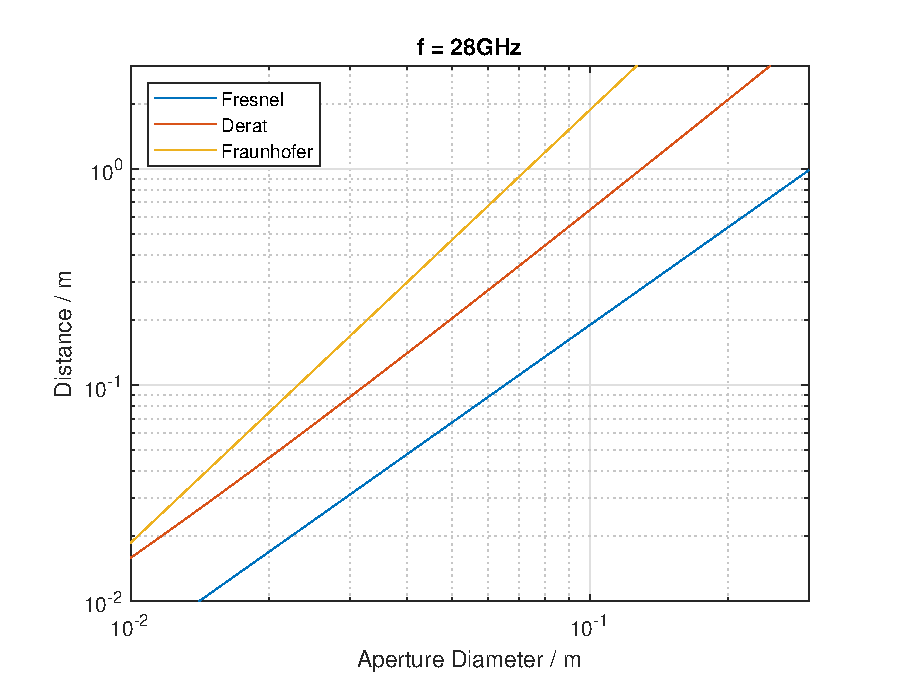
\includegraphics[width=0.6\textwidth]{Matlab/AntennaFieldRegions.eps}
\caption{Antenna field regions overview}
\label{fig:antennafieldreg}
\end{figure}

There are three commonly known antenna field regions, the reactive \ac{NF}, the radiating \ac{NF} and the \ac{FF}, divided by two boundaries, the Fresnel distance (blue) and the Fraunhofer distance (yellow). These distances are shown in figure \ref{fig:antennafieldreg}, where the aperture diameter of an arbitrary antenna is on the x-axis and the distance form it is on the y-axis. The third line, the Derat distance (red), was introduced by Benoit Derat in \cite{8393926}.\\
\ac{FF}-distance and \ac{NF}-distance are derivable from the phase fluctuation due to the maximum diameter of the antennas aperture \cite{7942128} in a distance $r$ from the antennas phase center. The phase fluctuation is given by the different length of $r$ and $R$, as you can see in figure \ref{fig:arbaperturexy}. The maximum runtime difference is found at the minimum radius of the circle enclosing the aperture at $\sfrac{D}{2}$. The field boundaries are derived from the Taylor series of the function of the phase in dot $P$. Fresnel and Fraunhofer distance, the boundaries between reactive \ac{NF}, radiating \ac{NF} (Fresnel-Region) and the \ac{FF} (Fraunhofer-Region), are analogue to their optical counterpart. \cite{7942128} \cite{balanis}

\begin{figure}[H]
\centering
\def\svgwidth{0.6\textwidth}
\input{Bilder/AntennaApature.pdf_tex}
\caption{An arbitrary radiating aperture in the $yz$ plane. \cite{7942128}}
\label{fig:arbaperturexy}
\end{figure}

$R$ is the distance from an arbitrary point on the aperture to an other arbitrary point $P$ in the volume. With $r$, the distance from the phase center of the antenna to the point $P$, $R$ can be written as: \cite{balanis}

\begin{equation}
R = \sqrt{\left(x^2+y^2+z^2\right)-\left(2zz'-z^{\prime\, 2}\right)}=\sqrt{r^2-\left(2rz'\sin \theta -z^{\prime\, 2}\right)}
\end{equation}

Using the binomial expansion, $R$ can then be rewritten as:

\begin{equation}
R = r - z'\sin\theta + \frac{1}{r}\left(\frac{z^{\prime\, 2}}{2}\cos ^2 \theta\right) + \frac{1}{r^2}\left(\frac{z^{\prime\, 3}}{2}\sin\theta\cos^2\theta\right) + \dots
\end{equation}

\subsection{Far-Field}

According to \cite{balanis} the \ac{FF}-distance is \glqq that region of the field of an antenna where the angular field distribution is essentially independent of the distance from the antenna.\grqq{ }That means that the antenna's pattern is mostly independent from the distance to the antenna.\\
For the \ac{FF} assumption it is convenient to use the two most significant terms of the binomial expansion $R\approx r - z'\sin\theta$. Hence the error of that truncation can be expressed as the maximum of the third most significant term:

\begin{equation}
\frac{1}{r}\left(\frac{z^{\prime\, 2}}{2}\cos ^2 \theta\right)_\text{max} = \frac{z^{\prime\, 2}}{2r} \quad , \quad \theta = 0
\label{eq:dphi1}
\end{equation}

Introducing the angular wavenumber $k=\sfrac{2\pi}{\lambda}$ and $z'=\sfrac{D}{2}$, formula \ref{eq:dphi1} can be written as:


\begin{equation}
\Delta\theta = \frac{k\cdot z^{\prime\, 2}}{2r} =\frac{\frac{2\pi}{\lambda}\cdot \left(\frac{D}{2}\right)^2}{2r} = \frac{\pi D^2}{4\lambda\cdot r}
\end{equation}

With the typically tolerated phase error of $\Delta\theta = \sfrac{\pi}{8} \ \widehat{=}\  22.5^\circ$ the well known \ac{FF}-distance-formula $r_{\text{FF}}$ can be derived:

\begin{equation}
\frac{\pi}{8} = \frac{\pi D^2}{4\lambda\cdot r_{\text{FF}}} \quad \Leftrightarrow \quad r_{\text{FF}} = \frac{2D^2}{\lambda}
\label{eq:ff}
\end{equation}

This equation is valid for $D > \lambda$. \cite{balanis}

\subsection{Near-Field}

The radiating \ac{NF} (Fresnel) -region is defined by \cite{balanis} as \glqq that region of the field of an antenna between the reactive near-field region and the far-field region wherein radiation fields predominate and wherein the angular field distribution is dependent upon the distance from the antenna.\grqq{ }That means that the antennas pattern is dependent from the distance to the antenna.\\
In the radiating \ac{NF} the deviation from the third most significant term is more then $\sfrac{\pi}{8}$, so it is no longer negligible. With the derivation of the next term the maximum deviation is found:

\begin{align}
\frac{\partial}{\partial\theta}\left(\frac{1}{r^2}\left(\frac{z^{\prime\, 3}}{2}\sin\theta\cos^2\theta\right)\right) = \frac{z^{\prime\, 3}}{2r^2}\cos\theta\left(\cos^2\theta-2\sin^2\theta\right) = 0 \quad \Leftrightarrow\\ 
\theta_1 = \frac{\pi}{2},\ \theta_2=2\arctan\left(\sqrt{5-2\sqrt{6}}\right) \quad \Leftrightarrow
\end{align}

By introducing the angular wavenumber $k=\sfrac{2\pi}{\lambda}$, the minimum sphere diameter $D$, so that $z'=\sfrac{D}{2}$ and the phase error of $\Delta\phi = \sfrac{\pi}{8} \ \widehat{=}\  22.5^\circ$ the \ac{NF} (Fresnel)-distance-formula $r_{\text{NF}}$ can be derived:

\begin{equation}
\Delta\phi = \frac{\pi}{8} = \frac{kz^{\prime\, 3}}{2r_{\text{NF}}^2}\sin\theta_2\cos^2\theta_2= \frac{\pi D^3}{12\sqrt{3}\cdot\lambda r_{\text{NF}}^2} \quad \Leftrightarrow \quad r_{\text{NF}}=0.62\sqrt{\frac{D^3}{\lambda}}
\end{equation}

The region directly surrounding the antenna in front of this boundary is called reactive \ac{NF} and it is according to \cite{balanis} \glqq that portion of the near-field region immediately surrounding the antenna wherein the reactive field predominates.\grqq{ }In other words, the reactive \ac{NF} is that portion of an antennas field were direct coupling is expected.

\subsection{Derat Distance}

The Derat distance was introduced by Benoit Derat in \cite{8393926} and it is that distance, in which the main beam of an antenna is in \ac{FF} condition. For the understanding of the Derat distance $r_{\text{Dr}}$ other considerations need to take place: It is about spherical modes described by spherical Hankel functions  of the second kind. \cite{8393926} \cite{hansen}\\
In \cite{8393926} it is shown, that higher order modes than 

\begin{equation}
N = \Bigg\lceil 1.0252\cdot\left(\frac{\pi D}{\lambda}\right)^{0.8633} \Bigg\rceil
\end{equation}

have a maximum influence to the \ac{EIRP} in main direction of $\SI{0.5}{\decibel}$. $\lceil\cdot\rceil$ means rounding up. With that the Derat distance can be derived to:

\begin{equation}
r_{\text{Dr}} = \lambda\left(\frac{\pi D}{\lambda}\right)^{0.8633}\cdot\left(0.1673\left(\frac{\pi D}{\lambda}\right)^{0.8633}+0.1632\right)
\end{equation}

\subsection{Example: Standard Gain Horn}

\begin{figure}[h]
\centering
  \centering
  \subfigure[Wave impedance]{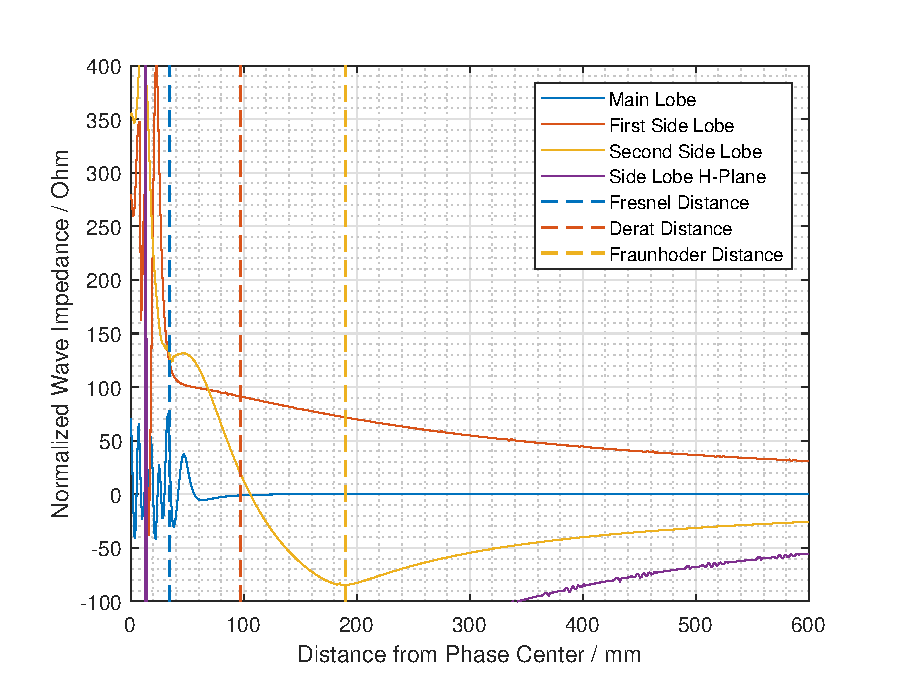
\includegraphics[width=0.49\textwidth]{Matlab/NormWaveImpHorn.eps}}
  \centering
  \subfigure[Phase]{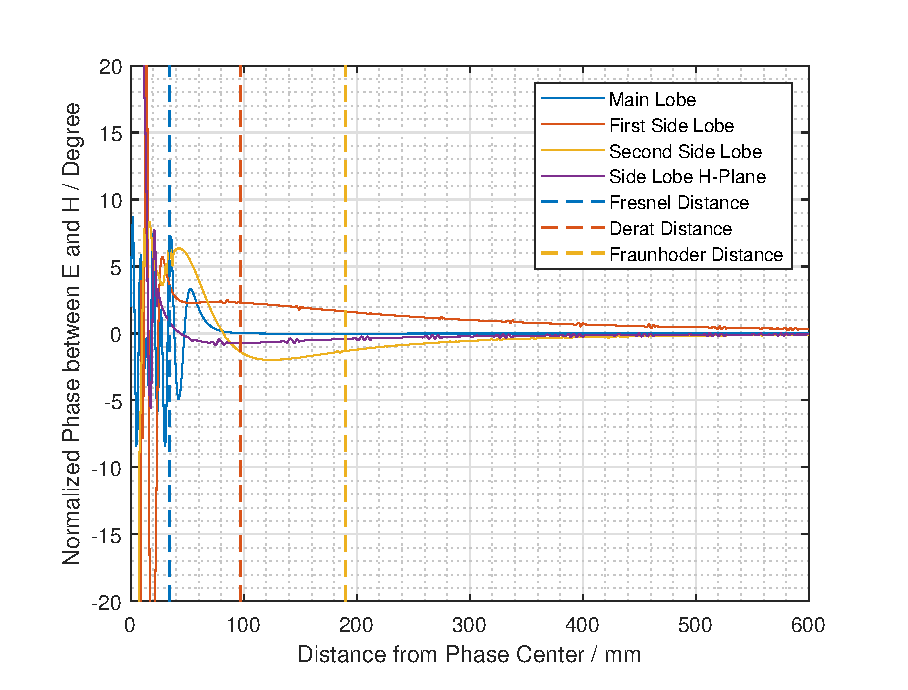
\includegraphics[width=0.49\textwidth]{Matlab/NormPhaseHorn.eps}}
  \centering
  \subfigure[EIRP]{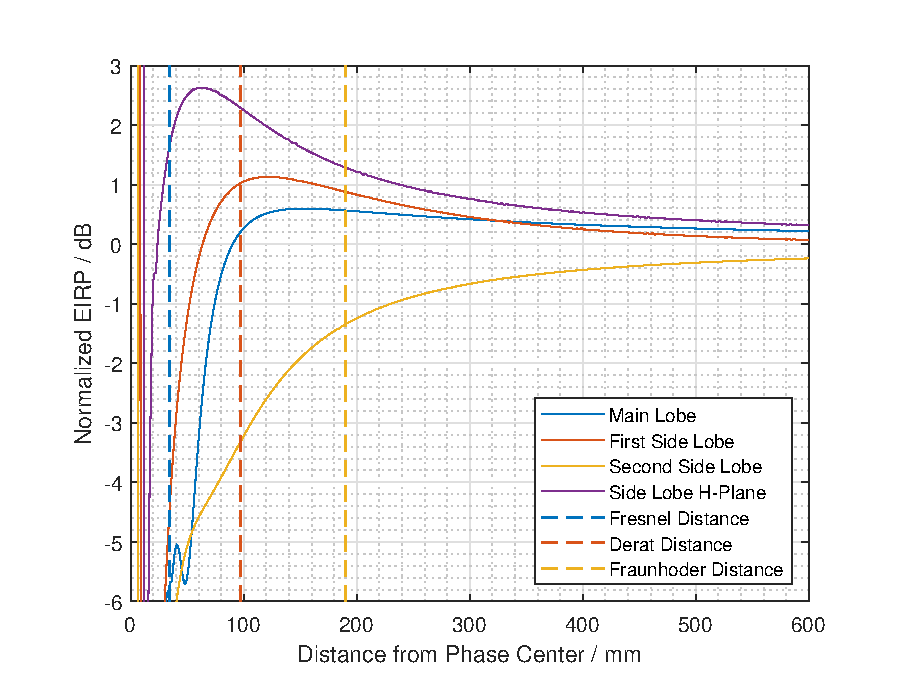
\includegraphics[width=0.49\textwidth]{Matlab/NormEIRPHorn.eps}}
  \centering
  \subfigure[Antenna Pattern E-Plane]{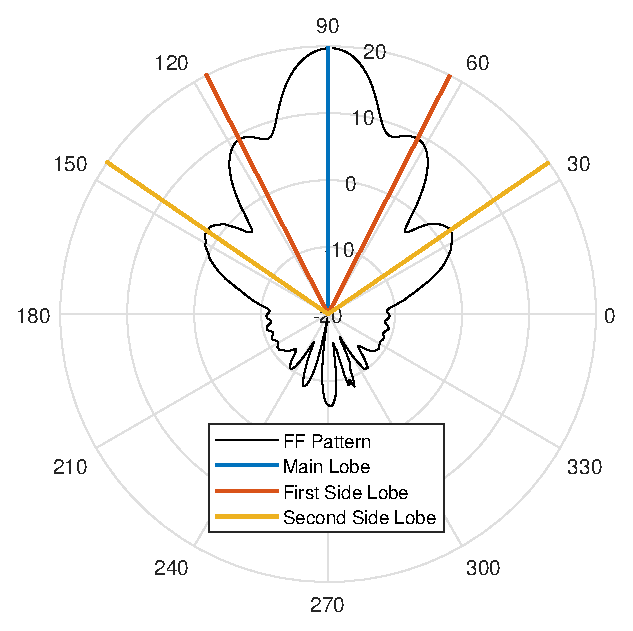
\includegraphics[width=0.35\textwidth]{Matlab/ePlanePattern.eps}}
\caption{Beam comparison of a $\SI{20}{\decibel}$ SGH at $\SI{28}{\giga\hertz}$}
\label{fig:beamcpmp}
\end{figure}

To clarify the introduced distances they will be proved based on a $\SI{20}{\decibel}$ \ac{SGH} at $\SI{28}{\giga\hertz}$. The front view of this horn with the underlying field distribution is plotted in figure \ref{fig:fielddist} in the annex. The polarisation is in $y$-direction, so the $yz$-plane is called E-plane and the $xz$-plane is called H-plane from here on.\\
In figure \ref{fig:beamcpmp} the normalized wave impedance (a), the normalized phase between E- and H-field components (b) and the normalized \ac{EIRP} (c) over the distance to the phase center are plotted. To clarify the designations the directions are plotted in (d). The data have been generated by CST\texttrademark , a full wave simulation tool. Complex data in $x$, $y$, and $z$ direction was exported and post processed to Matlab\texttrademark{}.\\
Also the field boundaries from the sections above are plotted with dashed lines. For the derivation of the field boundaries only the opening of the horn in the E-plane was taken to account. This is sensible because the field distribution and thus the usage of the aperture is known, refer to figure \ref{fig:fielddist}. As it can be seen, in the E-plane the aperture is fully used. But if the field distribution is unknown, the smallest circle enclosing the aperture has to be taken.\\
The main lobe (blue line) is from Derat-distance on in \ac{FF} condition. The wave impedance reached its end value of $120\pi\si{\ohm}\approx\SI{377}{\ohm}$, E- and H-fields are coherent and the \ac{EIRP} value converged. Considering the side lobes it can be seen that in the reactive \ac{NF} the field conditions are very unstable, whereas the fields in the radiating \ac{NF} become more stable. In the \ac{FF} the field values are continually decreasing the offset from their final value.\\
In figure \ref{fig:devantennap} in the annex the resulting antenna patterns in different radii are depicted as well in Cartesian coordinates (a) as in Polar coordinates (b). The assumption 

\begin{equation}
S = \frac{E^2}{Z_0}
\label{eq:poynting}
\end{equation}

was taken to account. In addition analogue to (a) and (b) in (c) the \ac{EIRP} computed in different radii is plotted in figure \ref{fig:fielddist}. At Derat distance ($\approx\SI{100}{\milli\meter}$) the error in main beam direction is about $\SI{0.5}{\decibel}$ and the antenna pattern is further evolving after the Fraunhofer distance at about $\SI{200}{\milli\meter}$.

\section{Spatial Sampling Approaches}

\begin{figure}
\centering
\def\svgwidth{0.4\textwidth}
\input{Bilder/KoordinateSystem.pdf_tex}
\caption{The underlying coordinate system}
\label{coordinates}
\end{figure}

In figure \ref{coordinates} the used coordinate system is depicted. In comparison with a globe the latitude is described by the elevation with the symbol $\Theta$ and the longitude is described by the azimuth with the symbol $\Phi$. The value range of $\Theta$ and $\Phi$ is:

\begin{equation}
-\frac{\pi}{2} \leq \Theta <\frac{\pi}{2}\, ,\quad -\pi \leq \Phi < \pi
\end{equation}

Hereinafter different spatial sampling approaches for this sphere are introduced. For the development of a sampling grid a sampling frequency is necessary and will be introduced in the next section.

\subsection{Derivation of the Spatial Sampling considering the Array Factor}
\label{sec:spasa}

The \ac{AF} is \glqq the radiation pattern of an array antenna when each array element is considered to radiate isotropically\grqq{} \cite{ieeeantenna}. The sampling frequency in either elevation or in azimuth is dependent on the aperture of the \ac{DUT} and the wavelength. To investigate the necessary sampling frequency an one dimensional $\sfrac{\lambda}{2}$ array of isotropic radiators was taken in account. With the number of elements $N$, the element spacing $d = \sfrac{\lambda}{2}$ and the wavelength $\lambda$ the antenna pattern is derivable: \cite{litze}

\begin{equation}
\begin{vmatrix}\Gamma\left(\theta\right)\end{vmatrix}^2 = \Biggl|\frac{\sin\left(\frac{\pi M d}{\lambda \sin\left(\theta\right)}\right)}{\sin\left(\frac{\pi d}{\lambda \sin\left(\theta\right)}\right)}\Biggl|^2 = \Biggl|\frac{\sin\left(\frac{\pi M}{2 \sin\left(\theta\right)}\right)}{\sin\left(\frac{\pi}{2 \sin\left(\theta\right)}\right)}\Biggl|^2
\end{equation}

\begin{figure}[h]
  \centering
  \subfigure[Two elements: Pattern]{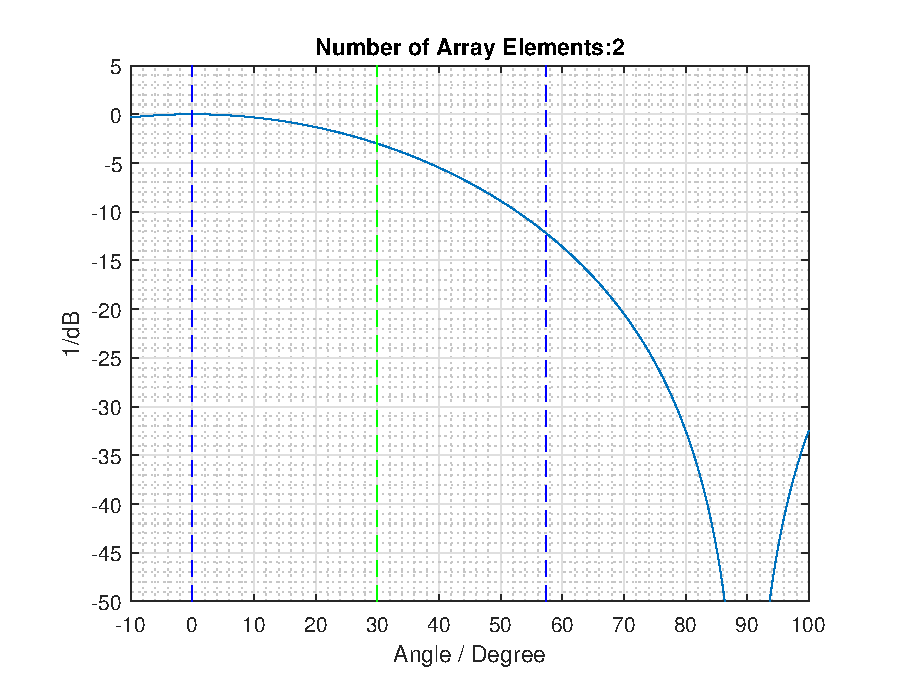
\includegraphics[width=0.32\textwidth]{Matlab/NoNumEl2.eps}}
  \centering
  \subfigure[Six elements: Pattern]{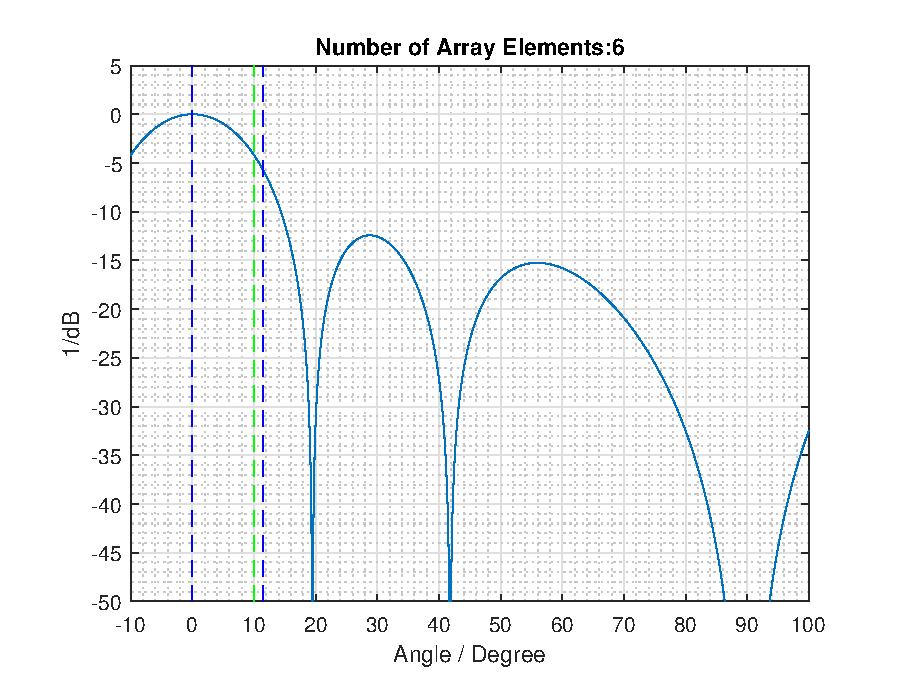
\includegraphics[width=0.32\textwidth]{Matlab/NoNumEl6.eps}}
  \centering
  \subfigure[100 elements: Pattern]{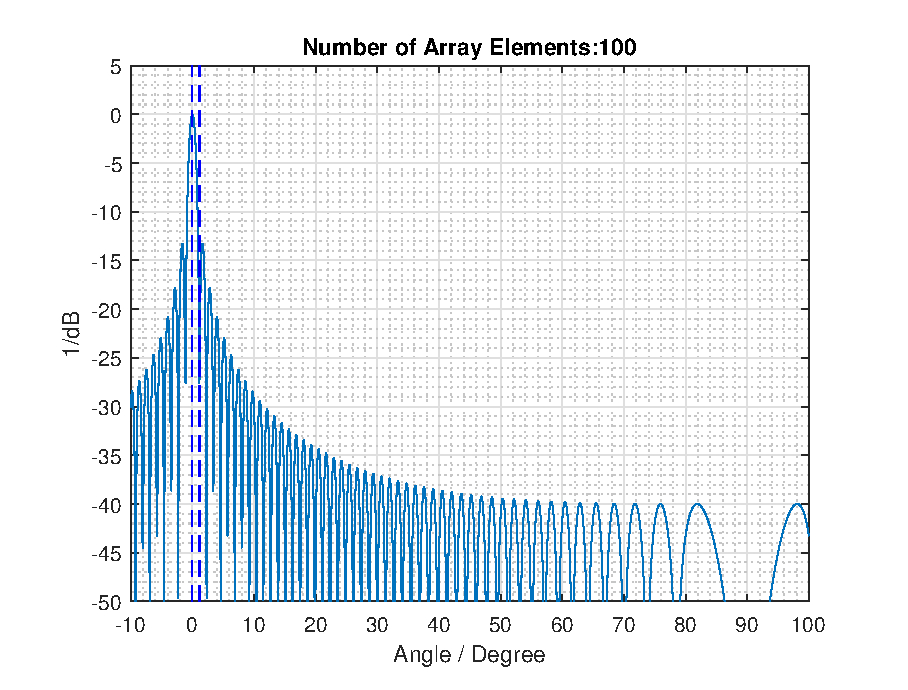
\includegraphics[width=0.32\textwidth]{Matlab/NoNumEl100.eps}}
\caption{Pattern of $N$-element array with $\sfrac{\lambda}{2}$-spacing}
\label{fig:evolvpattern2}
\end{figure}

\begin{figure}[h]
  \centering
  \subfigure[Two elements: Mode spectra]{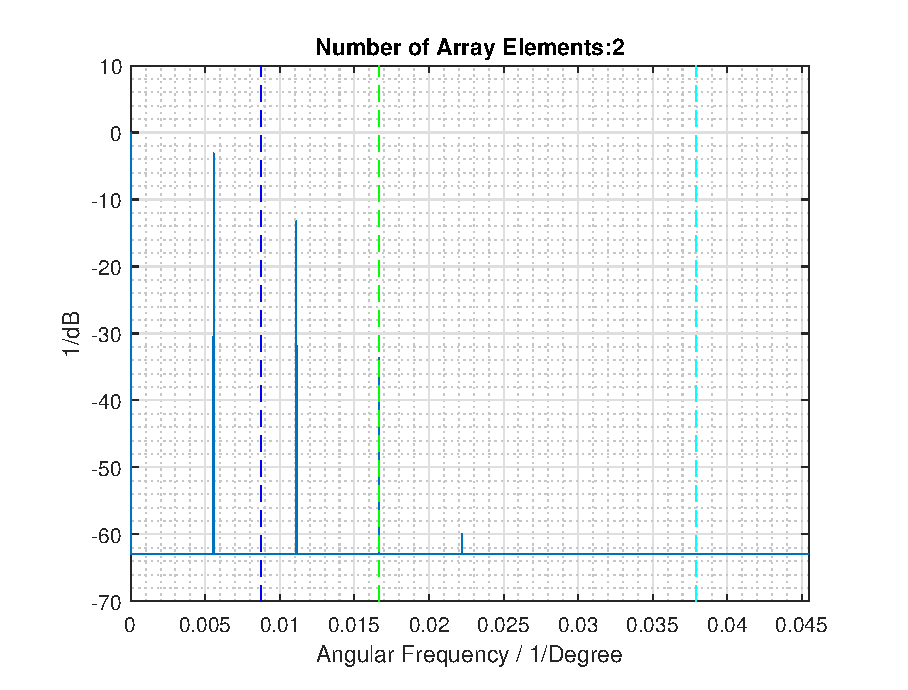
\includegraphics[width=0.32\textwidth]{Matlab/SpNumEl2.eps}}
  \centering
  \subfigure[Six elements: Mode spectra]{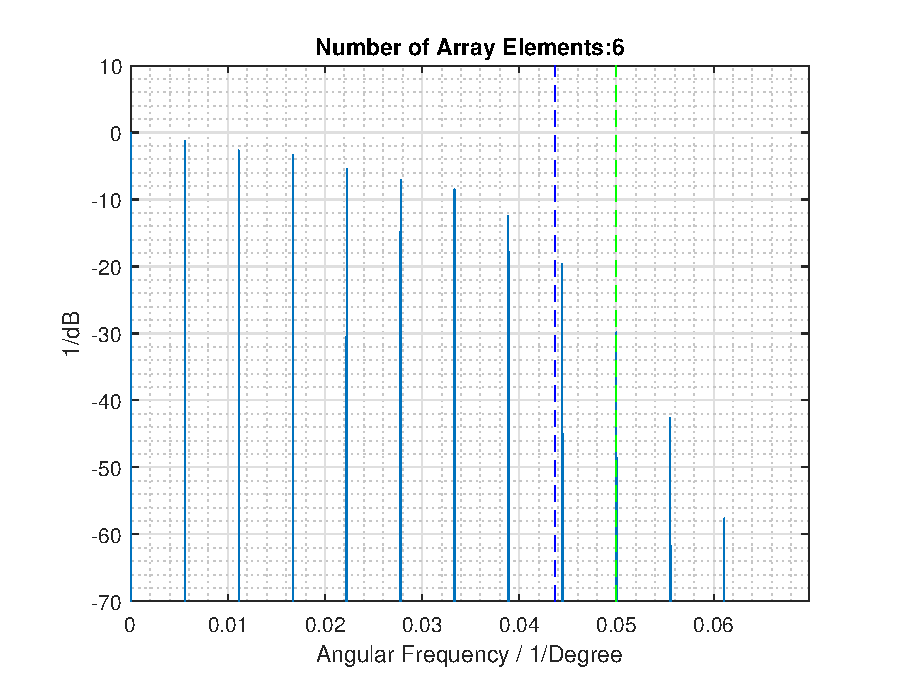
\includegraphics[width=0.32\textwidth]{Matlab/SpNumEl6.eps}}
  \centering
  \subfigure[100 elements: Mode spectra]{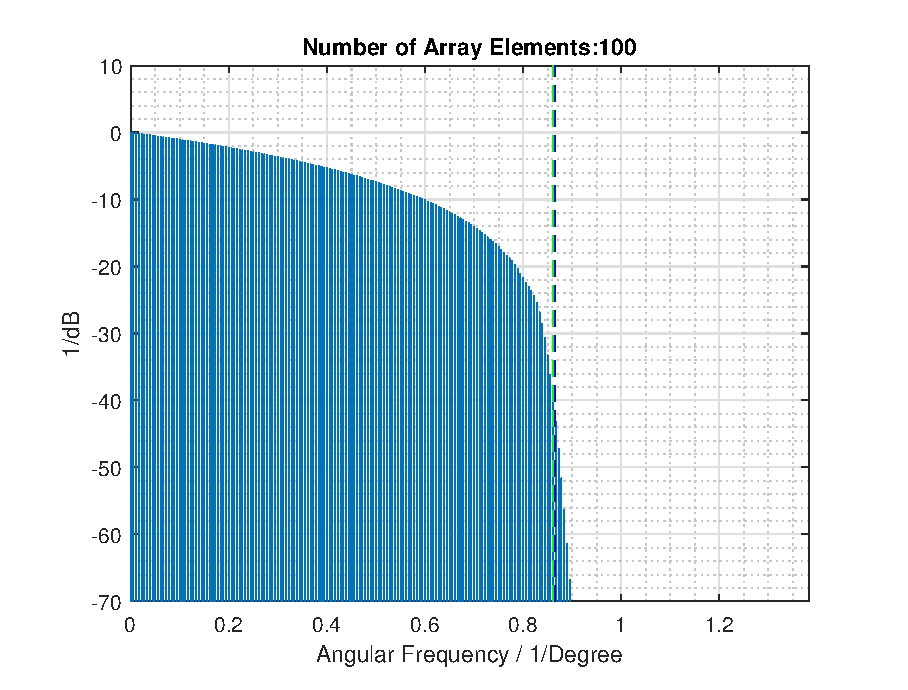
\includegraphics[width=0.32\textwidth]{Matlab/SpNumEl100.eps}}
\caption{Mode spectra of $N$-element array with $\sfrac{\lambda}{2}$-spacing}
\label{fig:evolvpattern3}
\end{figure}

The resulting pattern is depicted in figure \ref{fig:evolvpattern2} and in annex \ref{fig:evolvpattern} (a little larger).\\
In \cite{hansen} it is suggested to use the sampling increment of:

\begin{equation}
\Delta\Theta_\text{Hansen} = \frac{2\pi}{2N+1}\ , \quad \Delta\Phi_\text{Hansen}=\frac{2\pi}{2M+1}
\label{eq:refahansen}
\end{equation}

Where $N$ is the highest significant wave mode on the minimum sphere enclosing the antennas aperture and $M$ is the highest significant wave mode on the minimum cylinder. With the sphere radius $r_S$, the cylinder radius $r_C$ and the angular wavenumber $k = \sfrac{2\pi}{\lambda}$ they are calculated as follows:

\begin{equation}
N = kr_S+10\ , \quad M = kr_C+10
\end{equation}

For example, the resulting formula for the reference angle increment in elevation is calculated in \cite{2018arXiv180310993F} as

\begin{equation}
\Delta\Theta_{\text{ref}} = \lim_{r_S \to \infty}\Delta\Theta' = \lim_{r_S \to \infty} \frac{2\pi}{2\left(kr_S+10\right)+1} = \frac{\lambda}{2\cdot r_S},
\label{eq:hansenrefa}
\end{equation}

the reference angle increment in azimuth as

\begin{equation}
\Delta\Phi_{\text{ref}} = \frac{\lambda}{2\cdot r_C}.
\end{equation}

To illustrate these angle increments the one dimensional array of isotropic radiators is taken. Evaluating the \ac{AF} of a $d = \sfrac{\lambda}{n}$ -array with $N$ elements the reference angle becomes very short:

\begin{equation}
\Delta\Phi_{\text{ref}} = \frac{n}{N-1}
\label{eq:1dinc}
\end{equation}

With the \ac{FFT} over the angle of the antenna patterns from figure \ref{fig:evolvpattern2} the mode spectra can be derived and is seen in figure \ref{fig:evolvpattern3} (or \ref{fig:evolvpattern} in annex).\\
When an arbitrary signal is sampled, the spectrum is mirrored at the sampling frequency. Choosing a sampling frequency lower than twice the highest occurring frequency in the sampled signal causes an irreversible error. This is called the Nyquist-Shannon sampling theorem.\\
For that sake the dashed lines are:

\begin{equation}
\color{blue}\left(\Delta\Phi_{\text{ref}}\right)^{-1}\color{black},\ \color{cyan}\left(\Delta\Phi_\text{Hansen}\right)^{-1}\color{black}\ \text{and}\ \color{green}\text{first mode} > \SI{-40}{\decibel} \color{black}
\end{equation}

Similar to that the dashed lines in figure \ref{fig:evolvpattern2} are the first sampling points using the derived sampling frequency.\\
The issue is now to find the sampling frequency at which the sampling error is independent from the aperture of the antenna. As depicted in figure \ref{fig:evolvpattern3} the sampling frequency introduced by \cite{hansen} is to strict for small apertures. On the other hand the reference angle introduced by \cite{2018arXiv180310993F} is to inaccurate for small apertures. Because of that the new \ac{CrefA} is taken:

\begin{equation}
\text{CrefA} = \left(\Delta\Phi_{\text{ref}}\cdot\left(\text{first mode} > \SI{-40}{\decibel}\right)\right)^{-1}
\end{equation} 

\begin{figure}
\centering
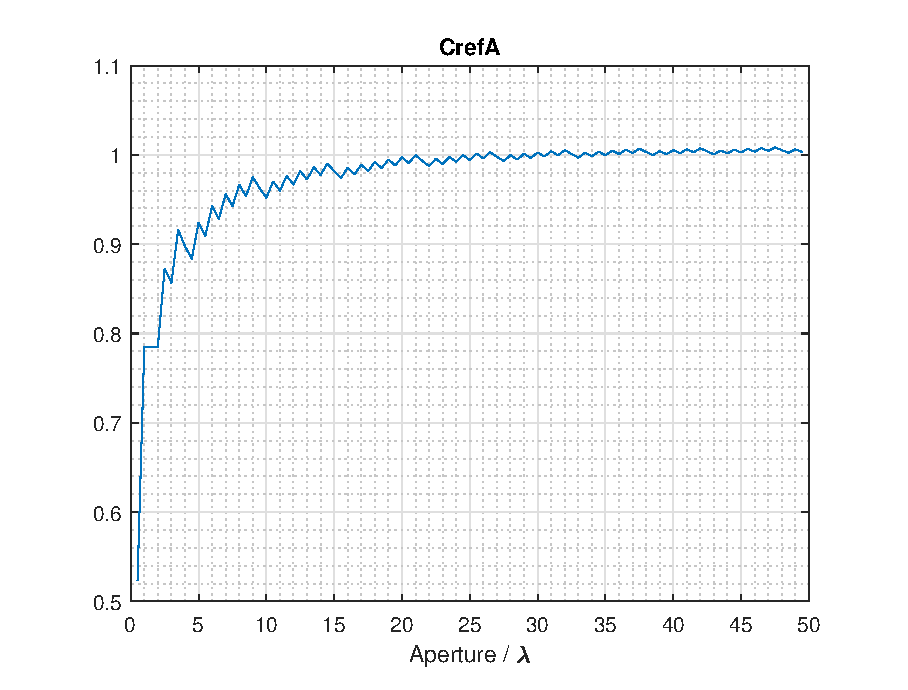
\includegraphics[width=0.41\textwidth]{Matlab/CrefA.eps}
\caption{Correction Factor Reference Angle}
\label{fig:crefa}
\end{figure}

This factor is plotted in figure \ref{fig:crefa}. It is dependent of the aperture. With that the error due to sampling is independent from the antennas aperture. Less than $\SI{-40}{\decibel}$ in the mode spectra is defined for the reference angle increment in \cite{2018arXiv180310993F}, compare figure \ref{fig:evolvpattern3}.\\
For further reduction of points a second factor is introduced, the \acf{SF}. At $\text{SF}=2$ every second measurement point is skipped. With all that the angle increments for spherical sampling is:

\begin{equation}
\Delta\Theta = \text{SF}\cdot\text{CrefA}\left(\sfrac{2r_S}{\lambda}\right)\cdot\frac{\lambda}{2r_S}\ ,\quad\Delta\Phi = \text{SF}\cdot\text{CrefA}\left(\sfrac{2r_C}{\lambda}\right)\cdot\frac{\lambda}{2r_C}
\label{eq:angle}
\end{equation}

\subsection{Constant Step Size Grid}


\begin{figure}[h]
  \centering
  \subfigure[$\text{CTF}=0$; spherical presentation]{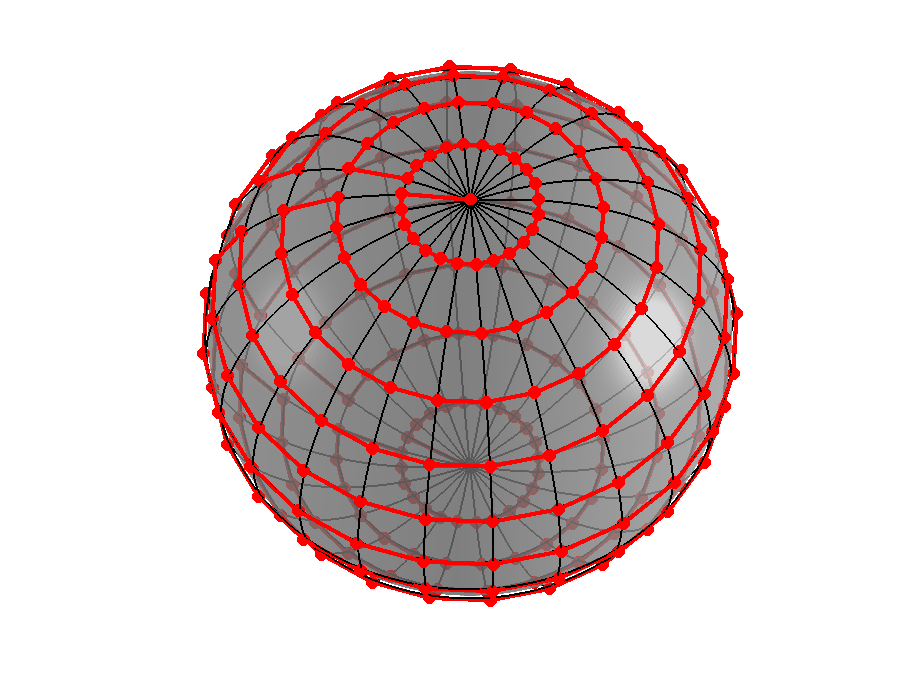
\includegraphics[width=0.49\textwidth]{Matlab/GridCoStPolar.eps}}
  \centering
  \subfigure[$\text{CTF}=1$; spherical presentation]{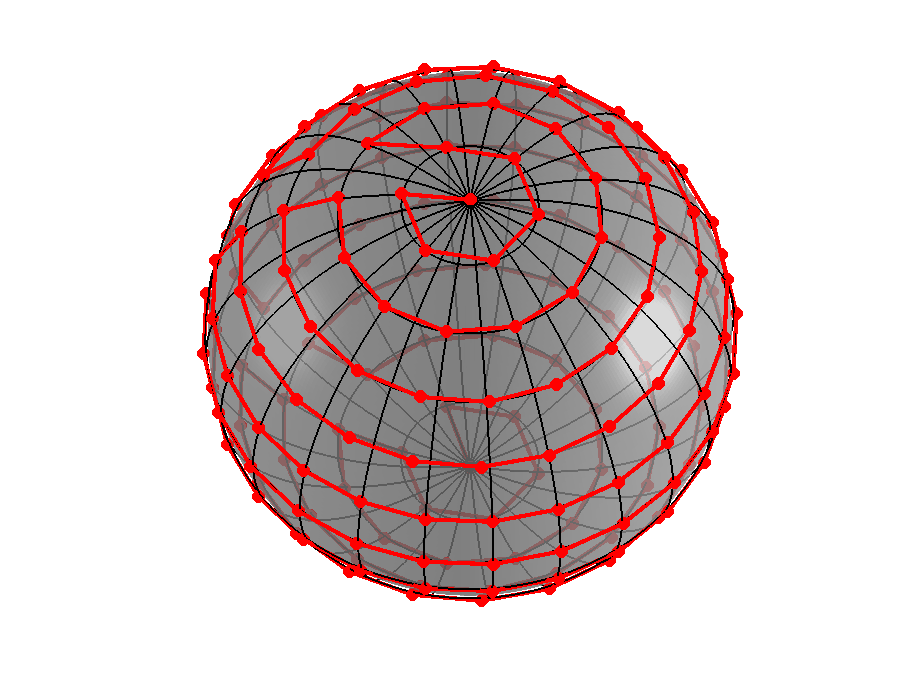
\includegraphics[width=0.49\textwidth]{Matlab/GridCoStSinPolar.eps}}
  \centering
  \subfigure[$\text{CTF}=0$; Cartesian presentation]{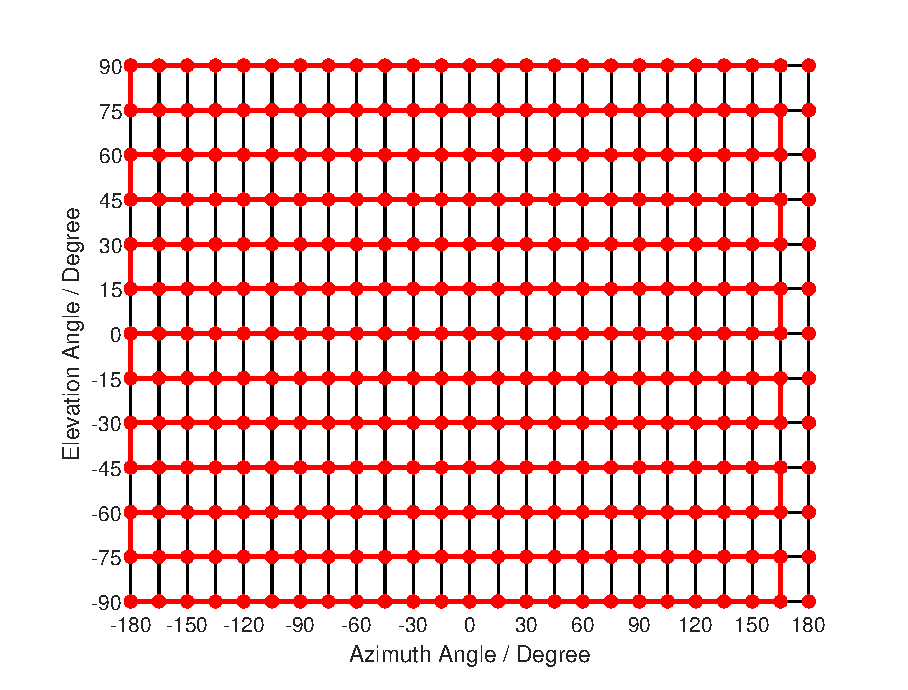
\includegraphics[width=0.49\textwidth]{Matlab/GridCoStCart.eps}}
  \centering
  \subfigure[$\text{CTF}=1$; Cartesian presentation]{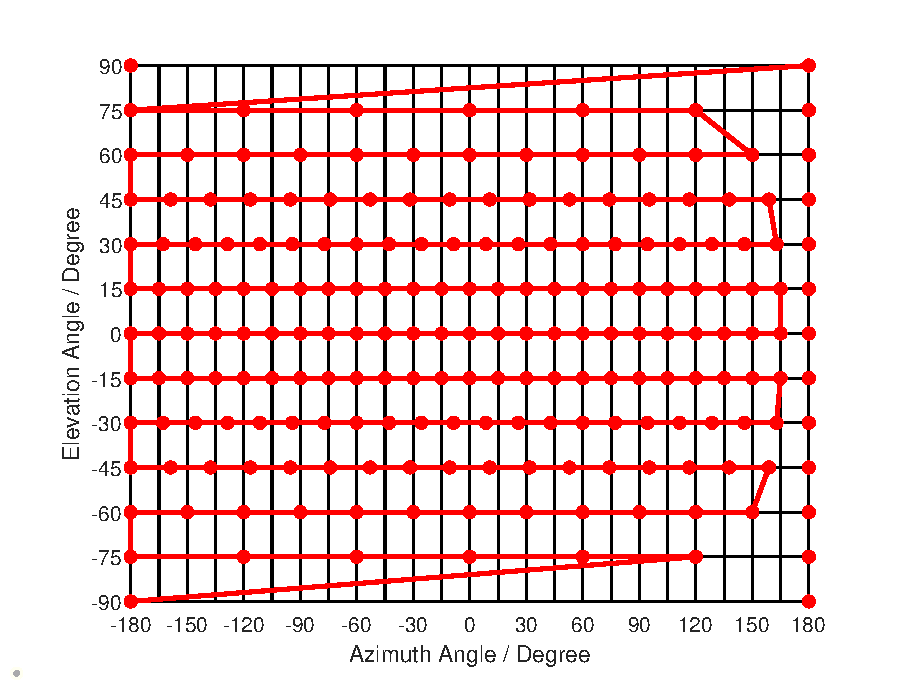
\includegraphics[width=0.49\textwidth]{Matlab/GridCoStSinCart.eps}}
\caption{$\SI{15}{\degree}$ -Constant Step Size Grid}
\label{fig:cssg}
\end{figure}

The most straight forward way to a spherical measurement is using a \ac{CSSG} depicted in figure \ref{fig:cssg} (a). The advantage is the easy feasibility with any positioner. This is visual in \ref{fig:cssg} (c), where the angles are printed in Cartesian coordinates. Ether the azimuth can be swept on every latitude circle or the elevation can be swept on every longitude circle. On the other hand the measurement density is higher on the poles than on the equator.\\
To meet that the theta dependent number of azimuth points was introduced e.g. by \cite{ctiaat}. It is applied as follows:

\begin{align}
N_{\text{max}} = \frac{2\pi}{\Delta\Phi}\\
N\left(\Theta\right)=\lceil N_{\text{max}}\cdot\cos\left(\Theta\right)\rceil\\
\Delta\Phi\left(\Theta\right) = \frac{2\pi}{N\left(\Theta\right)}
\end{align}

It is only possible to sweep the azimuth when this type of grid is used. Here also the Cartesian coordinates are plotted in (d). The red line is a suggested sequence.

\subsection{Constant Density}

\begin{figure}[h]
  \centering
  \subfigure[Polar Coordinates]{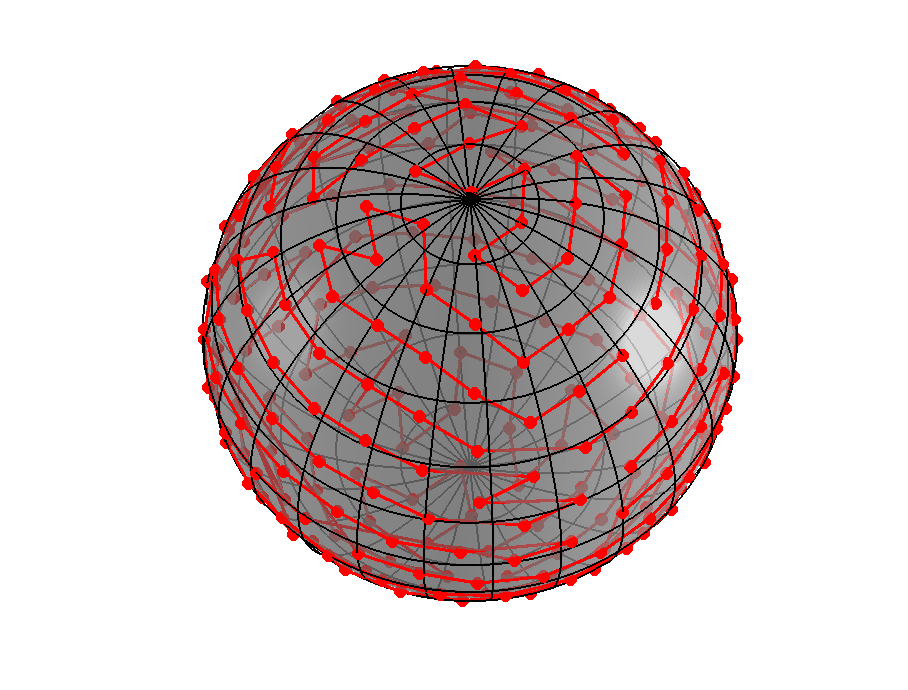
\includegraphics[width=0.49\textwidth]{Matlab/GridCoDePolar.eps}}
  \centering
  \subfigure[Cartesian Coordinates]{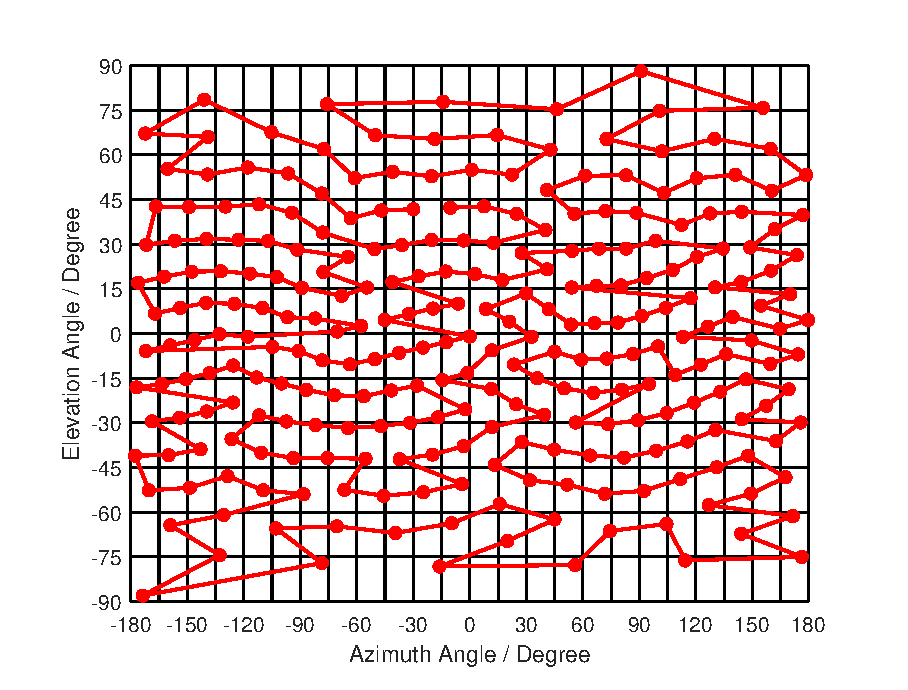
\includegraphics[width=0.49\textwidth]{Matlab/GridCoDeCart.eps}}
\caption{Constant Density Grid with 264 Measurement points}
\label{fig:cdg}
\end{figure}

The \ac{CDG} depicted in figure \ref{fig:cdg} was produces and generated by a charged particle algorithm. It works by minimising the cumulated potential energy of all measurement dots considered as charged particles. The potential energy is minimal, when all points are evenly distributed over the sphere.\\ 
Deriving the optimal measurement sequence is a \ac{TSP}. It is solved by the Matlab toolbox introduced in \cite{tsp} viewing the angles as Cartesian coordinates. This path is optimized for the positioner to move as efficient as possible. Because the positioning in Azimuth is faster than in Elevation, the elevation distance is weighted five times more. Furthermore the periodicity is taken to account, so that the distance between tow points $\text{P}_n$ and $\text{P}_m$ is:

\begin{equation}
\Delta\Theta_{mn} = 5\left(\Theta_{\text{P}_n}-\Theta_{\text{P}_m}\right)\ ,\quad \Delta\Phi_{mn} = \text{min}\left(|\Phi_{\text{P}_n}-\Phi_{\text{P}_m}|\, ,\ 2\pi-|\Phi_{\text{P}_n}-\Phi_{\text{P}_m}|\right)
\end{equation}

With that the quadratic distance Matrix $D$ can be derived using euclidean distance with $d_{mn} = \sqrt{\Delta\Theta_{mn}^2+\Delta\Phi_{mn}^2}$ out of $N$ Points:

\begin{equation}
D = \begin{bmatrix}
 0 & d_{12} & \dots & d_{1N}\\
 d_{21} & 0 & \dots & d_{2N}\\
 \vdots & \vdots & \ddots & \vdots\\
 d_{N1} & d_{N2} & \dots & 0
\end{bmatrix}
\end{equation}

The cumulated distance for $N = 264$ is converged after around one million iterations. The result is depicted in figure \ref{fig:cdg} (b).

\subsection{Other}

There are other grid types, which are mainly based on the already introduced grids. First there are Cardinal cuts, here a measurement is carried out along the equator and one, tow or more orthogonal meridians. If the alignment is right a technique called \acf{PM} can be used to calculate the complete antenna pattern out of the cardinal cuts. The problem here is that a symmetry is assumed which is always wrong if the direction of main beam and the orientation of the pattern is unknown. \cite{2018arXiv180310993F}\\
An other spatial sampling approach is the Spiral Scan. It is developed by \ac{RS} and can be used for a pre scan to find the maximum \ac{EIRP} direction. Here elevation and azimuth is swept. \cite{ctiaat}

\section{Total Radiated Power Quadratures}
\label{sec:quadrature}

The easiest way to derive the \ac{TRP} is if Cardinal cuts or a \ac{CDG} was taken, to compute the mean of all \ac{EIRP} samples. For other grids the quadrature needs to be done as follows. \cite{trp}

\subsection{Sine Theta}

The straight forward way is to transform the integral over a spherical surface $S$

\begin{equation}
\text{TRP} = \frac{1}{4\pi}  \oiint_S \text{EIRP}\left(\theta,\phi\right)\cdot\sin\theta\cdot d\theta d\phi
\label{eq:trpint}
\end{equation}

to a sum, this is called quadrature. The easiest approach is carried out by discretizing the integral Argument:  \cite{ctiaat}

\begin{equation}
\frac{1}{4\pi}\cdot\sin\theta\cdot d\theta\cdot d\phi \ \Rightarrow\ \frac{1}{4\pi}\cdot \Delta\theta\cdot \Delta\phi\cdot\sin\theta = \frac{1}{4\pi}\cdot \frac{\pi}{N}\cdot \frac{2\pi}{M}\cdot\sin\theta=\frac{\pi}{2NM}\cdot\sin\theta
\end{equation}

With that the quadrature is:

\begin{equation}
\text{TRP}_{\sin\theta} = \frac{\pi}{2NM}\sum^{N-1}_{i=1}\sum^{M-1}_{j=0}\left(\text{EIRP}_\theta\left(\theta_i,\phi_j\right)+\text{EIRP}_\phi\left(\theta_i,\phi_j\right)\right)\cdot\sin\left(\theta_i\right)
\label{eq:trpsumsin}
\end{equation}

$N$ is the number of angular intervals in $\theta=\left[0,\pi\right[$ (elevation), $M$ is the number of angular intervals in $\phi=\left[0,2\pi\right[$ (azimuth), the indices $i=\left[0,N\right]$, $j=\left[0,M\right]$ and the \ac{EIRP} is split in its horizontal ($\text{EIRP}_\phi$) and its vertical ($\text{EIRP}_\theta$) part. This quadrature is called sine theta.

\subsection{Clenshaw-Curtis}

Because the sine theta quadrature is not accurate for spars measurements and the measurement points at the poles are neglected, an other weighting scheme is used, the \ac{CC}-quadrature. For the sine theta quadrature the integrating surface is constantly interpolated (compare equation \ref{eq:trpsumsin}). The \ac{CC} quadrature is more accurate using the weights W computed by expending the integrand with Chebyshev polynomials. With that formula \ref{eq:trpsumsin} develops to: \cite{trp}

\begin{equation}
\text{TRP}_{\text{CC}} = \frac{1}{2M}\sum^{N-1}_{i=1}\sum^{M-1}_{j=0}\left(\text{EIRP}_\theta\left(\theta_i,\phi_j\right)+\text{EIRP}_\phi\left(\theta_i,\phi_j\right)\right)\cdot\text{W}\left(\theta_i\right)
\label{eq:trpsumcc}
\end{equation}

\subsection{Jacobi}

The Jacobi quadrature uses the area of triangles on the spherical surface between the measurement points. The average \ac{EIRP} of a triangle is computed and weighted by the area $A_i$ of it. The result is normed with the complete surface area. With that for every triangle $i=\left[1,N\right]$ the \ac{TRP} quadrature is: \cite{trp}

\begin{equation}
\text{TRP}_{\text{J}} = \frac{\sum^N_{i=1}A_i\left(\frac{\text{EIRP}_{0,i}+\text{EIRP}_{1,i}+\text{EIRP}_{2,i}}{3}\right)}{\sum^N_{i=1}A_i}
\end{equation}

\subsection{Comparing the Quadratures}

Sine Theta- and \ac{CC} quadratures are only applicable for \acp{CDG} and with slight optimizations also for \acp{CDG} with less dense measurements at the poles. Whereas the Jacobi quadrature can be used for arbitrary grids.\\
In \cite{trp2} it is investigated which quadrature leads to the most accurate result with the same number of points. The result is that \ac{CC}- and Jacobi quadratures are equally accurate.

\section{Statistics and Regression}

This section shall give a brief introduction in the field of statistics and regression, which is necessary for the spatial sampling simulation. First statistical terms, than methods to display scatterings and multidimensional regressions are introduced.

\subsection{Metrics to Describe Distributions}

To describe a one dimensional scattering $h$ with $N$ samples $x$ and the cumulative frequency $H$, these terms are regularly used: \cite{dffs}

\begin{itemize}
\item The commonly most used and known term is the \textbf{Arithmetic Mean}, which is vulnerable by outliers and computed as:
\begin{equation}
\bar x = \frac{1}{N}\sum_{n=1}^N x_N
\end{equation}
\item The \textbf{Median} is that value lying in the middle of a distribution, so that $H\left( x\right) = 0.5$. It is computed by sorting the samples by value and, if the number of samples is even, taking the mean of the two samples in the middle, or if the number of samples is odd taking the middle value.
\item The \textbf{Variance} of a distribution is the sum of squared error, normalized by the number of samples. This metric is strongly vulnerable by outliers. The computation is as follows:
\begin{equation}
s^2 = \frac{1}{N-1}\sum_{n=1}^N\left( x_n-\bar{x}\right)^2
\end{equation}
\item The \textbf{$p$-Quantile} is analogue to the Median, that value of a sorted sample vector where $P$ percent of the distributions values is reached, hence $H\left( x\right) = p$.
\item A more stable metric for scattering as the variance is the \textbf{\ac{IQR}}, this describes the range between two quantiles.
\end{itemize}

\subsection{Display a Distribution}

The commonly known way to display a distribution is a bar diagram. There the value of range is split in $M$ bars displaying the values in the $x$-axis and the probability of each bucket on the $y$-axis. An other way to display a distribution is the box-plot, where only the minimal, maximal, $\SI{25}{\percent}$-quantile, median and $\SI{75}{\percent}$-quantile value is plotted.

\subsection{Distribution Functions}
There are all sorts of scattering distributions e.q. even distribution, Weibull distribution, Rayleigh distribution, ... but the most prominent distribution is the normal distribution by Gauss:

\begin{equation}
f\left( x \right) = \frac{1}{\sigma\sqrt{2\pi}}e^{-\frac{1}{2}\left(\frac{x-\mu}{\sigma}\right)^2}
\end{equation}

Assuming that $\sigma = s$ and $\mu = \bar{x}$ this function can also be plotted and used for predictions.

\subsection{Regression of multidimensional Datasets}
\label{sec:regod} 
Assuming a input variable vector $\vec{x}$, a coefficient set $\vec{b}$ and a result $y$ an arbitrary polynomial can be written as: \cite{sip}

\begin{equation}
y\left(\vec{x}\right) = \vec{x}^{\mathsf T}\cdot\vec{b}=\begin{bmatrix}
1 & x_1 & x_2 & \dots & x_M
\end{bmatrix} \cdot \begin{bmatrix}
b_0 \\ b_1 \\ b_2 \\ \vdots \\ b_M
\end{bmatrix}
\end{equation}

The regression is about estimating the coefficient vector $\vec{b}$. With $N$ samples this system is overdetermined which leads to an error vector $\vec{e}$. Than the resulting polynomial is:

\begin{equation}
\vec{y}=X\cdot \vec{b}+\vec{e}=\begin{bmatrix}
y_1 \\ y_2 \\ \vdots \\ y_N
\end{bmatrix} = \begin{bmatrix}
1 & x_{11} & x_{12} & \dots & x_{1M} \\
1 & x_{21} & x_{22} & \dots & x_{2M} \\
\vdots & \vdots & \vdots & \ddots & \vdots \\
1 & x_{N1} & x_{N2} & \dots & x_{NM}
\end{bmatrix} \cdot \begin{bmatrix}
b_0 \\ b_1 \\ b_2 \\ \vdots \\ b_M
\end{bmatrix} + \begin{bmatrix}
e_1 \\ e_2 \\ \vdots \\ e_N
\end{bmatrix}
\end{equation}

The sum square error

\begin{equation}
S = \vec{e}^{\mathsf T}\cdot\vec{e}=\left(\vec{y}-X\cdot\vec{b}\right)^{\mathsf T}\cdot\left(\vec{y}-X\cdot\vec{b}\right)
\end{equation}

is minimized by 

\begin{equation}
\nabla_{\vec{b}}\cdot S = 0
\end{equation}

leading to the well known \ac{LS}-method

\begin{equation}
\hat{b}_\text{LS}=\left(X^{\mathsf T} X\right)^{-1} X^{\mathsf T}\vec{y}.
\end{equation}

The input matrix $X$ can also be optimized by taking combinations or powers of different dependent parameters.\\
A frequent problem is that the significance of the parameters in $\vec{b}$ is unknown, hence to unnecessary high number of parameters and inaccurate regressions. Therefore the hypothesis that $b_m=0$ is checked. The parameters in vector $\vec{b}$ are t-distributed. First the covariance matrix of the independent variable $\vec{y}$ is estimated: \cite{dffs}

\begin{equation}
C = \left(X^{\mathsf T} X\right)^{-1}\frac{1}{N-M-1}\cdot\left(\vec{y}^{\mathsf T}\cdot\vec{y}-\vec{b}^{\mathsf T}\cdot X^{\mathsf T}\cdot \vec{y}\right) = \begin{bmatrix}
c_{00} & c_{01} & \dots & c_{0M} \\
c_{10} & c_{11} & \dots & c_{1M} \\
\vdots & \vdots & \ddots & \vdots \\
c_{M0} & c_{M1} & \dots & c_{MM}  
\end{bmatrix}
\end{equation}

With the variances $c_{mm}$ of each parameter and the variance of $\vec{y}$ $s$, the $p$-value can be computed with $F_t$, the \ac{CDF} of the t-distribution with $N-1$ degrees of freedom:

\begin{equation}
p_m = F_t\left(\frac{b_m}{c_{mm}\cdot s}\right)
\end{equation}

Normally a significance value of $\alpha = \SI{5}{\percent}$ is chosen. If the $p$-value is inside the interval $p_m=\left[\sfrac{\alpha}{2},\ 1-\sfrac{\alpha}{2}\right]$ the hypothesis is valid and parameter $m$ can be discarded.

To estimate the confidence interval for the mean of a regression at a point $x_0$ the variance at dot $x_0$ must be computed: \cite{dffs}

\begin{equation}
s_{\hat{y}_0}^2 = \frac{1}{N-M-1}\cdot\left(\vec{y}^{\mathsf T}\cdot\vec{y}-\vec{b}^{\mathsf T}\cdot X^{\mathsf T}\cdot \vec{y}\right)\cdot \vec{x}_0^{\mathsf T}\cdot \left(X^{\mathsf T} X\right)^{-1} \cdot \vec{x}_0
\end{equation}

Choosing a confidence value $\gamma = \SI{95}{\percent}$, the two parameters $k_1$ and $k_2$ can be derived with the inverse \ac{CDF} $F_t^{-1}$ with $N-M-1$ degrees of freedom:

\begin{equation}
k_1 = F^{-1}\left(\frac{1-\gamma}{2}\right),\ k_2 = F^{-1}\left(\frac{1+\gamma}{2}\right)
\end{equation}

And the confidence interval is:

\begin{equation}
\mu_y\left(\vec{x}_0\right) =\left[ y\left(\vec{x}_0\right)-k_2\cdot s_{\hat{y}_0},\ y\left(\vec{x}_0\right)-k_1\cdot s_{\hat{y}_0}\right]
\label{eq:conv}
\end{equation}



\chapter{Regulatory Test System}  \label{chap:3}

The standard Regulatory Test System (TS8997) by \acs{RS}\textregistered{} verifies technologies typically used in wideband wireless devices, i.e. devices with a radio interface, in the 2.4 GHz and 5 GHz band: \acs{WLAN} \acs{IEEE} 802.11a/b/g/n/ac, Bluetooth\textregistered, wireless video transmission and radio remote control. The test system consists of a Signal Generator, Spectrum Analyzer,  \acf{CMW}, and a Switching Unit (OSP-B157W8). My thesis investigates the approach of normalized measurements using the \acs{RF} Shielded Box and a Switching Unit (OSP-B157WN), which is an extension to the current standard regulatory test system. This extension is required for the normalized measurements.

\begin{figure}[H]
\centering
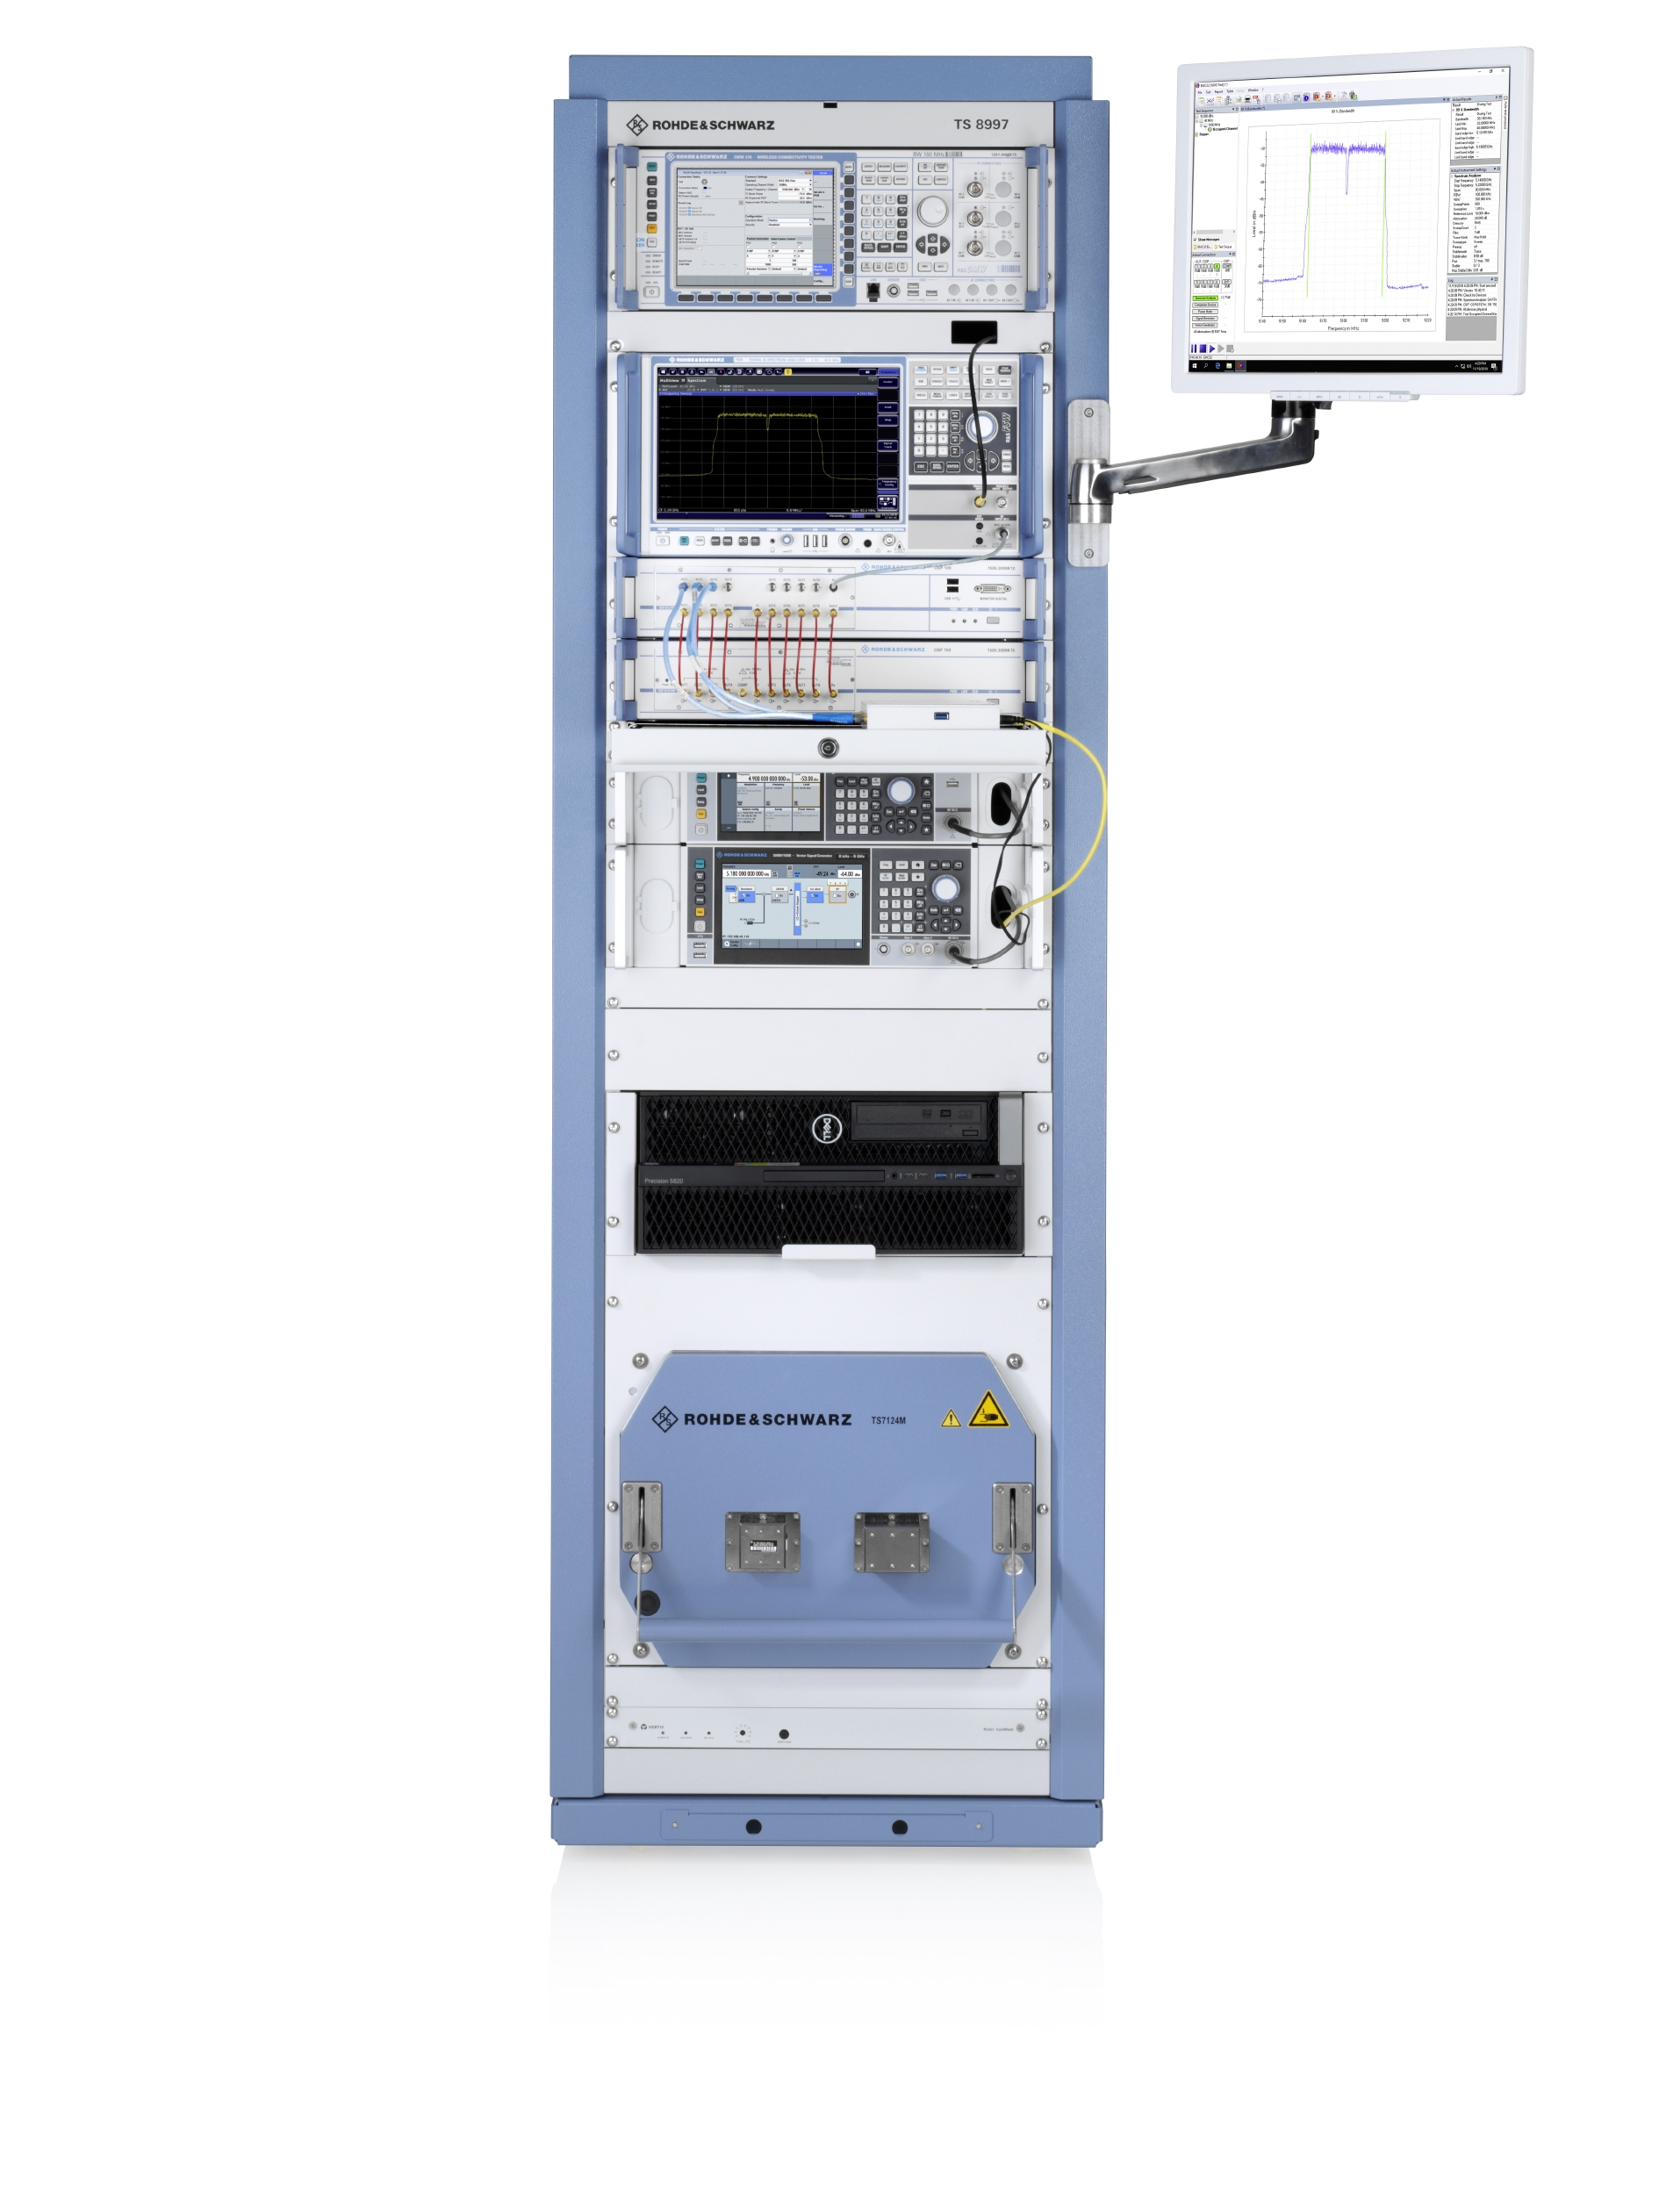
\includegraphics[width=0.5\textwidth]{TestSystem.jpg}
\caption{\acs{RS}\textregistered{} Test System - TS8997}
\label{fig:testsystem}
\end{figure}

This chapter includes all the instruments / equipments required for this thesis. Each section describes in brief about the instrument / software.

\section{WMS32 Software Suite}
\label{sec:wms32}
WMS32 software suite comes with the standard regulatory test system (TS8997). The software features loading, starting, and stopping, pausing, and saving of tests. This software is used only for conducted measurements. In this thesis, this software is not made use of because the software is optimized for end users and one cannot have full control over the settings of the instrument which is very much required for academic research. It is not possible to debug and check results at different stages during the tests if the WMS32 software is used. The only way it would be possible is by learning the source code of the software and trying to debug it via the source code. But, since it is not very convenient to do that, I wrote my code from scratch for all the measurement tests. The figure below shows the \acs{GUI} of the WMS32 software.

\begin{figure}[H]
\centering
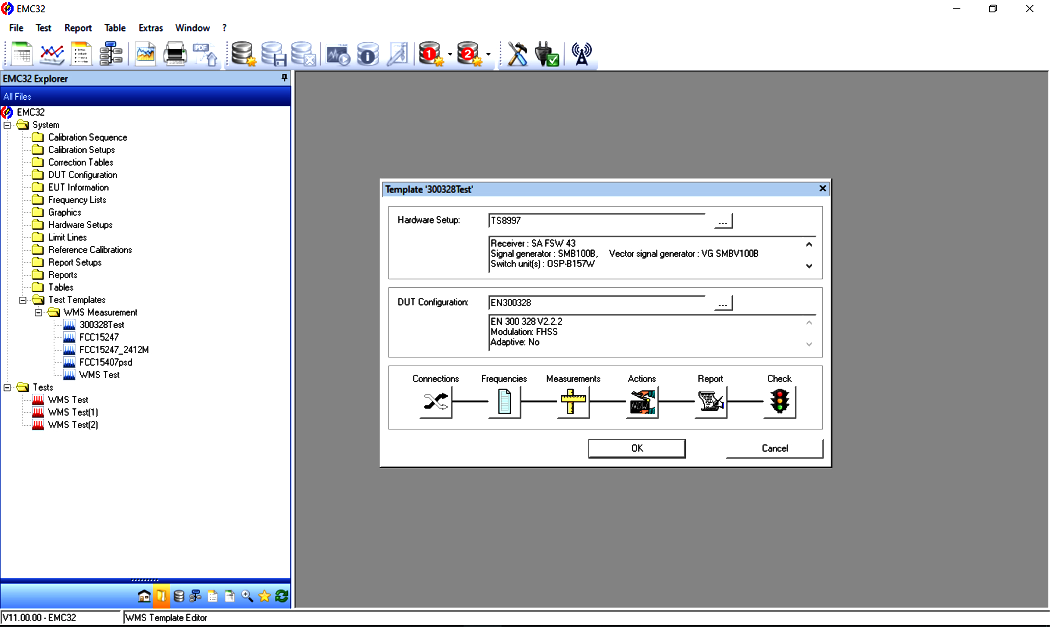
\includegraphics[width=0.8\textwidth]{wms32.pdf}
\caption{\acs{RS} software suite - WMS32}
\label{fig:softwaresuite}
\end{figure}

\section{Spectrum Analyzer}
The analyzer measures the signal either in the frequency domain or in the time domain (zero span). A MATLAB\textregistered{} script is written to remotely access the instrument. The MATLAB\textregistered{} code then calculates the power and bandwidth. The \acf{SCPI} commands for each task (i.e. changing the frequency, span, etc.) are provided in the manual. Few important functions used in this thesis are explained below.

\subsection{Trace Mode}
Signals that are varying are dealt with by setting the trace mode in the spectrum analyzer. The available modes are Clear/Write, \acs{Max-Hold}, or Average.
\begin{enumerate}
  \item Clear/Write is used when new overwritten values are needed on every sweep. It shows what is coming in, as it happens. The change in the signal during the sweep causes the trace level to change. 
  \item \acs{Max-Hold} stores the sweep only when the new value is greater than the previous one. The maximum value of the signal can be thus determined over several sweeps. This makes the trace continue to increase as various signals come and go. If a signal shows up once, it is saved on the Max-Hold trace. Setting trace 1 to normal, and trace 2 to \acs{Max-Hold} is useful in many situations, as it shows both the current power level and the excursion limits.  
  \item Average Mode activates the averaging function of the trace. The average is formed over several sweeps. The number of sweeps is selected by the user. The average model is good, but a slow, tool to remove random noise and highlight constant signals. It is great when the signal you are interested in is near the noise floor of the instrument.  
  \end{enumerate}

\subsection{Detector Settings}
Spectrum analyzers normally sample many more data points than they can display on the screen - tens, hundreds, or thousands of times more. This implies that the displayed trace needs to be summarized in some manner to choose the value to be displayed on each pixel of the screen. This is done by the detectors. The six main detectors settings are:
\begin{enumerate}
  \item Max Peak / Min Peak: They determine the largest of all positive (max peak) or the smallest of all negative (min peak) peak values of the levels measured at the individual frequencies which are displayed on one sample point (or within a pixel). Even if wide spans are displayed with very narrow resolution bandwidth (span/\acs{RBW} >> number of pixels on the frequency axis), no input signals are lost. Therefore this type of detector is particularly useful for \acs{EMC} measurements. This detection method is a good complement to a acs{Max-Hold} trace.
  \item Auto Peak: This detector combines the peak detectors. The maximum peak detector and the minimum peak detector simultaneously determine the maximum and the minimum level within a displayed test point and display it as a single measured value. 
  \item Sample: The detector routes through the sampled data without any further evaluation and either displays them directly or, for reasons of speed in case of short sweep times, first writes them into memory and processes them subsequently. If the span to be displayed is much greater than the resolution bandwidth (span/\acs{RBW} >> number of pixels on the frequency axis), input signals are no longer reliably detected. The same unreliability applies when too large tuning steps of the local oscillator are chosen. In this case, signals may not be displayed at the correct level or may be completely lost. This is required by some standards but is not so useful for spectrum monitoring. 
  \item \ac{RMS}: This detector forms the acs{RMS} value of the measured values within a pixel. To do so, the instrument uses the linear voltage after envelope detection. The sampled linear values are squared, summed and the sum is divided by the number of samples (= \acs{RMS}). For logarithmic display, the logarithm is formed from the square sum. For linear display, the root mean square value is displayed. Each sweep point thus corresponds to the power of the measured values summed up in the sweep point. 
  \item Average: The average detector calculates the linear average of all samples contained in a sweep point. To this effect, the instrument uses the linear voltage after envelope detection. The sampled linear values are summed up and the sum is divided by the number of samples (= linear average value). For logarithmic display, the logarithm is formed from the average value. For linear display, the average value is displayed. Each sweep point thus corresponds to the average of the measured values summed up in the sweep point. The average detector supplies the average value of the signal irrespective of the waveform (\acs{CW} carrier, modulated carrier, white noise, or impulsive signal). 
  \end{enumerate}
  
\begin{figure}[H]
\centering
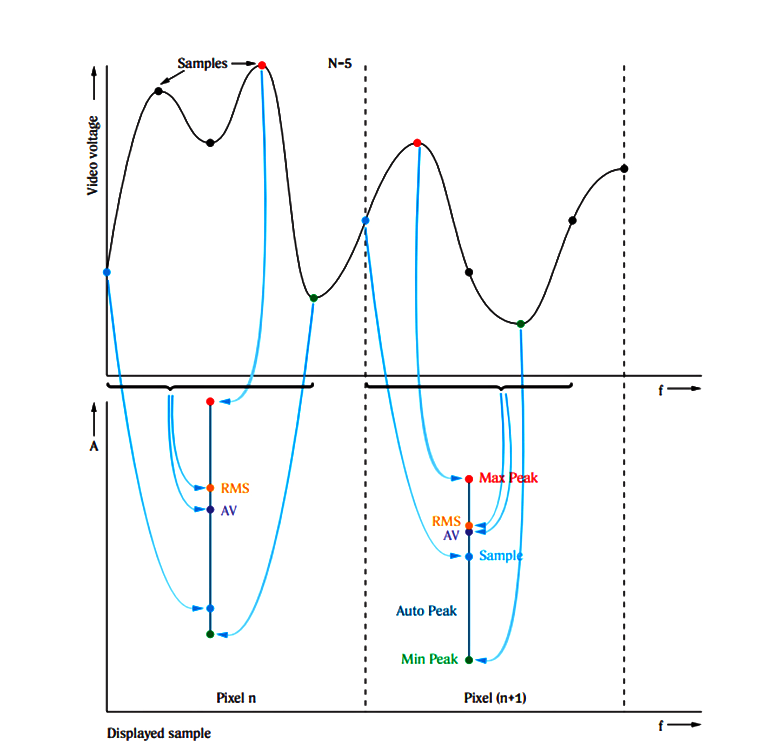
\includegraphics[width=0.7\textwidth]{detectorSetting.pdf}
\caption{Selection of sample to be displayed as a function of detector used}
\label{fig:detectorSettings}
\end{figure}

The choice of detector setting depends on the expected signal. If the signal has a stochastic signal (noise), then the \acs{RMS}-detector is always the best option. This is because the \acs{RMS} detector allows measurement of the actual power of an input signal irrespective of its temporal characteristic. If the crest factor is unknown, the power of random signals (whose instantaneous values are not in line with the Gaussian distribution) can only be determined using an \acs{RMS} detector. When using a sample or max peak detector, the relationship between \acs{RMS} value and peak value must be precisely known for determining the power of signals with random instantaneous value. This knowledge is not required when using an \acs{RMS} detector. The \acs{RMS} value displayed by a specific pixel is calculated from all samples pertaining to this pixel. By increasing the sweep time, the number of samples available for the calculation is increased, thus allowing smoothing of the displayed trace. Smoothing by reducing the video bandwidth or by averaging over several traces is neither permissible nor necessary with the \acs{RMS} detector. The measurement results would be falsified since the displayed values would be too low (max. 2.51 dB). To avoid any falsification of results, the video bandwidth should be at least three times the resolution bandwidth when using the \acs{RMS} detector. If the signal is harmonic, the Max Peak-detector is the correct choice. 


\section{Signal Generator}
\acs{RS}\textregistered{} SMB100A acts as a blocker instrument in this research topic. It is, like other instruments also remotely accessed using \acs{SCPI} commands via a MATLAB\textregistered{} script. It operates in the frequency range of 100 kHz to 40 GHz. The maximum output power is +27 dBm which is sufficient for this thesis. There are better models of signal generators having higher power levels and thus would relax all the limitations caused due to the attenuations in the switching matrix, cables, and isolation between probe antennas. This thesis uses a basic model because it proved to be sufficient for the measurements and also this model is present in almost all test systems. The instrument is used only for the receiver blocking measurement and is used in \acs{CW} signal mode. This means the \acs{RF} signal is generated with the frequency and level set by the user.

\begin{figure}[H]
\centering
\includegraphics[width=0.55\textwidth]{Generator.pdf}
\caption{Signal Generator \acs{GUI}}
\label{fig:gen}
\end{figure}

\section{Companion Device}
In this thesis, a wireless connectivity tester is mainly used as a companion device to communicate with the \acs{DUT} for most of the functions (i.e. power measurement, receiver blocking measurement, occupied channel bandwidth measurement). The wireless connectivity tester can force the \acs{DUT} to be either in transmitter mode or receiver mode. For the \acs{DUT} to be in transmitter mode, the tester sends \acf{ICMP} (ping) packets to the \acs{DUT} and waits for the echo replies from the \acs{DUT}. Because of the low duty cycle (\acs{ICMP} consists of only header data) of the signal from the \acs{DUT}, the results for the power spectral density measurement have a high \ac{MU} explained in later chapter with images). Therefore, a golden device (fritz box) is used as a companion device for this measurement. All the measurements can also be done using this second device but in this thesis, only \ac{PSD} measurement uses the fritz box.

\subsection{Wireless Connectivity Tester} \label{sec:cmw}
\acs{RS}\textregistered{} CMW 270 acts as a base station for mobile communication, Wi-Fi\texttrademark{} \acs{AP}, Wi-Fi\texttrademark{} client, Bluetooth\textregistered{} devices, etc. In this thesis, this device is used as a Wi-Fi\texttrademark{} \acs{AP} because it allows us to perform the required measurements (i.e. \acf{PER}). \acs{WLAN} Signaling mode allows us to associate the \acs{DUT} to the companion device for subsequent tests

\begin{figure}[H]
\centering
\includegraphics[width=0.55\textwidth]{CMW_GUI.pdf}
\caption{Wireless Connectivity Tester \acs{GUI}}
\label{fig:cmwGUI}
\end{figure}

Configuration of \acs{WLAN} signaling is done by sending commands remotely via a MATLAB\textregistered{} script.  The signaling application is configured as \acf{AP}, companion device simulates a \acs{WLAN} \acf{AP} in infrastructure mode. The \acs{DUT} is a \acs{WLAN} station. To establish a \acs{WLAN} association, \acs{WLAN} standard (i.e. \acs{IEEE} 802.11a,g,n), scenario selection (i.e. \acs{SISO} or \acs{MIMO}), Operation Mode (i.e. \acs{AP}), used \acs{RF} connectors, \acs{RF} frequency/channel, power of a transmitted signal (\acs{RF} TX Burst Power) and Expected power of the \acs{DUT} Signal (\acs{RF} Exp. Peak Envelope Power) are set. \acs{RF} TX Burst Power must be sufficient so that the \acs{DUT} can receive the transmitted signal. The \acs{RF} Exp. Peak Envelope Power must be in accordance with the received signal power. The external attenuation is calculated depending on the attenuation from the cable and other devices and is set to the resulted value. To automatize this process, a loop in the MATLAB\textregistered{} script keeps increasing the value of \acs{RF} Exp. Peak Envelope Power until the device connection status says authenticated.

\subsection{Golden Device} \label{sec:golden}

Fritz Box 7590 can be used as a companion device to receive data from the \acs{DUT}. The \acf{NAS} functionality is used to upload data from \acs{DUT} permanently to a pen drive which is attached to the Fritz Box. First, storage is set up on the computer as a network drive. The procedure to mount the network drive is explained on the website of Fritz Box. A windows batch file is written to continuously upload a big file from the DUT to the network drive. The code in the batch (.BAT) file is shown below.

\begin{lstlisting}[language=bash]
:start
copy "C:\source" "Z:\General-UDisk-01" /Y
goto start
\end{lstlisting}

The script copies a big file in a loop and it makes sure to overwrite the existing destination file and hence deleting of the file is not necessary. Since the file is large, the duty cycle of the signal is high and it results in \ac{PSD} measurement having lower measurement uncertainty. 

\begin{figure}[H]
\centering
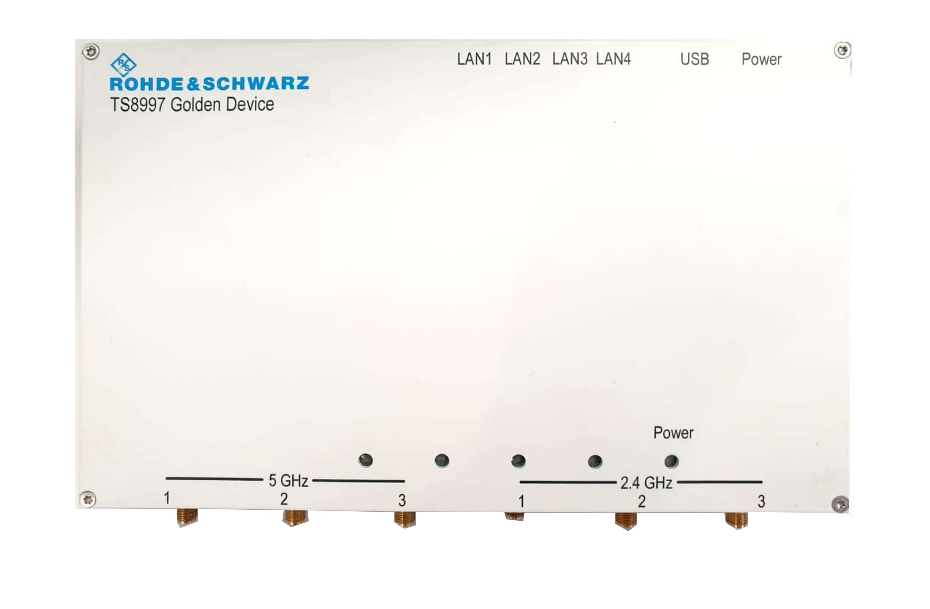
\includegraphics[width=0.55\textwidth]{fritz.pdf}
\caption{\acs{RS}\textregistered{} Golden device (\acs{CMW})}
\label{fig:cmwGUI}
\end{figure}

\section{Switching Units}
These Open Switch and Control Platform can be used to perform \acs{RF} switch and control tasks. This thesis uses two of these switching units. It is convenient to have a dedicated device instead of changing the setup for every test case like in the case of splitters and attenuators. The description and usage are explained below.

\subsection{\acs{RS}\textregistered{} \ac{OSP}-B157WN} \label{sec:wn}
This device switches between conducted measurements and normalized measurements. It allows us to select the appropriate/best antennas when performing normalized measurements and allows us to apply attenuation to the companion device (e.g. in case a real device instead of a \acs{CMW} test equipment is used). In the case of normalized measurements, it is programmed to automatically select the best probe antenna. The block diagram of the switching unit allows us to remotely control the device. The ANT ports are used for normalized measurements are connected to the antennas. The \acs{DUT} ports are used in case of conducted measurements. GEN W(8) is connected to the SMB 100A port of the \acs{OSP}-B157W8 which further connects the signal generator. The companion device can be connected to COMP 1 or COMP 2 but because reconnection is not possible during automation, the companion device is connected to the COMP 1 port of this switching module. The OUT ports are connected to \acs{OSP}-157W8 PORT ports.

\begin{figure}[H]
\centering
\includegraphics[width=0.74\textwidth]{ospwn.pdf}
\caption{Circuit diagram of the \acs{OSP}-B157WN board}
\label{fig:ospwn}
\end{figure}

I used the K-Tool at first to send \acs{SCPI} commands to the instrument to remotely switch between paths. The \acs{GUI} of the K-Tool is shown in the figure below. This tool allows users to add, connect, and send commands to the device remotely. The command to switch the path is as follows: 

\begin{lstlisting}[language=bash]
ROUTE: CLOSE(@F01M07(0602))
\end{lstlisting}

where, 602 stands for the name of the switch (i.e. K602) and 0 stands for the switch number (i.e. port 1 or 0). This command switches the path from OUT8 to DUT8. 

\begin{figure}[H]
\centering
\includegraphics[width=0.65\textwidth]{ktool.pdf}
\caption{K-Tool \acs{GUI}}
\label{fig:ktool}
\end{figure}

Further, I wrote a MATLAB\textregistered{} script to get the calibration values for each path switched. The calibration procedure uses the instrument to be calibrated (i.e. \acs{OSP}), signal generator, signal analyzer, and cables. Frequency response is generated for each path after measuring the power values for frequencies starting from 10 MHz up to 6 GHz with a step size of 10 MHz The cables are calibrated separately and subtracted from the final value to get the correct attenuation of the instrument. The frequency response is compared to the factory calibration values to check if the class which switches the instrument works fine. These calibration values are required at the later stage for normalization.

\subsection{\acs{RS}\textregistered{} \ac{OSP}-B157W8}
This device switches between the Signal Generator and Signal Analyzer depending on the test case (i.e. Receiver Blocking, Occupied Channel Bandwidth, Power, etc.). WMS32 software allows us to read out the calibration files from this switching module. It can also be done by using the correct \acs{SCPI} commands. The signal analyzer is connected to the Rx port of this device. The signal generator is connected to SMB 100A.

\begin{figure}[H]
\centering
\includegraphics[width=0.74\textwidth]{OSPW8.pdf}
\caption{Circuit diagram of \acs{OSP}-B157W8 diagram}
\label{fig:ospw8l}
\end{figure}



\section{\acs{RF} Shielded Box}
\acs{RS}\textregistered{} TS7124M features high shielding effectiveness over a wide frequency range (300 MHz to 6 GHz), the \acs{RF} test boxes allow measurements on different standards due to the supported frequency range. For radiation testing, the \acs{DUT} is inserted into the chamber using a drawer, which is closed by a tightly sealed door. Antennas installed on the inside of the \acs{RF} Shielded Box then interact with the \acs{DUT} by emitting or receiving electromagnetic radiation. The DUT is placed on a tray (Figure \ref{fig:yry}) within the RF shielded box.

\begin{figure}[H]
\centering
\includegraphics[width=0.55\textwidth]{tray.pdf}
\caption{ DUT holder tray (\acs{RS}\textregistered{} TS-F24P1)}
\label{fig:try}
\end{figure}

The antennas can be placed and oriented in a customer-specific geometrical arrangement. The box contains a full antenna ring where antennas can be mounted at 0$^{\circ}$, 45$^{\circ}$, and 90$^{\circ}$ tilt.  Submitting a \acs{DUT} to conducted instead of radiated RF signals via feedthroughs for \acs{RF} cables (or guiding conducted \acs{RF} signals away from the \acs{DUT}) can be applied as an alternative or supplement to antennas. The Figure \ref{fig:box} shows the antenna configuration used in this thesis.

\begin{figure}[H]
\centering
\includegraphics[width=0.55\textwidth]{chamber.pdf}
\caption{Full antenna ring with 6 vivaldi antennas}
\label{fig:box}
\end{figure}

In this thesis, broadband Vivaldi antennas are being used. The specification of the probe antennas (\acs{RS}\textregistered{} TS-F24-V2) are as follows: 


\begin{figure}[h]
    \begin{minipage}[c]{.7\textwidth}% or {.6\linewidth}, it's the same here
        \begin {tabular} {|l|l|} 
\toprule
Parameters & Value \\ 
\midrule 
Frequency & 2.4 to 16 GHz \\
VSWR (reflection coefficient) & $<$2; typ. 1.5 \\
Gain & 2 to 6 dBi (at 2.4 to 4 GHz)\\ 
 & 6 to 8 dBi (at 4 to 16 GHz)\\ 
Max. Input Power & 30 dBm (1 W) \\
Impedance & 50 $\Omega$ \\
Polarization & Linear (norm.)\\
\bottomrule
\end {tabular}    \end{minipage}
    \hfill
    \begin{minipage}[c]{.2\textwidth}
        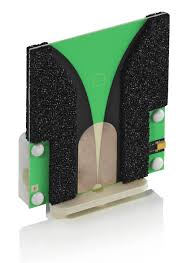
\includegraphics[width=\linewidth]{ProbeAntenna.jpg}
    \end{minipage}
    \caption{Specification of the Probe Antenna (\acs{RS}\textregistered{} - TS-F24-V2)}
\label{fig:probes}
\end{figure}      

\section{\ac{DUT}}
This thesis uses two DUTs (single antenna DUT and multi-antenna DUT) to investigate the measurement uncertainties introduced by conducted and normalized measurements. 

\begin{figure}[h]
    \begin{minipage}[c]{.7\textwidth}% or {.6\linewidth}, it's the same here
        \begin {tabular} {|l|l|} 
\toprule
Parameters & Value \\ 
\midrule 
Antenna type & detachable omni-directional \\
Antenna Gain & 3 dBi \\
Transmit Power & $<$ 20 dBm (\acs{EIRP})\\ 
Wireless Standards & \acs{IEEE} 802.11ac,a,n,g,b \\
Frequency & 2.4 and 5 GHz \\
\bottomrule
\end {tabular}    \end{minipage}
    \hfill
    \begin{minipage}[c]{.2\textwidth}
        \includegraphics[width=\linewidth]{SingleAntennaDUT.pdf}
    \end{minipage}
    \caption{Specification of the single-antenna \acs{DUT} (AC600 High Gain Wireless Dual Band USB Adapter, Archer T2UH)}
\label{fig:singleAntennaDUT}
\end{figure}     

\begin{figure}[h]
    \begin{minipage}[c]{.7\textwidth}% or {.6\linewidth}, it's the same here
        \begin {tabular} {|l|l|} 
\toprule
Parameters & Value \\ 
\midrule 
Antenna type & Omni-directional \\
Beamforming & Yes \\
Transmit Power &  $<$20 dBm (\acs{EIRP})\\ 
Wireless Standards & \acs{IEEE} 802.11ac,a,n,g,b \\
Frequency & 2.4 and 5 GHz \\
\bottomrule
\end {tabular}    \end{minipage}
    \hfill
    \begin{minipage}[c]{.2\textwidth}
        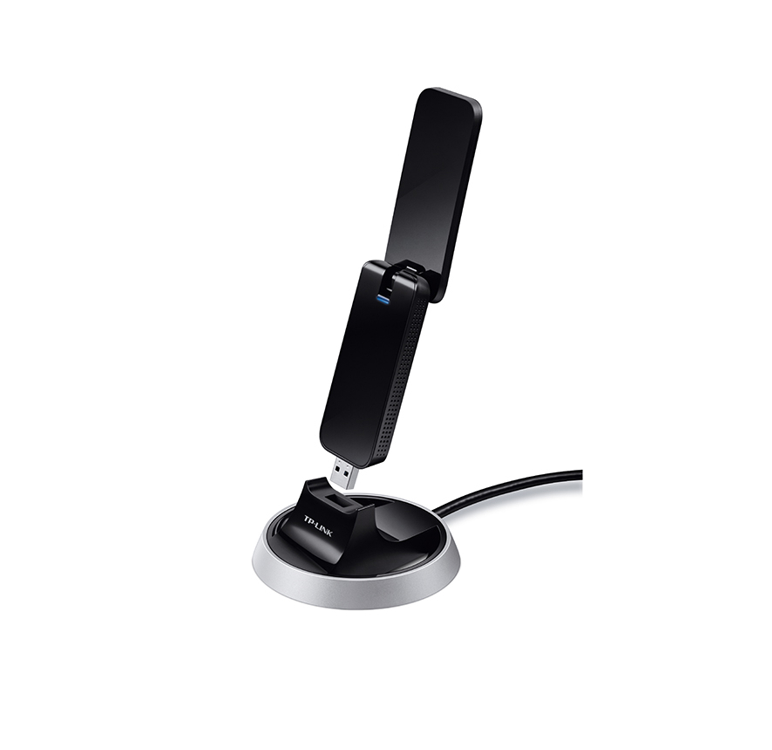
\includegraphics[width=\linewidth]{MultiAntennaDUT.pdf}
    \end{minipage}
    \caption{Specification of the multi-antenna \acs{DUT} (AC1900 High Gain Wireless Dual Band USB Adapter, Archer T9UH)}
\label{fig:multiAntennaDUT}
\end{figure}     

\chapter{Test Cases}\label{chap:test}

This thesis carries out tests for \acf{OBW} measurement, \acf{PSD} measurement, and Receiver Blocking measurement. The definition, limits and the procedure for each test case are mentioned in the subtopics below.

\section{\acl{OBW} measurement}
\label{sec:obw}

The \acf{OBW} is the bandwidth that contains 99 \% of the power of the signal. The standard EN 300328 mentions that the \acf{OBW} shall fall completely within the band (Table \ref{tab:bands}) for all types of equipment using wideband modulations other than \acs{FHSS}.  Besides, the limit shall be less than 20 MHz for non-adaptive equipment using wideband modulations other than \acs{FHSS} and with \acs{EIRP} greater than 10 dBm.

\begin{table}[ht]
\begin{center}
\begin {tabular} {|c|c|} 
\toprule
Function & Service frequency bands \\ 
\midrule 
Transmit & 2400 MHz to 2483.5 MHz \\
Receive & 2400 MHz to 2483.5 MHz \\
\bottomrule
\end{tabular} 
\caption{Service frequency bands}
\label{tab:bands}
\end{center}
\end{table}
The methodologies for this measurement are as follows:
\begin{enumerate}
  \item Associate the \acs{DUT} with the companion device. This step is explained in section \ref{sec:cmw}.
   \item Enable the Packet Generator with \acs{ICMP} or also known as ping packets. The companion device (\acs{RS}\textregistered{} wireless connectivity tester) supports the generation of \acs{ICMP} echo requests (ping) packets. These packets are targeted at the \acsp{DUT} \acs{IP} stack. Ping operates by sending \acs{ICMP} echo request packets to the \acs{DUT} and waiting for an \acs{ICMP} echo reply back. The \acs{DUT} is expected to answer with a well-defined echo reply packet whose payload is identical to the payload of the corresponding request. These packets are generated so that the bandwidth of the \acs{DUT} signal can be measured. Pinging triggers the \acs{DUT} to transmit a burst of a certain length which is useful for combined signal path measurements.

\textbf{image of ping packet}


\item Change the settings of the spectrum analyzer. The table \ref{tab:analyzer} below contains important analyzer settings.
\begin{table}[H]
\begin{center}
\begin {tabular} {|c|c|} 
\toprule
Function & Value \\ 
\midrule 
Center frequency & The centre frequency of the channel under test \\
Frequency span &2 $\times$ Nominal Channel Bandwidth \\
\ac{RBW} & (Span / 100) + 100e3 \\
\ac{VBW} & (3 $\times$ RBW) + 500e3\\
Time on each sweep point & 0.05 sec\\
Sweep points & ((2 $\times$ Span) /RBW + 1) $\times$ 10\\
Sweep time & Time on each sweep point $\times$ Sweep Points \\
Trace mode & Clear / Write\\
Detector & \ac{RMS}\\
\bottomrule
\end{tabular} 
\caption{Spectrum Analyzer settings for \ac{OBW} measurement}
\label{tab:analyzer}
\end{center}
\end{table}
The sweep time of 10 seconds is used instead of 1 second which is mentioned in the standard. This is because of the low duty cycle. There is nothing wrong with the standard, but by increasing the sweep time produces a better result that is more stable and reproducible. The standard suggests setting the trace mode to Max-Hold and then waiting for the trace to stabilize. Another way to stabilize the trace when the duty cycle of the signal is small is by using the trace mode as Clear / Write and increasing the sweep time.

\item Find the \ac{OBW}. This is well explained in the Figure \ref{fig:tracebw}.
\begin{figure}[H]
\centering
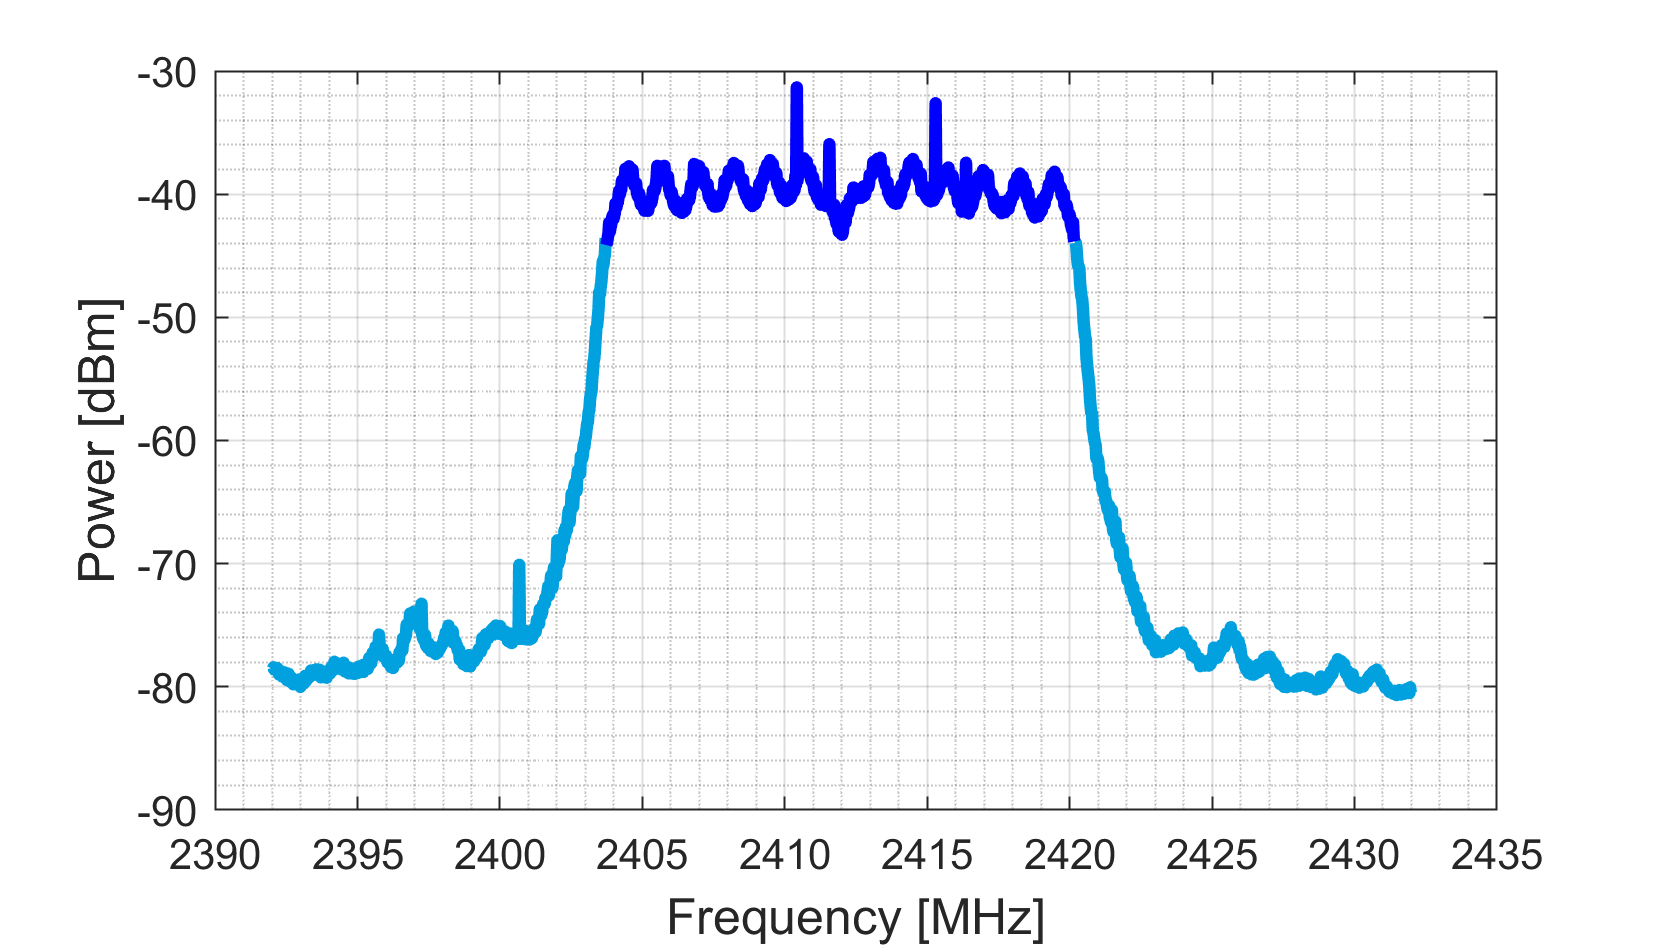
\includegraphics[width=0.65\textwidth]{TraceBandwidth.png}
\caption{Trace of the signal from the analyzer after post processing. The \acs{OBW} is 99\% (dark blue) of the total bandwidth of the signal}
\label{fig:tracebw}
\end{figure}
To locate the occupied channel bandwidth of the signal from the trace produced by the analyzer, we first convert the power value to a linear scale and find the total power. Since we need 99\% of the power, we go in a loop from both sides of the signal (start and stop frequency) and find the value of the frequency on both sides when the power value is 0.5\% of total power. And the difference between the frequency values gives us the 99\% occupied channel bandwidth.
\end{enumerate}
  
\section{\acl{PSD} measurement}
\label{sec:psdmeas}
The \acl{PSD} is the mean \acf{EIRP} spectral density in a 1 MHz bandwidth during a transmission burst. For equipment using wide band modulations other than \acs{FHSS}, the maximum \acf{PSD} is limited to 10 dBm per MHz. This test, like the occupied channel bandwidth measurement, requires the \acs{DUT} to transmit data so that the analyzer can save the trace for the calculation of \acf{PSD}. The steps for this measurement are as follows:

\begin{enumerate}
  \item Associate the \acs{DUT} with the companion device. Fritz Box acts as a companion device for this measurement. 
\item Run the batch (.BAT) file on the computer connected to the \acs{DUT}. This file uploads data to the \ac{NAS} which is connected to the USB stick on the companion device so that the power spectral density of the \acs{DUT} signal can be measured. Refer section \ref{sec:golden} for the procedure.
\item Change the settings of the spectrum analyzer. The table \ref{tab:analyzerpsd} below contains important analyzer settings.
\begin{table}[H]
\begin{center}
\begin {tabular} {|c|c|} 
\toprule
Function & Value \\ 
\midrule 
Start frequency & 2400 MHz \\
Stop Frequency  & 2483.5 MHz\\
\ac{RBW} & 10 KHz \\
\ac{VBW} & 30 KHz\\
Sweep points & 8500 \\
Channel Occupancy Time & 10 ms \\
Sweep time & Time on each sweep point $\times$ Sweep Points \\
Trace mode & Max-Hold \\
Detector & \ac{RMS}\\
\bottomrule
\end{tabular} 
\caption{Spectrum Analyzer settings for \ac{PSD} measurement}
\label{tab:analyzerpsd}
\end{center}
\end{table}
The standard suggests the number of sweep points to be greater than 8350. If the analyzers are not supporting this number of sweep points then the frequency band may be segmented. The measurement device used supports maximum of 15000 sweep points, but sweep points was set to 8500 in this case. Our aim being to reduce \acf{MU}, the sweep count is increased to 10 rather than using a single sweep. The maximum value of trace is saved with the help of Max-Hold trace mode.
  
\item Since the signal from the \acs{DUT} is non-continuous, wait for the trace to stabilize and save the trace data to a mat file.
 
 \item Use the following formula to add up the values of power for all sample points.
  $$ P_{sum} = \sum_{n=1}^{k} P_{sample}(n) $$ where k is the total number of samples and n is the actual sample number
  
 \item  Convert the power values from mW scale to dBm scale and then normalize the individual values for power so that the sum is equal to the \acs{RF} Output Power (\acs{EIRP}) measured in the big anechoic chamber and finally save the corrected data. The following formulas can be used:
  $$C_{corr} = P_{sum} - P_{EIRP}   $$ 
  $$P_{samplecorr}(n) = P_{sample}(n) - C_corr $$ where n is the actual sample number.
  
  \item Starting from the first sample $P_{samplecorr}(n)$ (lowest frequency), sum up the power (in mW) of the following samples representing 1MHz segment and record the results for power and position (i.e. sample 1 to sample 100). This is the Power Spectral Density (\acs{EIRP}) for the first 1 MHz segment.
  
  \item Shift the starting point of the samples by one sample summed up in step 7 and repeat the procedure in step 8. (i.e. sample 2 to sample 101)
  
  \item Repeat step 8 until the end of the data set and record the Power Spectral Density values for each 1 MHz segments. From all the recorded results, the highest value is the maximum Power Spectral Density of the \acs{DUT}. This value shall be recorded in the test report.
    \end{enumerate}
  
 \begin{figure}[H]
\centering
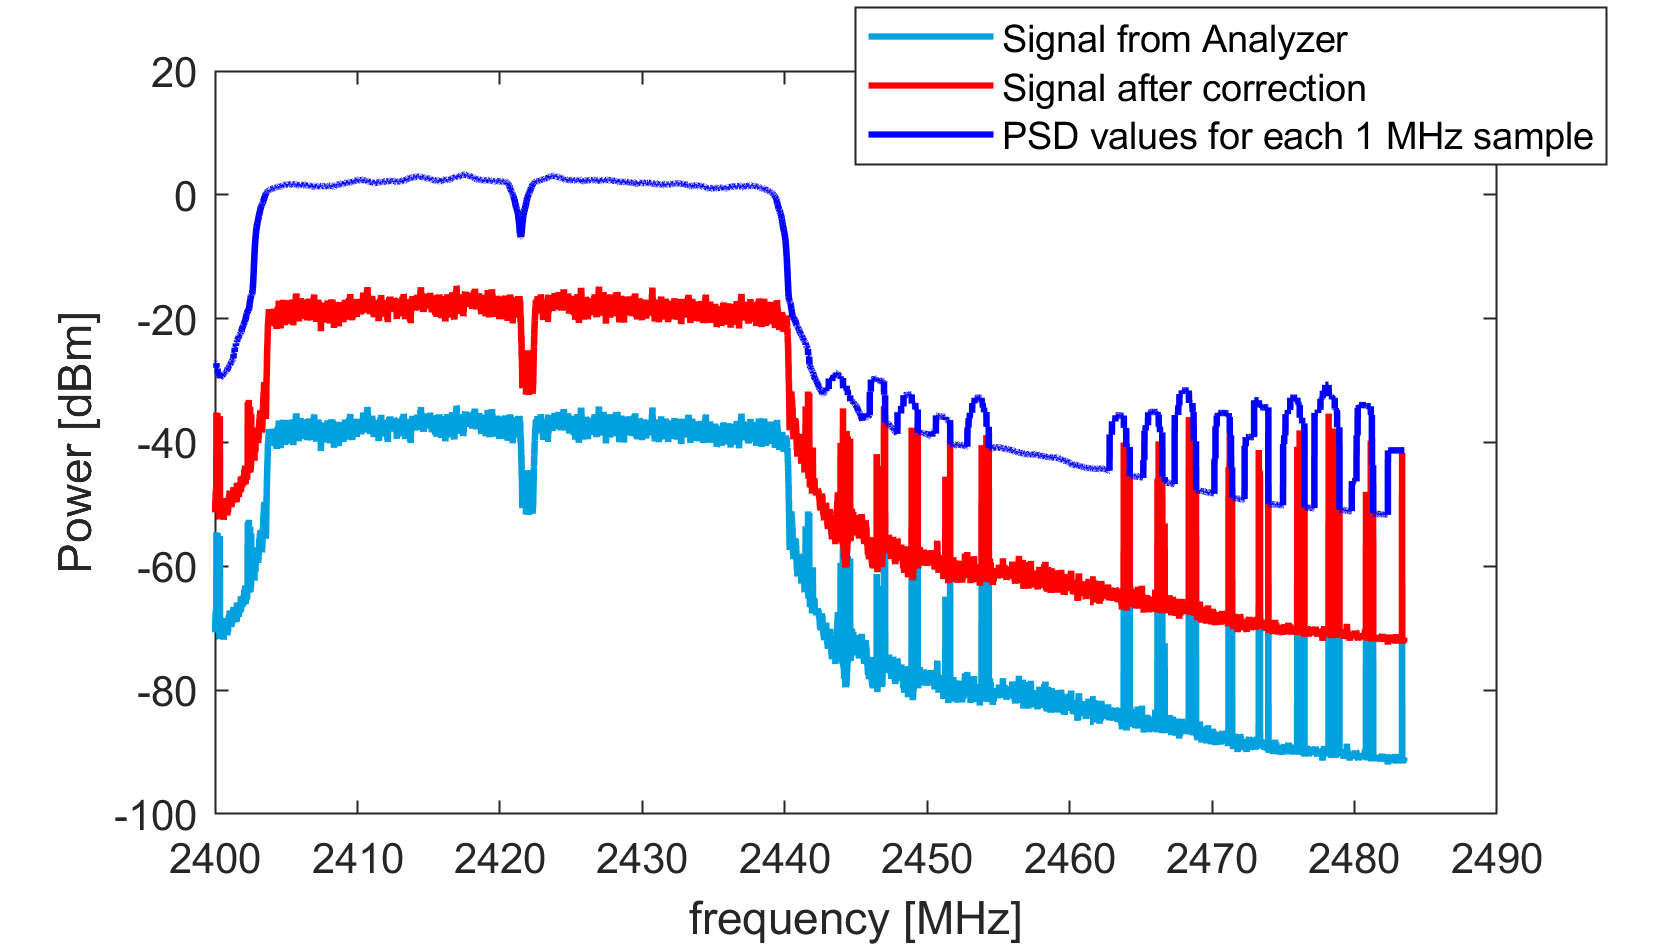
\includegraphics[width=0.75\textwidth]{PSD_trace.png}
\caption{Trace of the signal from the analyzer after post processing. The \acs{PSD} is 3.3015 dBm at 2418 MHz}
\label{fig:psdtraceI}
\end{figure}
  
  
 \section{Receiver Blocking measurement}
\label{sec:rxmeas} 
Receiver blocking is a measure of the ability of the equipment to receive a wanted signal on its operating channel without exceeding a given degradation in the presence of an unwanted signal (blocking signal) at frequencies other than those of the operating band. The minimum performance criterion shall be a \ac{PER} less than or equal to 10 \%. The manufacturer may declare alternative performance criteria as long as that is appropriate for the intended use of the equipment. The procedure for this measurement is explained in the Figure \ref{fig:flowchartrxvlock}.

 \begin{figure}[H]
\centering
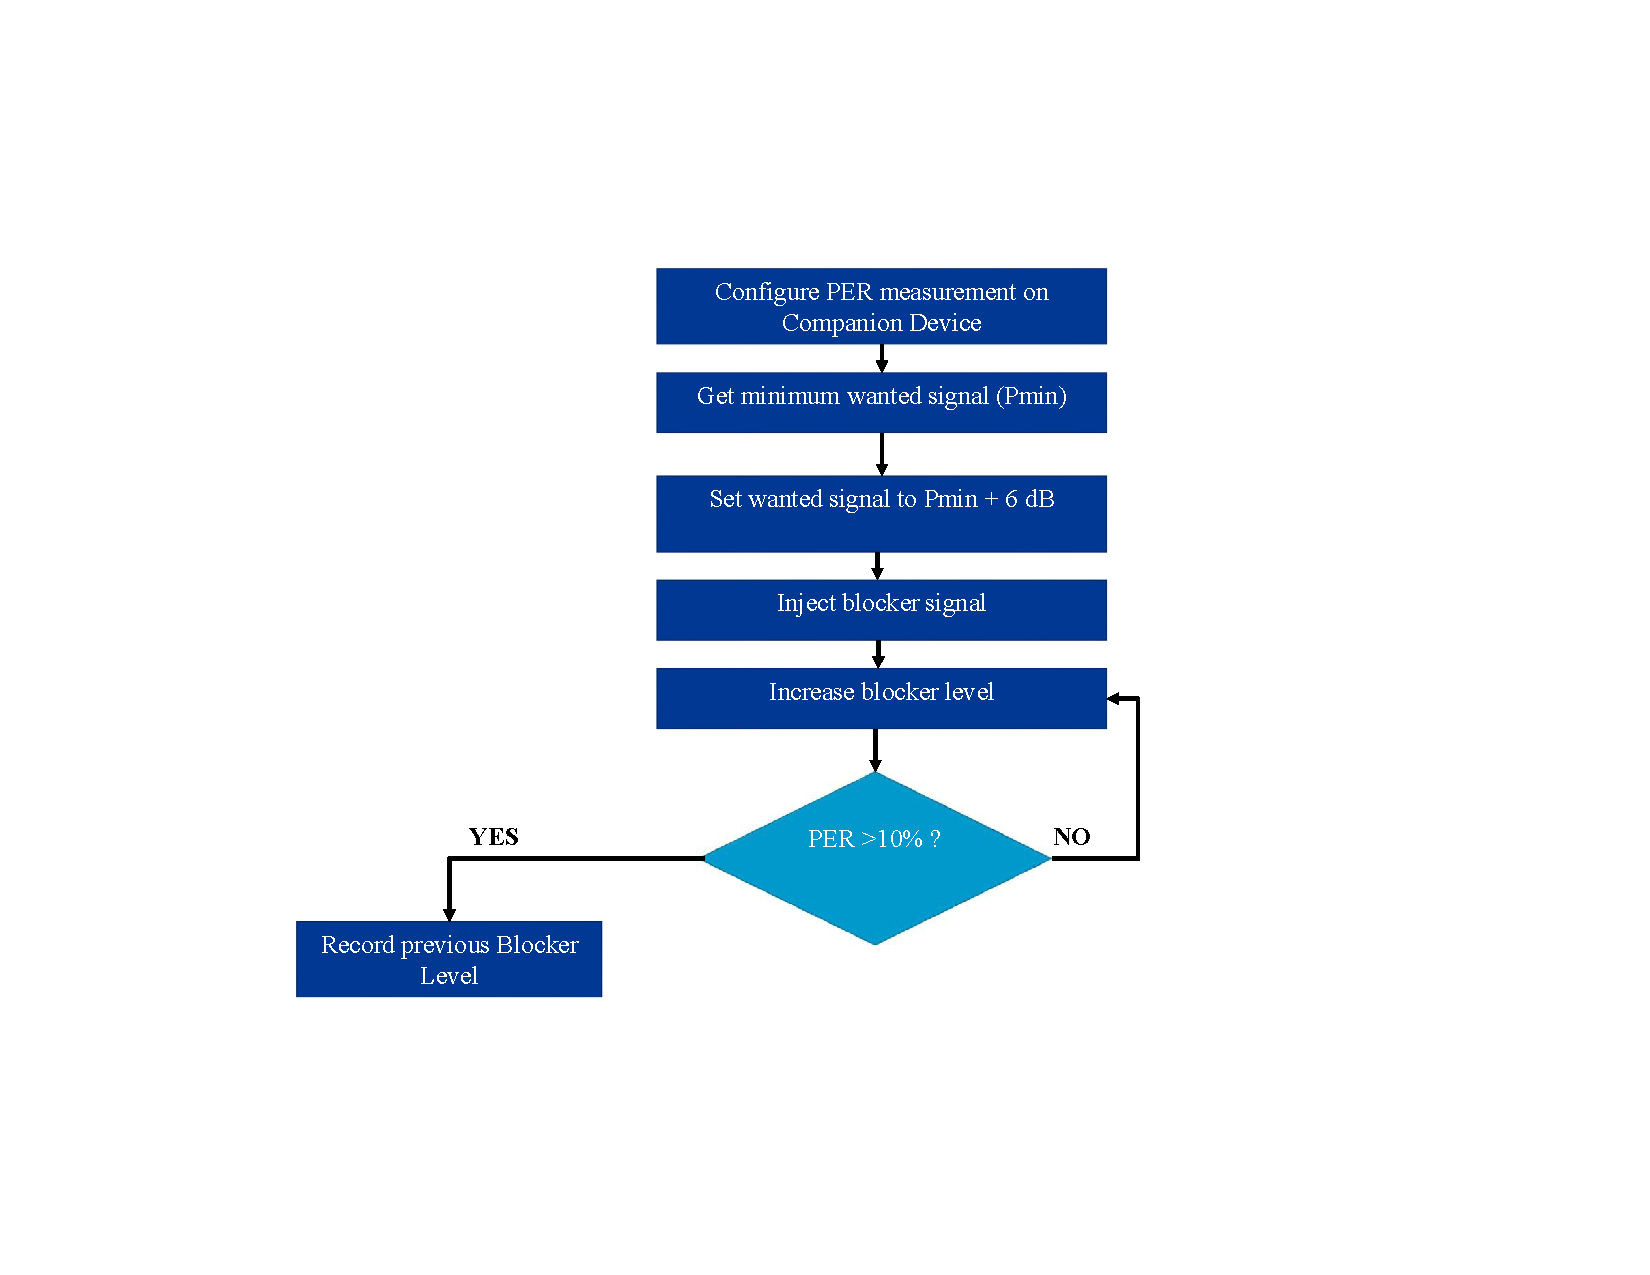
\includegraphics[width=0.9\textwidth]{flowchart.pdf}
\caption{Flowchart for Receiver Blocking measurement}
\label{fig:flowchartrxvlock}
\end{figure}

The association of the \acs{DUT} with the companion is talked about in all other test procedures as well as in the previous chapter. A \acf{PER} measurement is configured on the companion device. The \acs{PER} measurement transmits user data to the \acs{DUT} and calculates the \acs{PER} of acknowledged packets to transmitted packets. The number of MAC test packets to be transmitted is configurable. Each of the test packets carries the same amount of user data to the \acs{DUT}. The test packets can be separated by unused packets. The diagram in the lower part of the dialog shows the \acs{PER} vs time/transmitted packets.

 \begin{figure}[H]
\centering
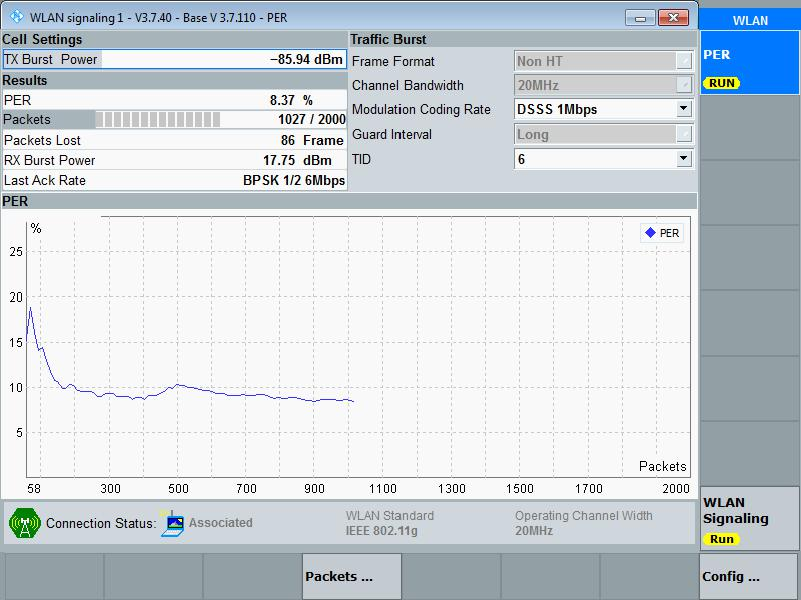
\includegraphics[width=0.75\textwidth]{PER_CMW.jpeg}
\caption{\ac{PER} measurement on the \acs{RS} \acs{CMW}}
\label{fig:per}
\end{figure}

The next phase is to find the minimum wanted signal ($P_{min}$) without the blocker (signal generator). To do this, the power of the transmitted bursts is kept reducing until the \acs{PER} reaches just below 10\%. In order to increase the speed of the measurement, the program first does coarse precision (i.e. reduces power by steps of 1 dBm and sets the transmitted packets to as low as 200). Then for precise measurement, the power is reduced in steps of 0.1 dBm and 2000 packets are transmitted. The \acs{PER} window in the figure above shows the \acs{PER} measurement taking place. \\
  
This is followed by keeping the wanted Signal ($P_{min}$ + 6 dB) constant and injecting a blocker signal using a signal generator at the frequency mentioned in the standard. \acs{PER} measurement then checks for the resulting \acs{PER}. The blocking signal of -34 dBm is applied in front of the \acs{DUT} as mentioned by the standard. Then, the transmitted burst power is kept constant thought-out the measurement by adding 6 dBm to the minimum unwanted signal. The blocker level is kept increasing until the 10\% criterion is reached. This is not required by the standard but it shows us by how much we can take the power level above the value mentioned in the standard. It also gives us an impression of how good the \acs{DUT} performs and allows us to assess the \acf{MU}.





\chapter{Conducted Measurements} \label{chap:5}

The term Conducted Measurements refers to measurements performed using \acs{RF} cables connected between the antenna port of the \acs{DUT} and the instruments (off-air). Most \acs{WLAN} regulatory compliance mandate that conducted measurements shall be used for most compliance tests (transmit power, in-band spectrum density, bandwidth, and parts of the spurious scan) for a \acs{DUT} with antenna connector(s) and using a dedicated external antenna(s), or for a \acs{DUT} with integrated antenna(s) but with temporary antenna connector(s) provided \cite{conducted}. As mentioned in the chapter \ref{chap:test}, this thesis implements tests for \acf{OBW} measurement, \acf{PSD} measurement, and Receiver Blocking measurement.

\section{Using Attenuator and Splitter}
\label{sec:att}
Figures \ref{fig:Ng1} and \ref{fig:Ng2} show the block diagram of the connections of the instruments during conducted measurements. To not complicate things, the \acs{DUT} is connected via a Wi-Fi\texttrademark{} connection to a laptop. The \acs{DUT} in this case is a single antenna \acs{DUT} (Archer T2UH \ref{fig:singleAntennaDUT}). This \acs{DUT} is further associated with the \ac{CMW} (wireless connectivity tester). The companion device acts as an access point. The splitter is used to split a single \acs{RF} line into two different \acs{RF} lines. The attenuator of 20 dB is required to reduce the signal strength. When using a spectrum analyzer, the attenuator benefits by not allowing the spectrum analyzer to measure the power coming from the companion device. The light blue lines in the Figure \ref{fig:Ng1} and Figure \ref{fig:Ng2} indicate the signals for association of the \acs{DUT} with the companion.
\begin{figure}[H]
\centering
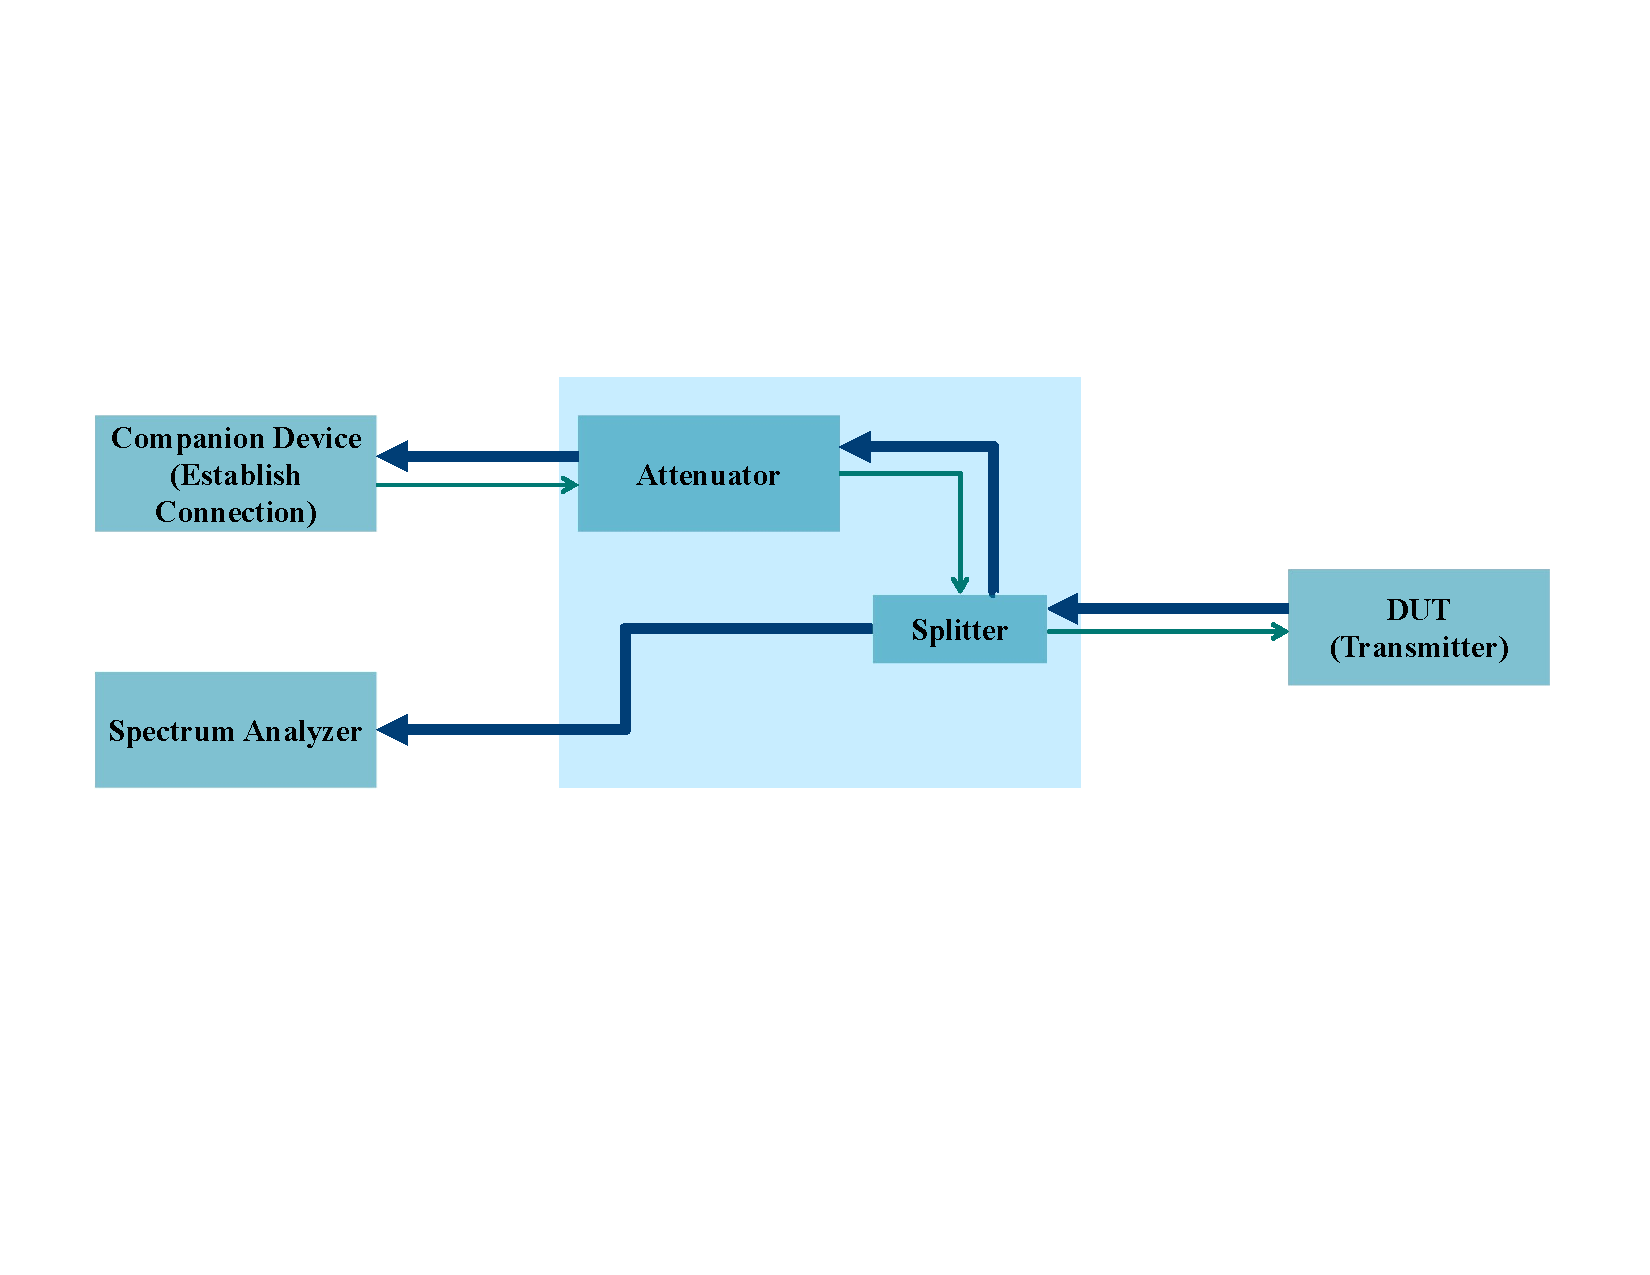
\includegraphics[width=0.9\textwidth]{conductedtx.pdf}
\vspace{-3.2cm}  \caption{Conducted measurements using attenuators and splitters: \acs{DUT} is assessed for its transmitter capabilities}
 \label{fig:Ng1} 
\end{figure}

The hardware setup shown in Figure \ref{fig:Ng1} performs the \acf{OBW} and \acf{PSD} measurement. The spectrum analyzer is used to measure the spectrum of the signal from the \acs{DUT} and then assess the \acf{OBW} or the \acf{PSD} based on this data. Since the \acs{DUT} behaves like a transmitter, most of the signal is going away from the \acs{DUT} (dark blue lines) but there is also some receiving when a connection is established between the \acf{CMW} and the \acs{DUT}. The approach to find 99\% of the \acf{OBW} and \acf{PSD} is explained in the section \ref{sec:obw}.

\begin{figure}[H]
\centering
   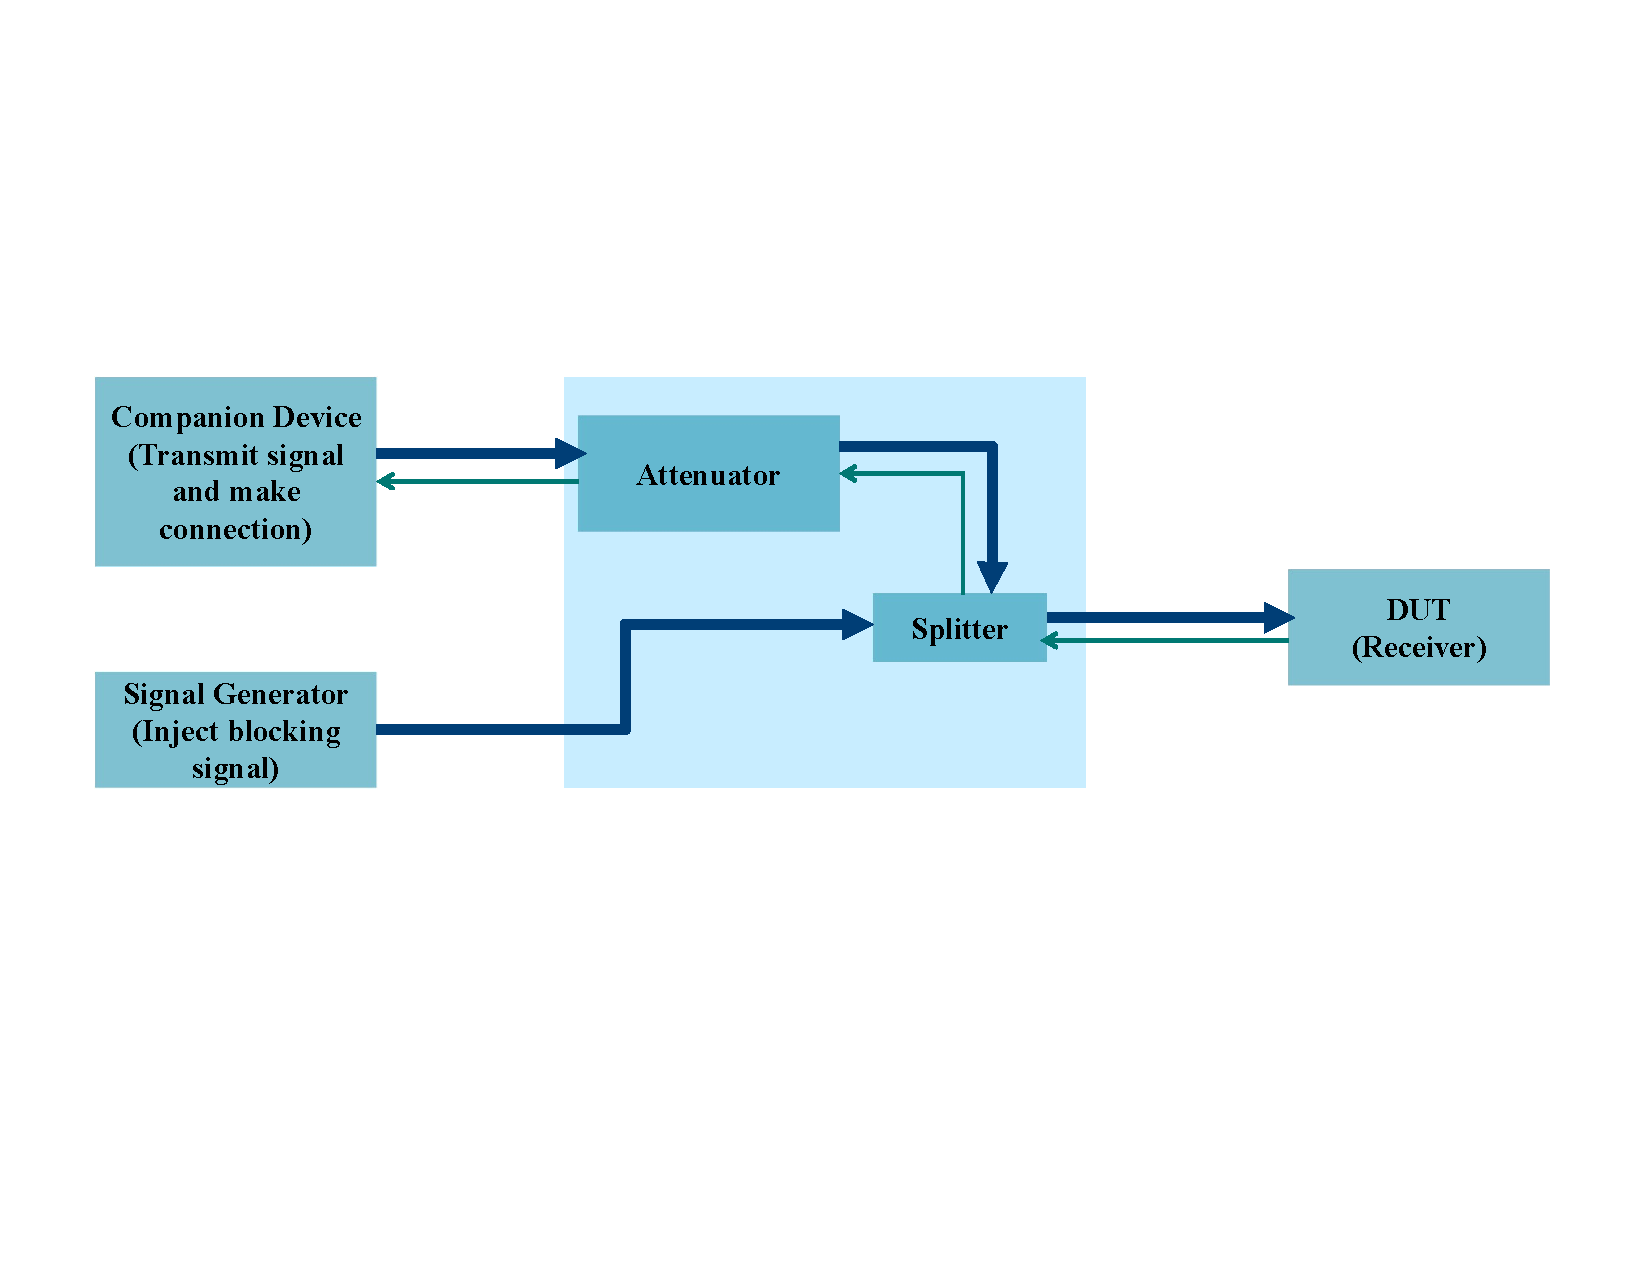
\includegraphics[width=0.9\textwidth]{conductedrx.pdf}
 \vspace{-3.2cm} \caption{Conducted measurements using attenuators and splitters: \acs{DUT} is assessed for its receiver capabilities}
   \label{fig:Ng2}
\end{figure}

When the \acs{DUT} acts as a receiver in Figure \ref{fig:Ng2}, the signal generator generates a blocking signal (unwanted signal) on the frequencies other than those of the operating band.  \acf{PER} measurement examines the ability of the \acs{DUT} to receive a wanted signal on its operating channel without exceeding 10\% degradation in the presence of a blocking signal. 

\section{Using a Switching Matrix}
\label{sec:switch}
The next goal is to use a dedicated switching matrix instead of changing splitters and attenuators for every test measurement. Before starting the measurement, the first step is to switch the correct paths within the switching modules required for the test. \\

For the receiver blocking test case, the blocker power level at the signal generator is calculated by adding the cable losses, attenuation from the switching units, and the antenna gain of the \acs{DUT} to the blocker power level mentioned in the standard. The formula to calculate the blocker level at the generator is shown in equation \ref{eq:1}:

\begin{equation}
\begin{aligned}
\mbox{BL}_ {\mbox{Gen}}  &= \mbox{BL}_ {\mbox{DUT}} + \mbox{ATT}_{\mbox{cables}} 
+ \mbox{ATT}_{\mbox{OSP}}  - \mbox{Gain}_{\mbox{ DUT}}
\label{eq:1}
\end{aligned}
\end{equation}
BL stands for blocker level, ATT for attenuation, and OSP for \acf{OSP}. For example, the standard mentions that at blocker frequency of 2380 MHz, the required blocker level in front of the \acs{DUT} is -53 dBm. Assume the total attenuation is 40 dB and the antenna gain of the \acs{DUT} is 3 dBi. Then,
$$\mbox{Blocker Level at the Generator} = -53 \mbox{dBm} + 40 \mbox{dB}- 3 \mbox{dBi} = -16 \mbox{dBm}$$ 
The results from Receiver Blocking and \acf{OBW} measurements are compared with the implementation in the WMS32 software suite. The results match and therefore the next step is to perform normalized measurements, which is explained in the chapter \ref{chap:normalized}.







\chapter{Normalized Measurements}\label{chap:normalized}
This chapter explains the procedure for normalized measurements. The first section gives a layout for both hardware and software implementation of the normalized measurements and is followed by a short explanation to \acs{EIRP} measurement. Then the next section defines the link-budget for this approach. The fourth section demonstrates the normalization procedure. Following this explains the optimization of the antenna pair. The final section illustrates the program for the selection of the best-required probe antennas.


\section{Implementation}
The flow chart in Figure \ref{fig:1} explains the procedure for normalized measurements. Each step in the flowchart is further explained in detail in the further sections of this chapter. For the normalization measurements, the first step is to find the \acs{EIRP} of the \acs{DUT}. This can be done by a conducted measurement or by simply measuring the \acs{EIRP} in an \acf{AC}. The later provides us with the radiation pattern of the \acs{DUT}.  The \acs{EIRP} measurement is just done once for each \acs{DUT} and the results are normalized using this \acs{EIRP} value of the \acs{DUT}. Before performing the normalized measurements, it is important to find the best configuration for the cables and connections. This step is also done only once and all other measurements are done using the same configuration of the instruments and cables. This step also includes the calibration of all the cables within the system.  The section \ref{sec:opti} explains the above procedure.

\begin{figure}[H]
\centering
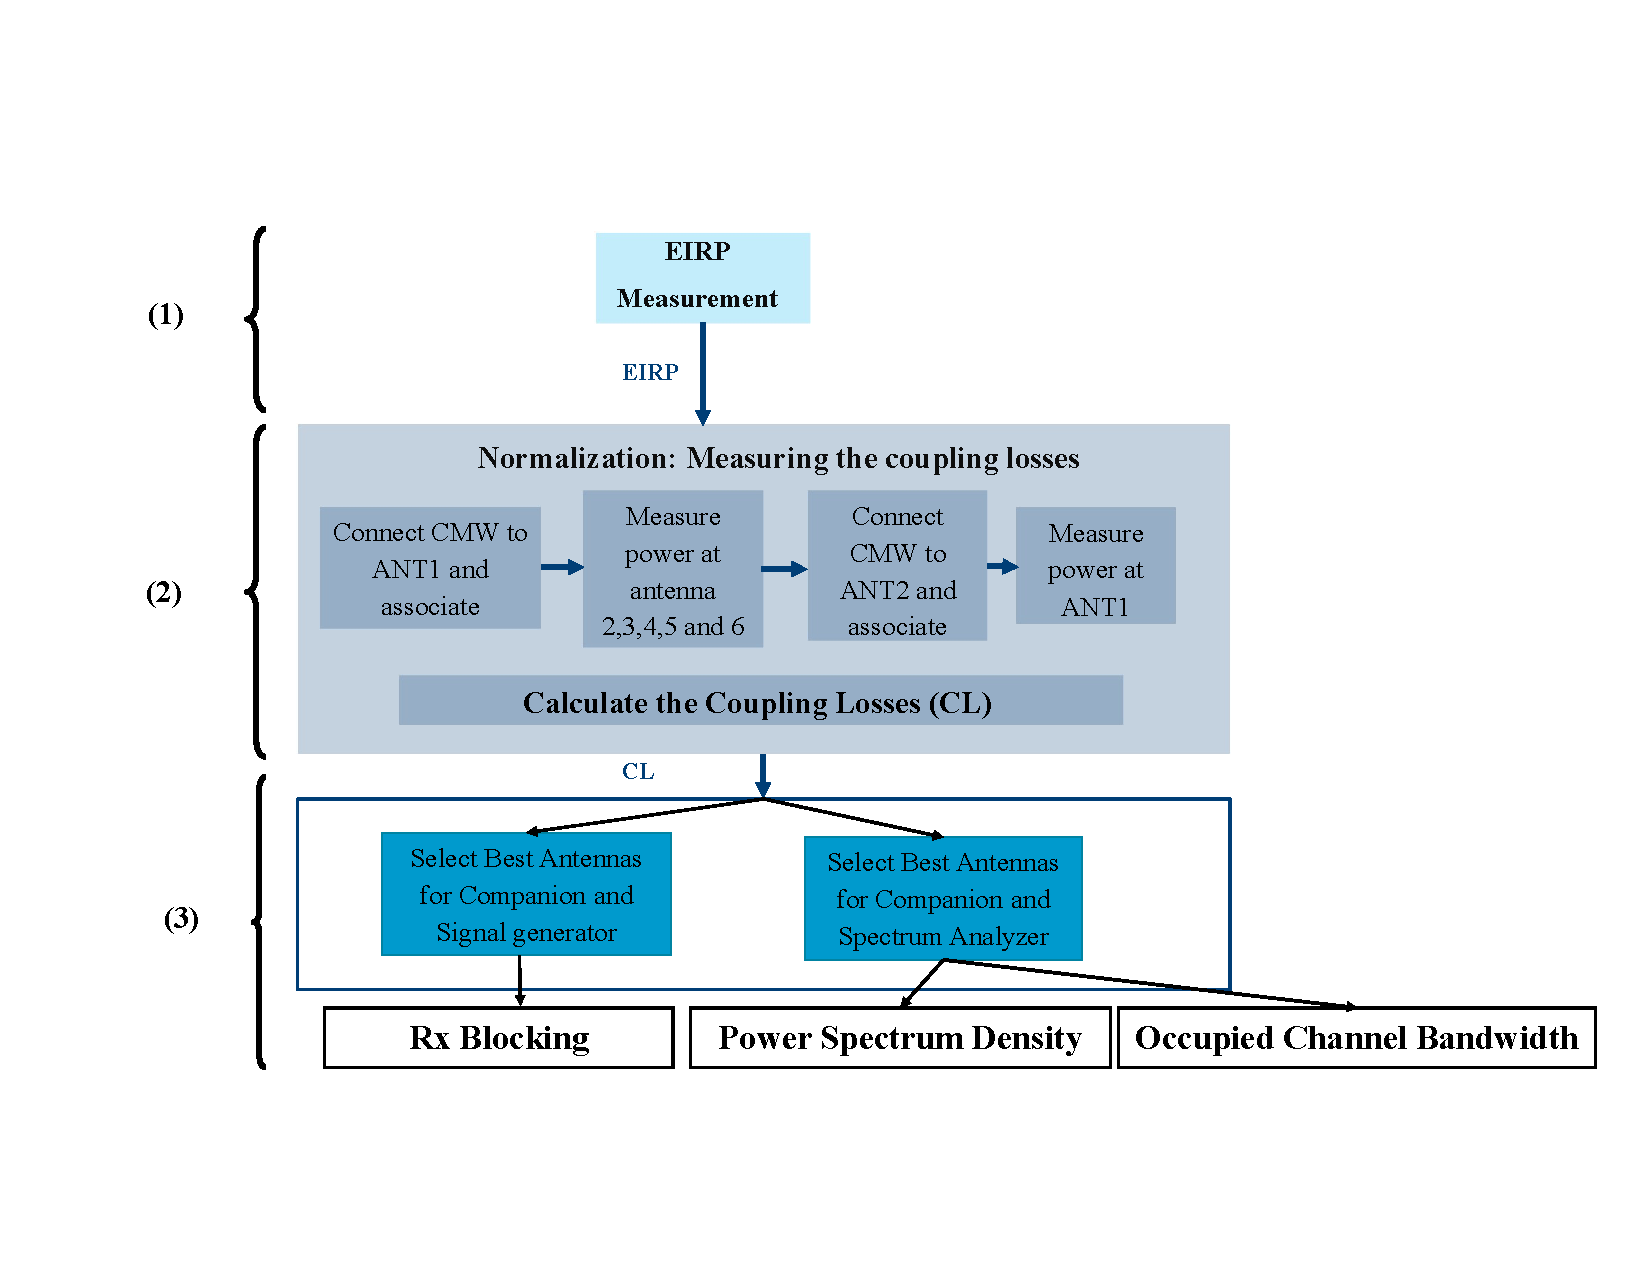
\includegraphics[scale = 0.6]{normflowchart.pdf}
\vspace{-2.2cm} \caption{Flowchart explaining the novel approach for wireless coexistence testing}
\label{fig:1} 
\end{figure}

The second block (2) in the flow chart \ref{fig:1} is explained in the section called Normalization. This procedure is vital for these measurements. This step is done every time a new test is run. Sometimes, long term measurements are done so that the \acf{MU} for the particular test case can be evaluated. This step then is performed at the beginning of the long term measurement and therefore the resulting coupling loss is used for all the measurement times during that long term measurement. \\
 
The selection of the best antenna probe depends mainly on the test case specification. For example, the companion device and the spectrum analyzer is used for \acf{OBW} measurement and \acf{PSD} measurement. And, the Receiver Blocking test case uses the companion device along with the signal generator. Each instrument usually is confined to 2 antenna ports due to the internal block diagram of the switching module (explained in section \ref{sec:wn}). The procedure for the selection is explained in the sub-topic called the selection of the best probe antenna. The measurement is run after all the mentioned steps. To get a good idea of the \acf{MU}, each test measurement is run several times, and the mean and standard deviation is computed. \\

This section also gives a brief overview of the implementation of the developed MATLAB\textregistered{} tool. The Figure \ref{fig:2} shows the individual steps of the measurement process implemented in this thesis.

\begin{figure}[H]
\centering
\includegraphics[scale = 0.6]{arrow.pdf}
\vspace{-2cm}\caption{Flow of the automation software}
\label{fig:2} 
\end{figure}

The software tool for automated wireless coexistence measurement is implemented in MATLAB\textregistered{} because of several reasons. MATLAB\textregistered{} is a numerical computing environment and fourth-generation programming language allowing matrix manipulations, plotting of acquired data, implementation, and testing of algorithms (e.g. for signal processing and antenna radiation patterns). One big advantage of MATLAB\textregistered{} is the availability of commonly used functions that are already implemented in the MATLAB\textregistered{} environment. Additionally, there are many toolboxes available, which are either free or can be purchased from MathWorks or third party suppliers. \acs{RS}\textregistered{} has many of these additional toolboxes licensed, which reduces development time significantly. This is especially important when studying new approaches as in the case of this thesis.

\subsection{Hardware Design}
The steps for implementation of radiated measurements are explained as follows:
\begin{enumerate}
  \item Place the \acs{DUT} inside an \acf{AC} and measure the maximum \acs{EIRP} from the \acs{DUT}.
  \item Place the \acs{DUT} in the \acs{RF} shielded box and connect the instruments as shown in the block diagram.

\begin{figure}[H]
\centering
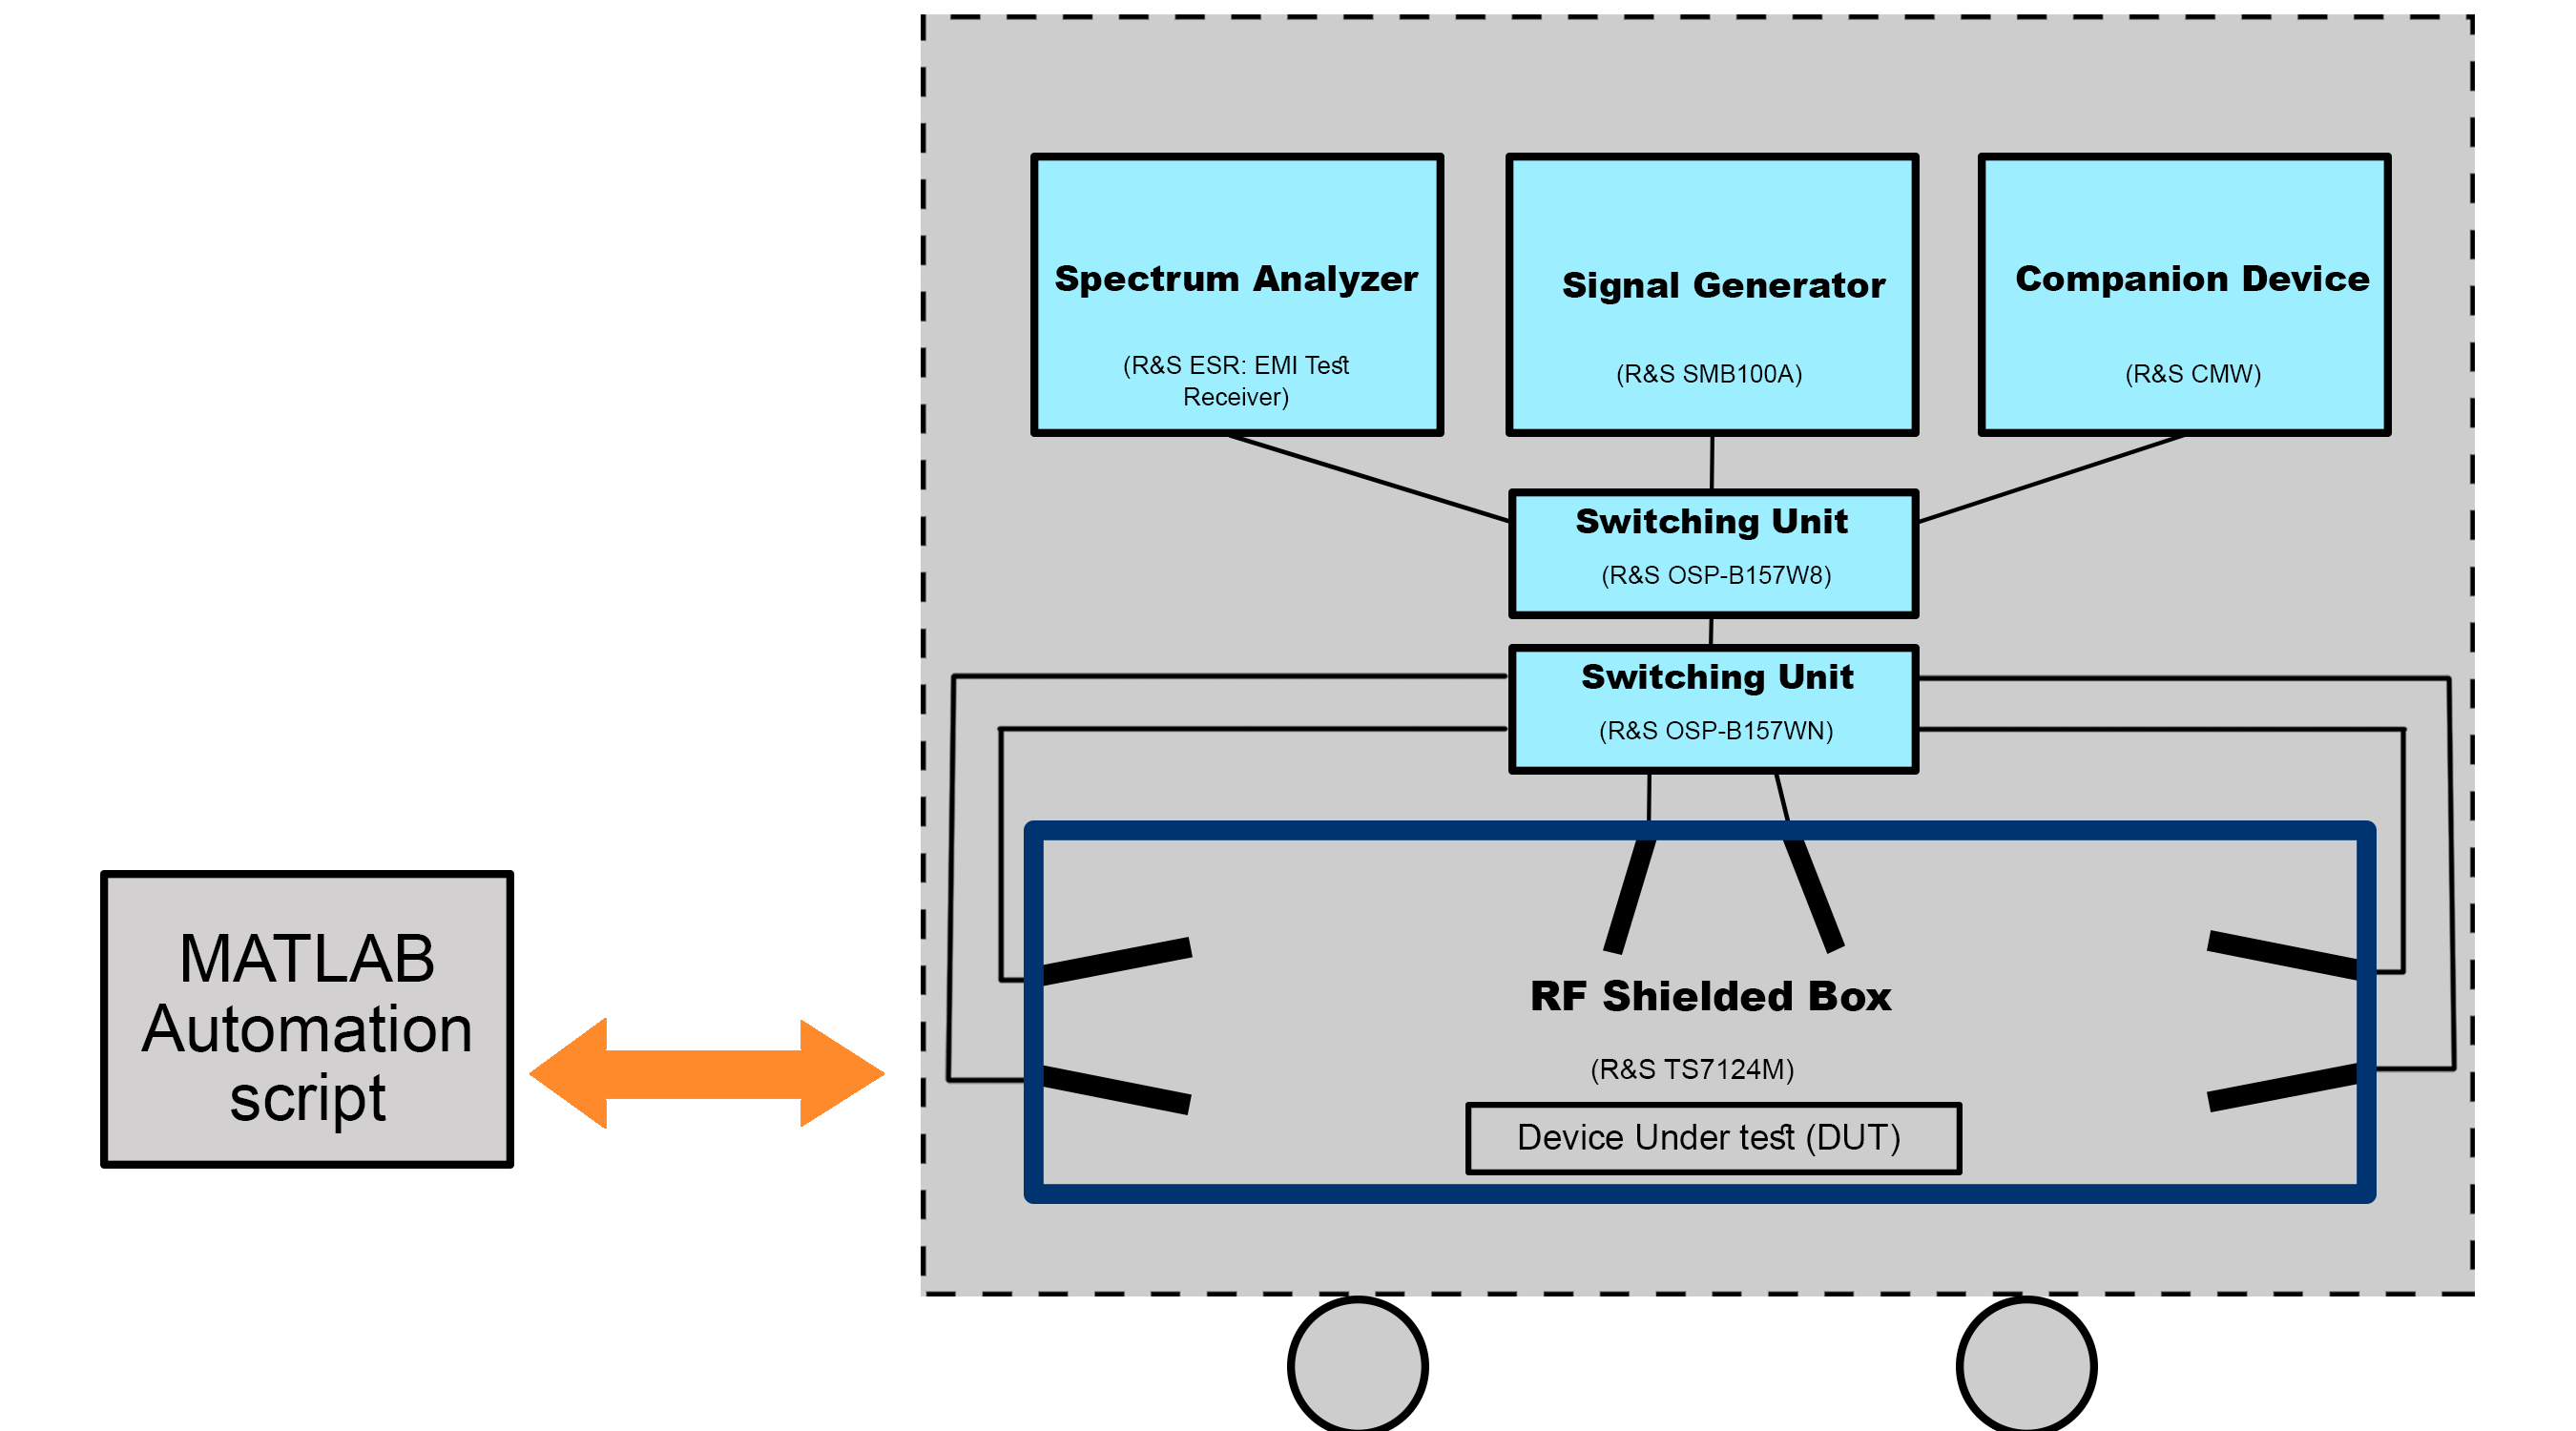
\includegraphics[scale = 0.18]{hwdesign.png}
\caption{Design for the implementation of the wireless coexistence system}
\label{fig:3} 
\end{figure}

There are six probe antennas inside the \acs{RF} shielded box. They work in pairs of 2. i.e. 2 antennas for spectrum analyzer which is used for measuring the power, bandwidth, etc. 2 other antennas are used for injecting a signal which is used in case of receiver blocking or adaptivity test case. And finally, the last pair of antennas are used for communicating with the \acs{DUT} by the companion device.

\item Perform Normalization: Power, which is found by calculating the average of each burst of the \acs{DUT} signal and finding the maximum of all bursts, is measured at all six antennas. The difference between the measured \acs{EIRP} in step 1 and the power measured at each antenna is defined as the coupling loss for that particular path. This step is explained in detail in the next section.

\item Select the best probe antenna out of each pair of antennas depending on the different test cases. The best probe antenna is considered the one which has minimum coupling loss. This step is explained in section \ref{sec:sba}. 

\item Run a measurement from the decided test cases. The procedure for each test case is explained in chapter \ref{chap:test}.

\end{enumerate}



\subsection{Software Design}
After the conducted measurement analysis was fundamentally verified in the experimental setup, the software implementation was restructured. Since the complexity of the implementation grew over time, an object-oriented programming style is used in the current implementation to account for this development. The object-oriented design improves the understanding of the code because the structure represents the real nature of the data well.

When one creates a class in MATLAB\textregistered{}, it is by default a value class. I prefer having to update objects by reference, therefore the class uses a handle class. This can made a handle class by changing the first line to:
\begin{lstlisting}[language=MATLAB]
classdef testClass < handle
\end{lstlisting}
Also, one wouldn't necessarily need output arguments for the methods of the handle class which is one of the main reasons for using this class. \\

The seven classes build the core of the developed software tool . For better overview and understanding some attributes and methods are omitted in this class diagram (Figure \ref{fig:cd}). Each of these classes is derived from the base class Handle. The CAutomation class instantiates objects from all the other six classes. Five of those classes are the instruments used in this thesis, i.e., Spectrum Analyzer, Signal Generator, Connectivity Tester, two Switching modules, and the last class named CDUT, specifies the \acs{DUT} standard, operating frequency, bandwidth, \acs{EIRP}, and so on.

\begin{figure}[H]
\centering
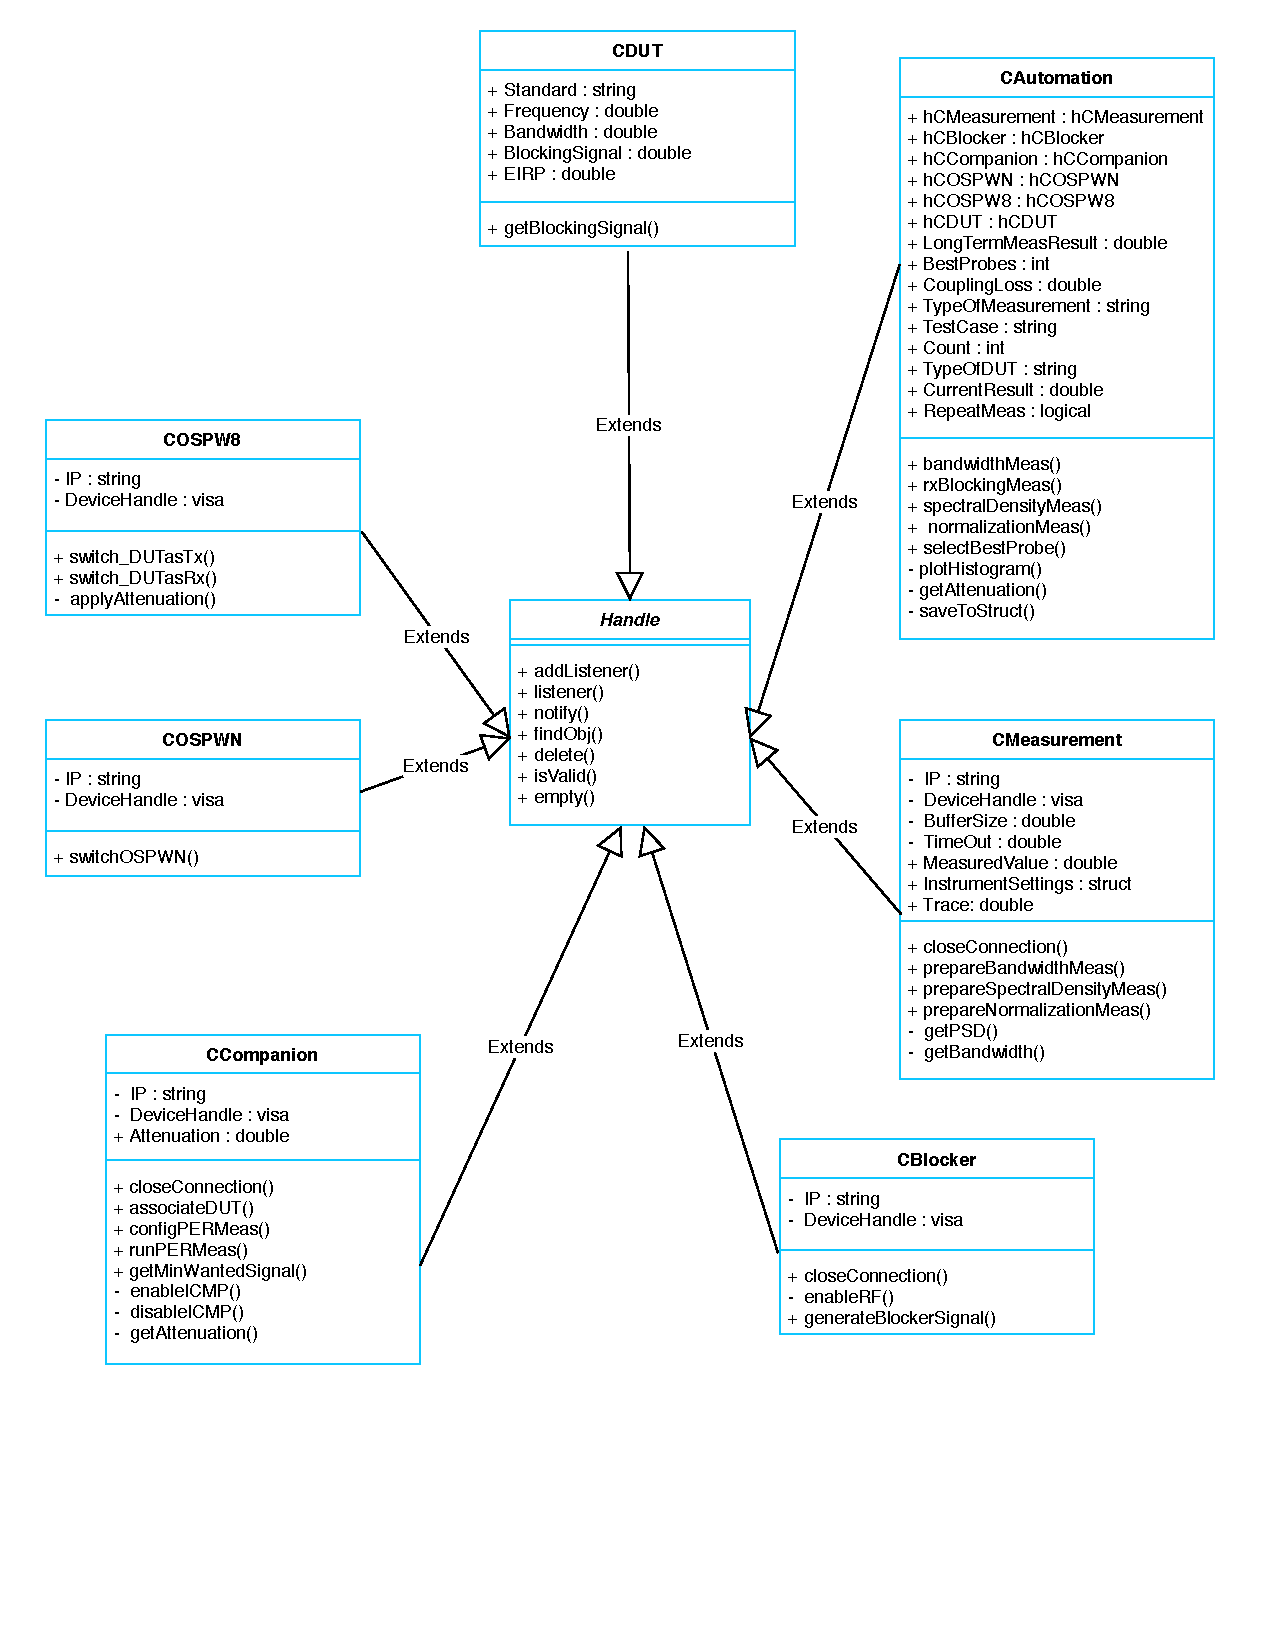
\includegraphics[scale = 0.75]{ClassDiagram.pdf}
\caption{UML Class Diagram}
\label{fig:cd} 
\end{figure}



\section{\acs{EIRP} Measurement}
\acs{EIRP} is measured once for every \acs{DUT} used. Maximum \acs{EIRP} is generally measured using \acs{OTA} measurements.  But, in this case the \acs{EIRP} estimation is done by measuring the conducted output power and applying the stated antenna gain. The Figure \ref{fig:Ng1} explains the implementation of this measurement. The \acs{DUT} is associated with the companion device via a \acs{WLAN} signaling mode. The \acs{DUT} is set to transmitter mode by configuring \acs{ICMP} packets on the companion device. The spectrum analyzer therefore, measures the power of the signal from the \acs{DUT}. The \acs{EIRP} is then measured using the formula \ref{eq:eirp}.
\begin{equation}
\mbox{EIRP}  = \mbox{Power}_{\mbox{analyzer}} - \mbox{Attenuation}_{\mbox{cable}} + \mbox{Antenna Gain} \label{eq:eirp}
\end{equation}
This measurement can also be done in an \acf{AC} and would give a better result by providing us the radiation pattern of the \acs{DUT} antenna.


\section{Normalization} \label{sec:11}
Normalization aims at finding the coupling loss at each antenna port. This data further aids in finding the best probe antenna. The steps for normalized measurement is explained as follows:
\begin{enumerate}
\item As mentioned in the section \ref{sec:wn}, the companion device (wireless connectivity tester) is connected to the COMP1 port of the OSPWN. Therefore, switch the path between ANT1 and COMP1 and establish a \acs{WLAN} connection between the two devices (\acs{DUT} and the \acs{CMW}). 
\item Configure the Packet Generator (explained in section \ref{sec:obw}) on the companion device to measure the signal from the \acs{DUT}. This thesis focuses on using the CMW as a companion device but this will also work for using other companion devices (e.g. Access Point).
\item Switch paths in a loop: ANT 2 to OUT2, ANT 3 to OUT 3, and so on (refer to Figure \ref{fig:ospwn}). Save the trace of the signal for each path from the \acs{DUT} by using the spectrum analyzer. Thus, we get the traces for ANT 2 to ANT5 ports.
\item To measure the signal at ANT1, switch path ANT2 to COMP1 and save the trace at ANT1. Attenuation for each path inside each switching module is taken from the calibration files provided with the switching modules. The coupling loss is measured using the equation \ref{eq:bl}.
\begin{equation}
\mbox{Power}_{\mbox{analyzer}}  = \mbox{EIRP} - \mbox{Coupling Loss} - \mbox{Attenuation}_{\mbox{total}}  \label{eq:bl}
\end{equation}
\end{enumerate}
The total attenuation comprises attenuation within the switching modules as well as the attenuation from the cables. The coupling loss accounts for the free space path loss, antenna gain, and polarization mismatch. The post-processing required to measure the power from the trace acquired at the spectrum analyzer and the link budget to calculate the power required at the signal generator is explained with the help of an example in the following sub-section \ref{sec:abc}.

\subsection{Post Processing for Power measurement} \label{sec:abc}
The \acs{DUT} is actually transmitting signals as bursts and the standard mentions that burst power is the limit for the power measurements. This is also the reason why we use burst power detection also for the \acs{EIRP} measurement in an \acf{AC}. And therefore, also use it for normalization to calculate the coupling loss. \\

For each power measurement for each antenna, 20 traces are saved. The measurement is done in the time domain (i.e. zero span) because a single frequency is of interest to us and also due to the very low duty cycle of the signal from the \acs{DUT}. The purpose of the zero span is to specifically turn off the sweep function, as the sweep sometimes really ruin the measurement. If you have a pulsed source, if the pulse happens when the sweep is not on that one frequency, it misses the pulse power.\\

Each trace is as short as 20 ms. For each trace, the maximum power is found by taking the maximum of the average of each burst. Short trace is used because if the sweep time was increased e.g. to 100 ms then, there would be fewer points per burst to take an average. Since the sweep points considered are already maximum (32000), the only option remaining is to reduce the sweep time so that a better average can be done.  

\begin{figure}[H]
  \centering
  \subfigure[Sweep time of 100ms]{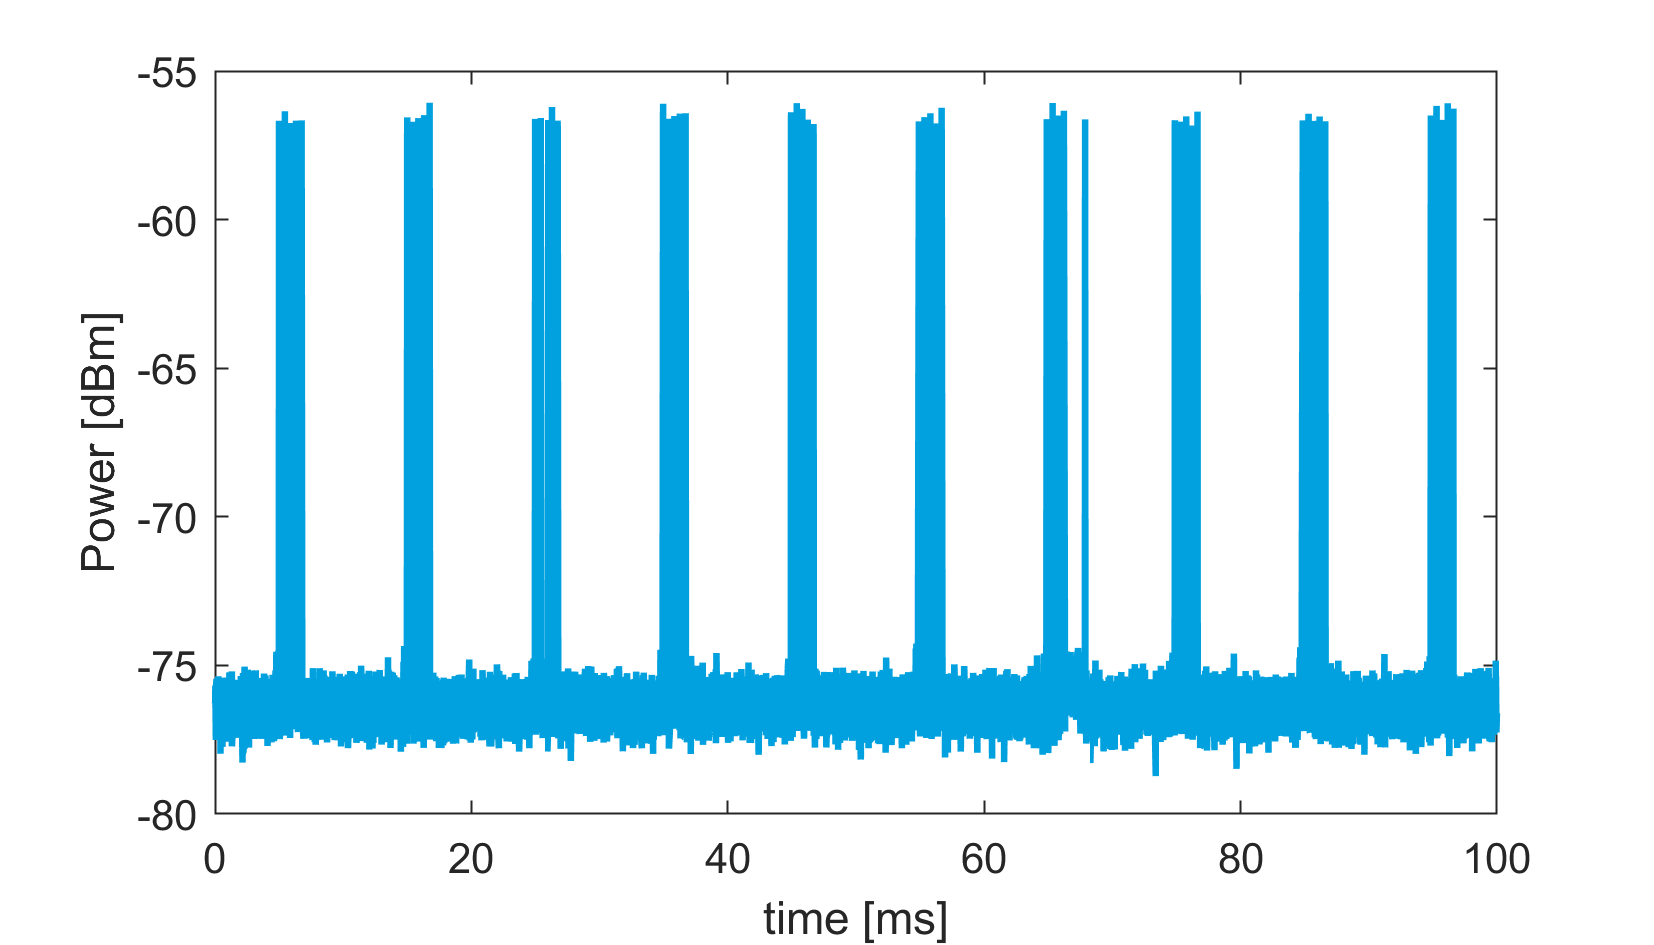
\includegraphics[width=0.49\textwidth]{trace_100.png}} \label{fig:m}
  \centering
  \subfigure[Zoomed trace of Figure (a)]{\includegraphics[width=0.49\textwidth]{{trace_100_zoom.png}}} \\
   \subfigure[Sweep time of 20ms]{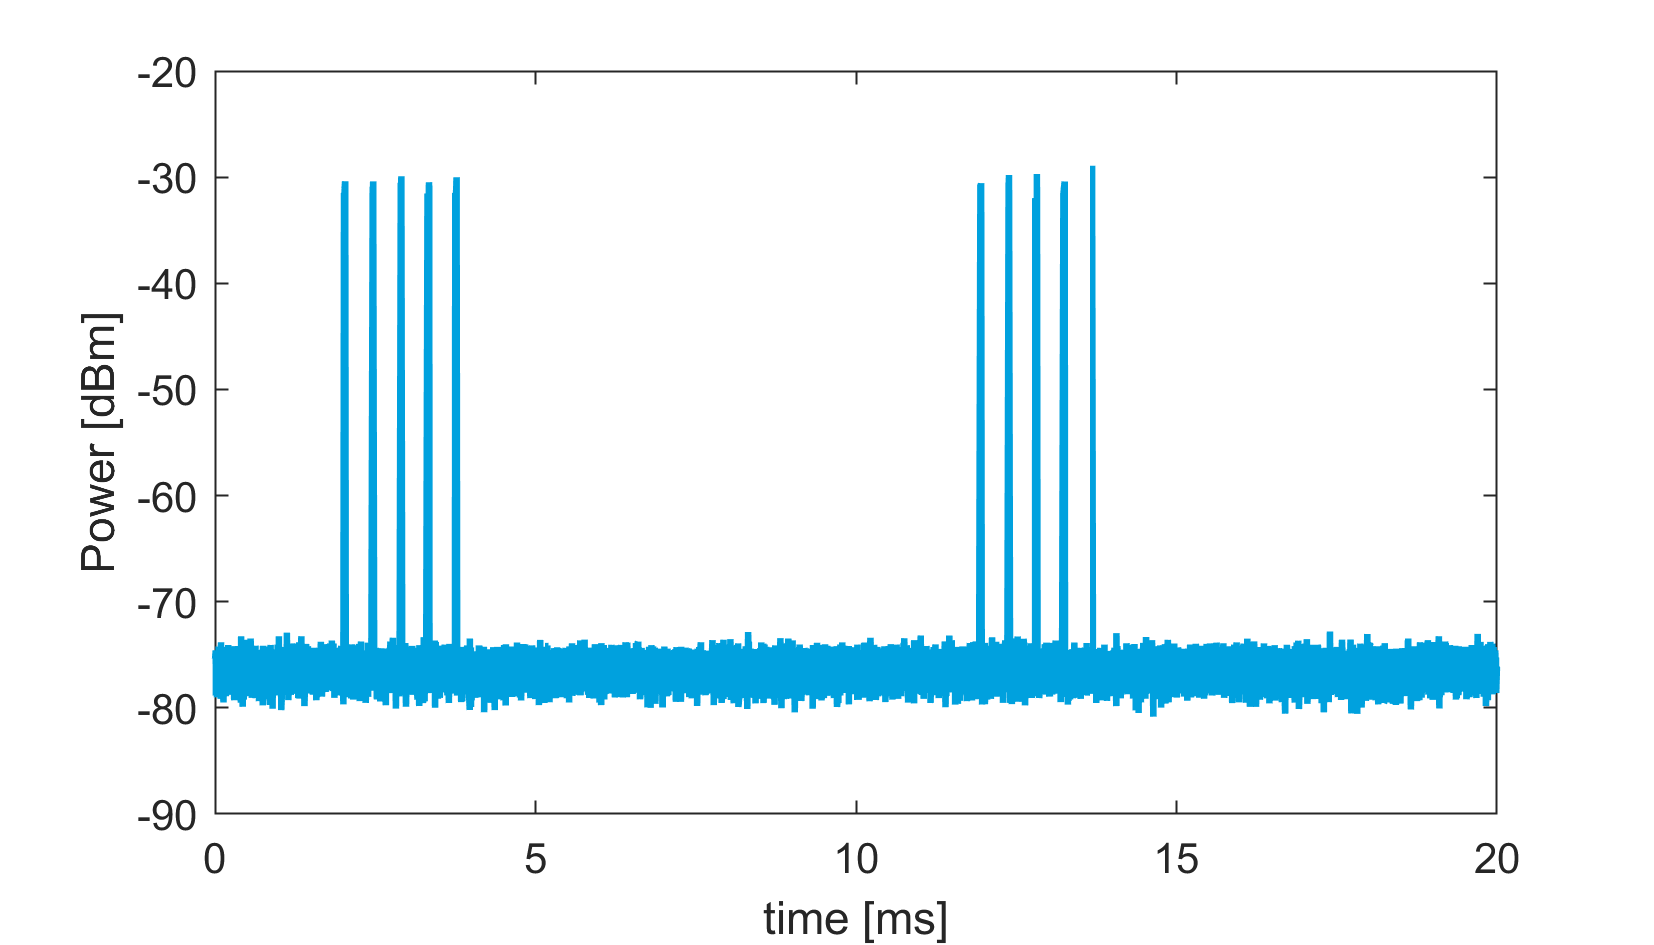
\includegraphics[width=0.49\textwidth]{trace_20.png}} \label{fig:n}
  \centering
  \subfigure[Zoomed trace of Figure (c)]{\includegraphics[width=0.49\textwidth]{{trace_20_zoom.png}}}
\caption{Trace}
\label{fig:rands}
\end{figure}



\subsection{Link Budget} \label{sec:lb}
The link-budget is necessary to design the complete end-to-end measurement system. Consider receiver blocking measurement and hence we require a blocking signal from the signal generator. Figure \ref{fig:link} explains the calculation of the levels within the system. \\

Suppose the calculated power (i.e. a maximum of an average of \acs{RMS} burst power) at the analyzer is -38~dBm, total attenuation (switching modules and cables) is 25~dB and maximum \acs{EIRP} is 15~dBm. Then, by using the formula from the previous section \ref{eq:bl}, the coupling loss at ANT 5 is 28~dB. According to the standard, receiver blocking measurement requires a blocker level of -47~dBm in front of the \acs{DUT} port. Then, to find the value of the level at the generator, we need to calculate backward. Therefore the value at the generator would be given by equation \ref{eq:BL}.
\begin{equation}
\mbox{Blocker Level}_{\mbox{generator}}  = \mbox{Blocker Level}_{\mbox{DUT}} + \mbox{Attenuation}_{\mbox{total}} + \mbox{Coupling Loss} \label{eq:BL}
\end{equation}
Antenna Gain is already taken care of since the standard defined the power levels in front of the \acs{DUT} Antenna. Assume that the attenuation for this path is 18~dB. Therefore, by using the above formula, the power at the generator is 1~dBm. Attenuations are frequency-dependent and for the coupling loss, we can only rely on the used frequencies of the \acs{DUT}. Nevertheless, for the paths within the switching modules and the cables, the available calibration data for the specific frequency is used. As the blocker frequencies are not too far away (Figure \ref{fig:ax} ) from the in-band frequencies, the same coupling loss is considered.

\begin{figure}[H]
%\centering
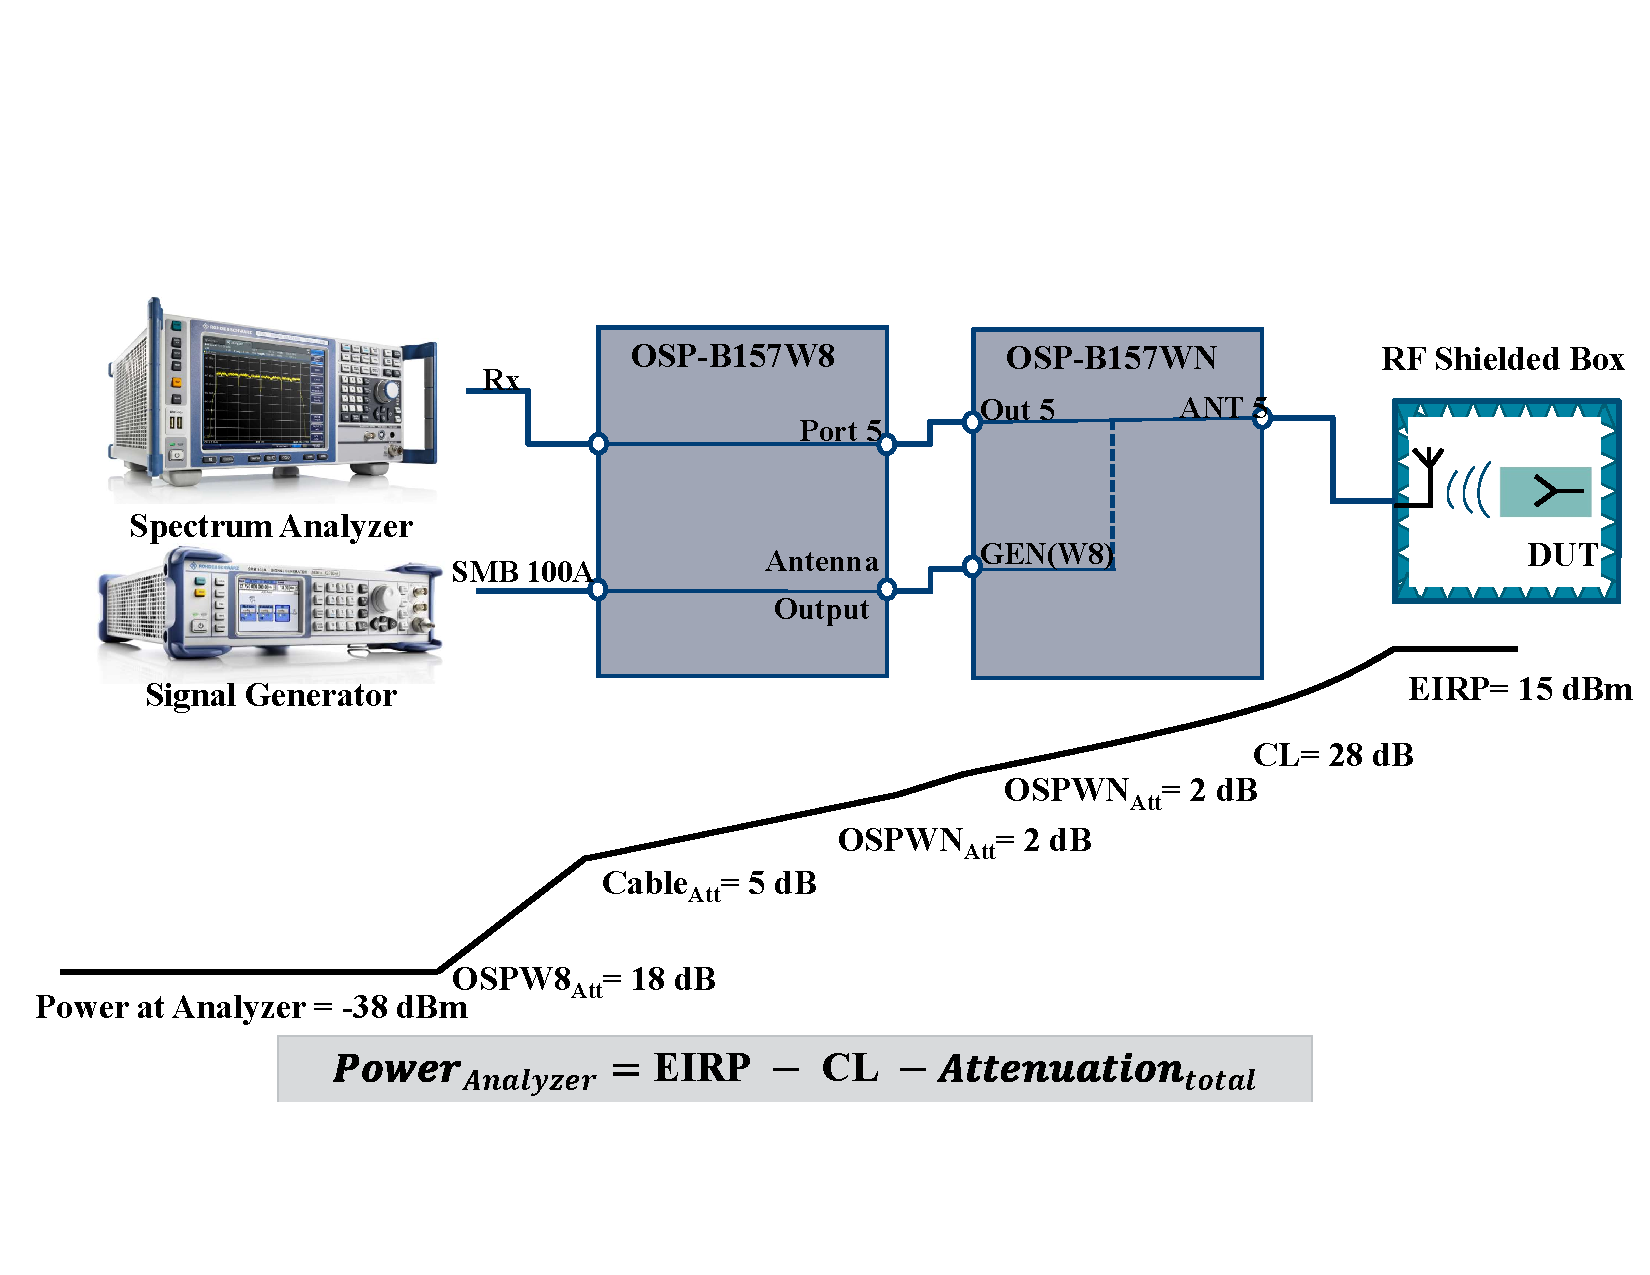
\includegraphics[scale = 0.57]{link_budget.pdf}\vspace{-1.6cm}
\caption{Link Budget diagram}
\label{fig:link} 
\end{figure}



\section{Optimization of Antenna Pair} \label{sec:opti}
Optimization of the probe antenna pairs is essential to ensure that the measurements are realized in optimal connections configurations with minimal losses and cabling again is not intended. The best selection of antenna pair is first implemented by performing a simulation on MATLAB\textregistered{} and later checking if the result coincides with the result from actual measurements. The later is also performed using the same algorithm. An important aspect to remember is that, as it is seen from the internal circuit diagram of OSPWN (\ref{fig:ospwn}) the antennas are arranged in pairs. And therefore, there are 15 possibilities for the optimum antenna pair selection.

\subsection{Simulation} 
To correctly perform the \acs{OTA} measurements in the \acs{RF} shielded box, a simulation for the link-budget analysis inside of the test chamber is required. This simulation, which is developed in MATLAB\textregistered{} environment will enable the choice of the best combinations of probe antenna pairs. For this purpose, a simulation of the transmission between the \acs{DUT} and all of the 6 probe antennas within the chamber, will allow a decision on the best associations between the instruments used for every test-case/measurement. The simulation also visualizes the effect of the positioning of a single-antenna \acs{DUT} within the chamber. The following parameters are considered in the simulation.
\begin{itemize}
  \item Configuration: The parameters of the chamber in the simulation e.g. the dimension of the chamber, antennas and, grid which holds the \acs{DUT}, placement of the antennas are tried to meet the existing system (Figure \ref{fig:room}). 
  \begin{figure}[H]
%\centering
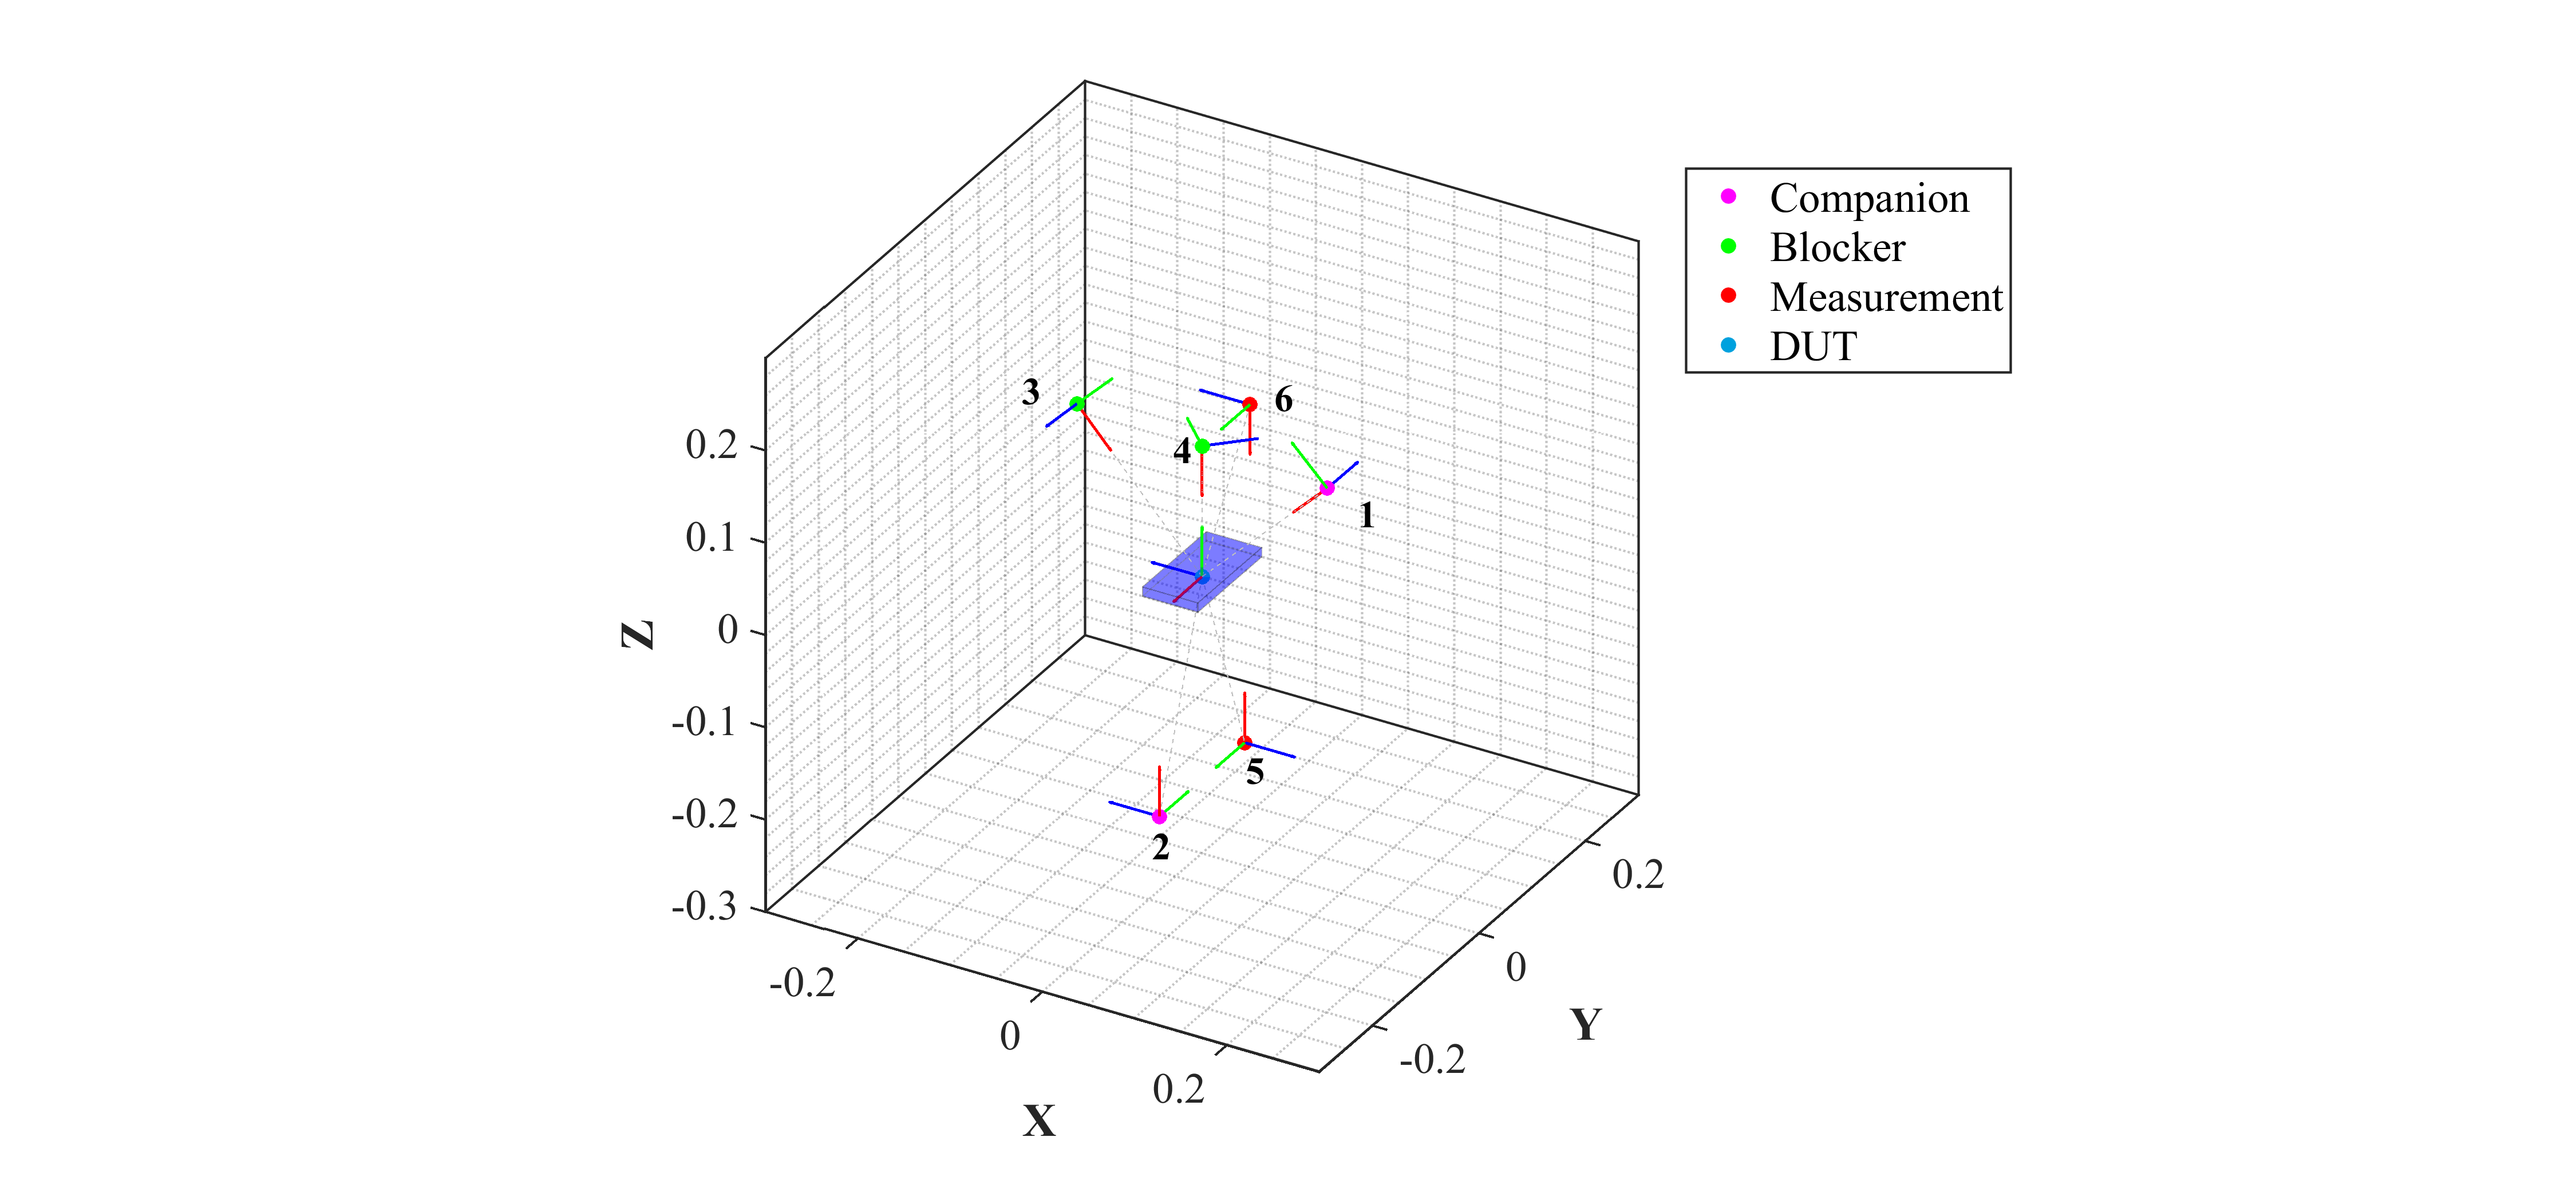
\includegraphics[scale = 0.45]{room.png}
\caption{Simulation diagram for the \acs{RF} shielded box}
\label{fig:room} 
\end{figure}

  \item \acf{FSPL}: This loss, which is given by the \acf{NF} formula for path loss \cite{schantz}, is caused because of the distance separating the antennas and the frequency of the \acs{DUT} (2412 MHz). The \acs{NF} model used is not very accurate and therefore can result in wrong solutions. Theoretically, we are not supposed to perform measurements in \acf{NF} but since for we only have single-antenna pair in this case and we don't bother about the phase offset and phase curvature of the signal, the measurements are possible. Incase of multi-antenna \acsp{DUT} with antenna arrays, this is theoretically not possible due to the large antenna size resulting to perform measurements in the far-field. The test system is officially proposed for the use of single-antenna \acsp{DUT}. Nevertheless, we performed the tests with multi-antenna \acs{DUT} to examine if the theoretical effects play an important role.
 
  \item Antenna Polarization Loss: The polarization loss is due to the difference in positioning the antennas that directly influences the results of the choice of the best probe antenna pairs. We use the theory (section \ref{sec:pol}) and the MATLAB\textregistered{} functions to first compute the electromagnetic fields of each transmitter and receiver antenna in its local coordinates system based on their positions and types, then we find the horizontal and vertical components of the electric fields, which are needed for the MATLAB\textregistered{} function \textit{pollos} to compute the polarization loss between each two antennas (refer coordinates system \ref{pollos}).
  
  \item Antenna Gain (Transmitter gain ($\mbox{G}_{\mbox{TX}}$) and Receiver Gain ($\mbox{G}_{\mbox{RX}}$): For each used antenna, we compute and save its antenna pattern. Radiation patter for the vivaldi (probe) as well as dipole (\acs{DUT}) antenna is used from the MATLAB\textregistered{} antenna toolbox. Therefore the values are not exactly the same as the actual antennas used in the experimental setup. For the configuration for the room, we can locate a transmitter's coordinates in the local's coordinates system of the receiver and vice versa, so that from the look up table of the gain, we can use the local coordinates to find the gain of both the \acs{DUT} and the considered probe antenna. These values for the gain are added in the final formula  (\ref{eq:pl}) to compute the final loss between each probe antenna and the \acs{DUT}.
  
  \item Total Path Loss:
  The total path loss is given by the formula \ref{eq:pl},
  \begin{equation}  \label{eq:pl}
  \begin{split}
  \mbox{Path Loss (k,r)}  & = \mbox{FSPL} - \mbox{Antenna Gains} + \mbox{Polarization Loss} \\
  &= 10 \log\frac{4}{\frac{1}{(kr)^6}-\frac{1}{(kr)^4}+\frac{1}{(kr)^2}} - \mbox{G}_{\mbox{TX}} - \mbox{G}_{\mbox{RX}} + \mbox{Polarization Loss}
 \end{split}
 \end{equation}
   
   \end{itemize}
   
   
The simulation runs over 4000 random positions of the \acs{DUT} on the grid (\ref{fig:try}) inside of the chamber with randomly one of the three different orientation of its antenna as illustrated in the picture (link). For each position the total loss between the \acs{DUT} and each probe antenna is computed. Since for each instrument (Spectrum analyzer, companion or signal generator) a pair of probe antennas should be assigned for the connection, from which only one with the lowest path loss should be used for the measurement. Since we have 6 different probe antennas, and 3 instruments, there are 15 distinct different possibilities of combinations of 3 pairs of antennas, one pair for each instrument with one active probe antennas. From these 15 possibilities, the simulation allows a choice of the best combination with the lowest mean path loss, i.e. the mean of the minima of every 3 pairs out of the 15 is computed and then the best combination is found. Refer Figure \ref{fig:s} for the results from  15 antenna pair possibilities.

\begin{figure}[H]
\vspace{-3cm}
  \hspace{-1.7cm}
  \subfigure {\includegraphics[width=0.67\textwidth]{simulation_best.pdf}} 
  \hspace{-3cm}
 % \centering
  \subfigure{\includegraphics[width=0.67\textwidth]{simulation_worst.pdf}}
   \vspace{-4.8cm}
\caption{Figure in the left and right display the best and worst selection of probe antenna pairs after the simulation respectively}
\label{fig:simu}
\end{figure}



\subsection{Experimental Measurement} 
The small chamber in use is TS7124M which is a \acs{RF} shielding box with flat absorbers, which are used in order to minimize the effect of reflections. \acs{RF} shielded boxes are essential for reliably testing radio interfaces. The \acs{RS}\textregistered{} TS7124M \acs{RF} shielded boxes enable reliable and reproducible measurements when a shielded test environment is needed. \\

Normalization measurement is performed at 23 different positions (refer Figure \ref{fig:m}) inside the RF shielded box to find the range in which the coupling loss lies. The \acs{DUT} antenna is oriented in three different directions :horizontal, vertical and slant. Since the \acs{DUT} tray is small, it is enough to place the \acs{DUT} at 9 locations in horizontal and vertical orientation. And the remaining 5 locations are acquired when the \acs{DUT} antenna is in slant orientation. The limit of the coupling loss is defined by us and it states that the coupling loss must be less than 35~dB (refer \ref{eq:egBL}) so that an additional amplifier is not required in the hardware setup. For example, consider receiver blocking measurement. The equation \ref{eq:BL} explains the procedure to find the level of the blocking signal at the signal generator given the blocker level infront of the \acs{DUT}. Now, if the coupling loss is more than 35~dB (i.e 40~dB) then, the level at the blocker would be:
\begin{equation} 
\begin{split}
\mbox{Blocker Level}_{\mbox{generator}}  &= \mbox{Blocker Level}_{\mbox{DUT}} + \mbox{Attenuation}_{\mbox{total}} + \mbox{Coupling Loss} \label{eq:egBL} \\
& = -47 \mbox{~dBm} + 18 \mbox{~dB} + 40 \mbox{~dB} \\
& = 11 \mbox{~dBm} 
\end{split}
\end{equation}
Since we keep increasing the blocker level by steps of 1~dB from this value to check for 10\% \acs{PER}, the increase is usually around 15~dB from the value which is calculated (11~dBm). Thus, the limit of the level from the signal generator, which is +26~dBm will soon be reached. And therefore we would require additional amplifiers. In-order to not complicate the system by the use of additional amplifiers, the limit of 35~dB is set for the coupling loss. The figure \ref{fig:man} shows that Antenna 1 and 6, Antenna 2 and 3 and Antenna 4 and 5 result in minimum mean coupling loss as well as almost all bins as seen in the plot are below 35~dB of coupling loss. The remaining plots from the possible combinations are in Figure \ref{fig:n}.

\begin{figure}[H]
  \subfigure {\includegraphics[width=0.5\textwidth]{manual_best.png}} 
  \subfigure{\includegraphics[width=0.5\textwidth]{manual_worst.png}}
\caption{Figure in the left and right display the best and worst selection of probe antenna pairs after the actual measurement respectively}
\label{fig:man}
\end{figure}

Comparing the simulation to the actual measurement, it can be noted that the range in which the coupling loss lies is approximately the same. Unfortunately the optimum pair does not match with pair resulting from the actual measurement. This can have several reasons: 
\begin{itemize}
\item Simulations take no charge of the reflections within the chamber. At some points in the chamber, there can be constructive or destructive interference. This increases the standard deviation because at some points we will see less power than simulations and at other we will see more power. These reflections can be due to the antenna mounting/holder and housing of the chamber. Because of the small size and flat absorbers of the \acs{RF} shielded box, the shielded box does not allow good anechoic performance.
\item The radiation pattern of the actual antennas might be different from the simulated antennas. This is because, simulation considered the radiation pattern from the MATLAB\textregistered{} antenna toolbox and not the actual used probe antennas which are manufactured at \acs{RS}\textregistered{}. In reality it can also happen that one probe antenna is 2~dB worse than the others. 
\item The antenna pattern which is used is the pattern from \acf{FF} measurements and therefore the pattern in \acf{NF} may look very different
\item The \acf{NF} model which is used to find the formula for \acf{FSPL} might be inaccurate.
\item Due to the small size and flat absorbers of the RF shielded box, it does not allow good anechoic performance.
\end{itemize}



\section{Selection of Best Probe Antenna} \label{sec:sba}
The selection of the best probe antenna for each device depends on the coupling loss and the measurement test case. Isolation between the used probe antennas could be an additional parameter that may be important but this thesis does not consider it. Receiver blocking requires a signal generator and a companion device. The companion device is connected to COMP1 of the switching module OSPWN (refer Figure \ref{fig:ospwn}) and hence only antenna 1 and antenna 2 can be used for the companion device. The one with lower coupling loss would be considered as the best probe antenna. For the signal generator, only antenna 5 and 6 can be used since these paths go to GEN W(8) of the OSPWN. Again the one with less coupling loss will be the best probe antenna. Similarly, \acf{OBW} and \acf{PSD} measurements require a companion device and the spectrum analyzer. The best probe antenna is selected for the companion device from antenna 1 and antenna 2. The analyzer can then use any of the five remaining antennas.




















\chapter{Data Evaluation}\label{chap:de}
This chapter is a consequence of the conducted and normalized measurements performed using a single-antenna \acs{DUT} and a multi-antenna \acs{DUT}. Each test is run for many times in-order to assess the \acf{MU}. 

\section{Measurement Analysis}
This section is sub-divided into two other sections: first when the \acs{DUT} is assessed for its transmitter capabilities and second for measurement of \acs{DUT} for its receiver capabilities. This sections also explains the reasons for using the fritz box as a companion device for \acs{PSD} measurement and for using some different spectrum analyzer settings from the settings mentioned by the standard.


\subsection{\acs{DUT} assessment for transmitter capabilities} 
The procedure for the \acf{OBW} measurement and \acf{PSD} are explained in detail in chapter \ref{chap:test}. Figure \ref{fig:nt} depicts the measurement when the \acs{DUT} sends echo packets and is checked for is transmitter capabilities. The spectrum analyzer saves the traces so that we can measure the bandwidth and the \acf{PSD} of the signal from the \acs{DUT}. When using a fritz box (section \ref{sec:golden}) as a companion device, data is transmitted and not just \acs{ICMP} packets.


\begin{figure}[H]
\centering
\includegraphics[scale = 0.46]{normalized_dut_transmitter.pdf}
\vspace{-1.3cm}
\caption{Normalized measurement of \acs{DUT} assessed for its transmitter capabilities}
\label{fig:nt} 
\end{figure}

Attenuation in the signal analyzer settings is kept to 10~dB and the pre-amplification is switched-off for conducted measurements because of the need of the signal to have a  high dynamic-range, i.e. to make sure that the power envelope is sufficiently above the noise floor of the analyser and to avoid the noise signals left and right from the power envelope being taken into account by this measurement. But, during radiated measurements, the pre-amplification is switched-on and the attenuation is brought down to 0~dB. This is because if the same conducted measurement settings are applied to radiated measurements, the dynamic-range and the noise floor of the signal is low which therefore increases the bandwidth of the signal (Figure \ref{fig:o}). 

\begin{figure}[H]
  \centering
  \subfigure[Bandwidth measurement with proper analyzer settings]{\includegraphics[width=0.49\textwidth]{OCBW_OTA_ATT0.png}} 
  \centering
  \subfigure[Low dynamic range of the system causing increase in bandwidth]{\includegraphics[width=0.49\textwidth]{{OCBW_OTA_ATT10.png}}} 
\caption{Increase in bandwidth of the signal due to low dynamic range}
\label{fig:o}
\end{figure}

The settings for the analyzer mentioned above also applies to \acf{PSD} measurement. In-addition to that, after running the \acs{PSD} measurement only for few times, there is a difference in the result every single time. This can be clearly seen from Figure \ref{fig:psdpsd}. The maximum value is 8.64~dBm and minimum is 7.12~dBm and hence there difference between the two is around 1~dBm which does not look very good. \acf{MU} is high due to low duty-cycle of the signal from \acf{CMW} due to \acs{ICMP} packets. The \acf{MU} is high for low duty-cycle signals because when we use \acs{RMS} detector and Max-Hold over all traces, it means if the burst is very short, it would be maximum only when the measurement time for that particular frequency is aligned with the burst.  If suppose it is shifted by 50\% then the values would be 3dB lower. This means it will take forever to stabilize this measurement. Measurement works better with high duty-cycle signals. Therefore, fritz box is used as a companion device for this measurement instead of the connectivity tester.
\begin{figure}[H]
\centering
\includegraphics[scale = 0.85]{PSD_trace_differnce.png}
\caption{\acf{MU} in the \acs{PSD} measurement caused due to low duty cycle of the signal}
\label{fig:psdpsd} 
\end{figure}



\subsection{\acs{DUT} assessment for receiver capabilities}
Figure \ref{fig:nr} pictures the measurement of \acs{DUT} for its receiver ability. This is achieved by using \acf{PER} measurement (section \ref{sec:rxmeas}).

\begin{figure}[H]
\centering
\includegraphics[scale = 0.46]{normalized_dut_receiver.pdf}
\vspace{-1.3cm}
\caption{Normalized measurement of \acs{DUT} assessed for its receiver capabilities}
\label{fig:nr} 
\end{figure}

The spectrum analyzer shows the DUT signal and the blocking signal. It can be seen that the signal from the blocker is not very far from the in-band frequency of the \acs{DUT}.
\begin{figure}[H]
\centering
\includegraphics[scale = 0.24]{analyzer_rx.PNG}
\caption{Trace on the spectrum analyzer \acs{GUI}}
\label{fig:ax} 
\end{figure}


\section{\acf{MU}}
\acf{MU} is evaluated by running each test case (i.e. \acf{OBW}, \acf{PSD}, and Receiver Blocking) several times and then comparing the results (i.e. standard deviation and mean) of conducted and normalized measurements. Computation of \acs{MU} is done using two \acsp{DUT} (i.e. single-antenna \acs{DUT} and multi-antenna \acs{DUT}). Since the multi-antenna \acs{DUT} does not have a cable connector, we do the measurements only radiated (i.e normalized) and comparing it with conducted is not possible. \\

For the \acs{PSD} and Receiver Blocking measurement, the calculation of mean is done by converting the power level from dBm scale to linear scale because it is physically correct to use mean from the linear scale. The standard deviation is calculated by using the power values in dBm scale. 

\subsection{Single-Antenna \acs{DUT}}
This section gathers the information of \acf{MU} for each test case for both conducted and normalized type. The following reveals the results of the long-term measurements.

\subsubsection{\acf{OBW} Measurement}
The \acs{OBW} test is run 300 times for each conducted and normalized type of measurement. Figure \ref{fig:otavscond} potrays the result from the long-term measurements.

\begin{figure}[H]
\centering
\subfigure[Conducted measurement]{\includegraphics[scale=0.55]{bandwidth_conducted_single_300.PNG}} 
\subfigure[Normalized measurement]{\includegraphics[scale = 0.55]{bandwidth_OTA_single_300.PNG}}  
\caption{Histogram of \acs{OBW} test-case resulting from 300 measurements }
\label{fig:otavscond} 
\end{figure}

From the plots it is clear that the \acf{MU} is almost equal in both conducted and normalized type of measurements. The table \ref{tab:tab1} arranges the results from the Figure \ref{fig:otavscond} to a tabular form. 

\begin{table}[H]
  \centering
\begin {tabular} {|c|c|c|} 
\toprule
 & \textbf{Conducted Measurement} & \textbf{Normalized Measurement} \\ 
\midrule 
\textbf{Mean} & 16.43~MHz & 16.42~MHz\\
\textbf{Standard Deviation} & 0.01~MHz & 0.01~MHz\\
\bottomrule
 \end{tabular}
  \caption{\acf{MU} results for \acs{OBW} measurement} \label{tab:tab1}
\end{table}

\subsubsection{\acf{PSD} Measurement}
The \acs{PSD} measurement is run 60 times for each conducted and normalzed type of measurement. Figure
\ref{fig:otavscond2} shows the result from the long-term measurement.
\begin{figure}[H]
\centering
\subfigure[Conducted measurement]{\includegraphics[scale=0.55]{PSD_conducted_single_60.PNG}}
\subfigure[Normalized measurement]{\includegraphics[scale = 0.55]{PSD_OTA_single_60.PNG}}
\caption{Histogram of \acs{PSD} test-case resulting from 60 measurements }
\label{fig:otavscond2} 
\end{figure}
It is comprehensible from the figure \ref{fig:otavscond2} as well as the table \ref{tab:tab2} that the results achieved by using conducted measurements have lower \acs{MU} compared to the ones using normalized measurements.
\begin{table}[H]
  \centering
\begin {tabular} {|c|c|c|} 
\toprule
 & \textbf{Conducted Measurement} & \textbf{Normalized Measurement} \\ 
\midrule 
\textbf{Mean} & 3.15~dBm/MHz & 3.03~dBm/MHz\\
\textbf{Standard Deviation} & 0.08~dBm/MHz & 0.18~dBm/MHz\\
\bottomrule
 \end{tabular}
  \caption{\acf{MU} results for \acs{PSD} measurement} \label{tab:tab2}
\end{table}


\subsubsection{Receiver Blocking Measurement}
The Receiver Blocking measurement is run 60 times for each conducted and normalized type of measurement. Figure \ref{fig:otavscond3} presents the occurrence of the blocker level which results in 10\% PER at each frequency in a long-term measurement.
\begin{figure}[H]
\centering
\subfigure[Conducted measurement]{\includegraphics[scale=0.55]{RxBlocking_conducted_singleAntenna_2300_60.PNG}}
\subfigure[Normalized measurement]{\includegraphics[scale=0.55]{RxBlocking2300.PNG}} \\
\subfigure[Conducted measurement]{\includegraphics[scale=0.55]{RxBlocking_conducted_singleAntenna_2330.PNG}}
\subfigure[Normalized measurement]{\includegraphics[scale=0.55]{RxBlocking2330.PNG}} \\
\subfigure[Conducted measurement]{\includegraphics[scale=0.55]{RxBlocking_conducted_singleAntenna_2360.PNG}}
\subfigure[Normalized measurement]{\includegraphics[scale=0.55]{RxBlocking2360.PNG}} \\
\subfigure[Conducted measurement]{\includegraphics[scale=0.55]{RxBlocking_conducted_singleAntenna_2380.PNG}}
\subfigure[Normalized measurement]{\includegraphics[scale=0.55]{RxBlocking2380.PNG}} \\
\caption{Histogram of Receiver Blocking test-case resulting from 60 measurements }
\label{fig:otavscond3} 
\end{figure}

Also in this test-case, the conducted measurement results appear to have lower \acs{MU}. In all the three test-cases, the measurement results by normalized measurements are close to the ones performed by performing the measurements in a conducted way.
\begin{table}[H]
\resizebox{\textwidth}{!}
{
        \begin{tabular}{|c|c|c|c|}\toprule
         \textbf{Blocker Frequency} & \textbf{MU Parameters} &\textbf{Conducted Measurement} & \textbf{Normalized Measurement} \\
            \midrule
            \textbf{2300 MHz} & Mean                      & -36.63~dBm & -36.71~dBm \\
                             & Standard Deviation & 0.08~dBm    & 0.13~dBm  \\
                             \midrule
            \textbf{2330 MHz} & Mean                      & -37.54~dBm & -37.52~dBm       \\
                             & Standard Deviation & 0.09~dBm    & 0.16~dBm       \\
                             \midrule
            \textbf{2360 MHz} & Mean                      & -39.15~dBm & -39.10~dBm     \\
                             & Standard Deviation & 0.06~dBm    & 0.13~dBm      \\
                             \midrule
            \textbf{2380 MHz} & Mean                      & -49.82~dBm & -49.73~dBm       \\
                             & Standard Deviation & 0.09~dBm    & 0.18~dBm \\
           \bottomrule
        \end{tabular}}
        \caption{\acf{MU} results for Receiver Blocking measurement}\label{tab:Tab3}
 \end{table} 




\subsection{Multi-Antenna \acs{DUT}}
The same three measurements are performed using multi-antenna \acs{DUT}. The measurements are run for the same number of times as the previously depicted single-antenna \acs{DUT}. Table \ref{tab:Tab4} lays out the results for mean and standard deviation from the test-cases.
\begin{table}[H]
\resizebox{\textwidth}{!}
{
        \begin{tabular}{|c|c|c|c|}\toprule
         \textbf{Test-Case} & Parameters & \textbf{MU Parameters} & \textbf{Normalized Measurement} \\
            \midrule
           Receiver Blocking & Blocker level at 2300 MHz & Mean     & -33.03 dBm \\
                         &    & Standard Deviation & 0.14 dBm     \\

          &  Blocker level at 2330 MHz & Mean     & -31.16 dBm       \\
                     &        & Standard Deviation & 0.12 dBm    \\

          & Blocker level at 2360 MHz & Mean       & -29.01 dBm    \\
                          &   & Standard Deviation & 0.13 dBm      \\
                           
          & Blocker level at 2380 MHz & Mean      & -35.64 dBm    \\
                       &      & Standard Deviation & 0.09 dBm     \\
                       \midrule
                      
          Occupied Channel Bandwidth & 99\% bandwidth & Mean & 16.50 MHz \\
           &  & Standard Deviation & 0.02 MHz \\
           
           \midrule
           Power Spectral Density &   maximum (mean(EIRP)) & Mean &  3.20 dBm/MHz \\
           & & Standard Deviation & 0.11 dBm/MHz \\          
           \bottomrule
        \end{tabular}}
        \caption{\acf{MU} results for measurements using Multi-Antenna \acs{DUT}}\label{tab:Tab4}
 \end{table} 

The specification sheet of this \acs{DUT} mentions that the device uses diversity to primarily to improve performance over a fading radio channel. In such a system, the receiver is provided with multiple copies of the same information signal which are transmitted over two or more real or virtual communication channels. Thus the basic idea of diversity is repetition or redundancy of information. In virtually all the applications, the diversity decisions are made by the receiver and are unknown to the transmitter. \\

\begin{figure}[H]
\centering
\includegraphics[scale = 0.85]{Beamforming_all_new.PNG}
\caption{Investigating diversity performance of the \acs{DUT}}
\label{fig:11} 
\end{figure}

To prove that the \acs{DUT} does-not perform diversity when assessed for its transmitter capabilities, a long-term power measurement to calculate the coupling loss (refer section \ref{sec:11}) is done. Measurements were performed after with random time gaps between the two measurements to investigate if the results differ due to beam-forming. The Figure \ref{fig:11} shows the result of coupling loss for 70 measurements with random time-gap. The companion device is first connected to ANT 1 port of the switching module (OSP-B157WN) and then the coupling loss is found at other antenna ports. In the next step, the companion device is connected to ANT 2 port and the coupling loss is again found at all the other ports. If diversity was done when the \acs{DUT} is assessed for its transmitter capability, the antenna pattern would change when connecting the companion device to port ANT 2. Since it is not the case as seen from the Figure \ref{fig:op}, we know that diversity is applicable only for receiver measurements.










\chapter{Conclusion} \label{chap:8}

The achieved findings of this work shall be described in this chapter. Furthermore, an outlook for future work will be drawn.

\section{Achievements}
This work presents a coexistence testing solution for devices with or without antenna ports, based on a novel regulatory test system that has a compact size and high quality shielding and allows lower coupling losses. The project implements normalized and conducted measurements to perform the device-testing, and investigates the MU for both cases. To this end, an algorithm for the optimization of antenna pairs is implemented on both the simulation and the measurements. After that, the hardware and software implementations for PSD and receiver blocking test cases are done based on the standard (link). The results for both single and multi-antennas DUTs showed that comparable MU results to the conducted measurements can be achieved by the normalized approach. While studying the MU results for the presented test cases, many factors may influence the accuracy of the test results. In addition to the errors caused by thermal noise, there are interferences and cross-talk between the measurement antennas that can influence the results. Also, the results of the MU for single-antennas DUT are proved to be better than those of multi-antennas. Finally, in-band testing determines the performance of wireless devices and the thresholds where wireless communications are degraded as well as the threshold where communications stop i.e where the limits set by the standards are exceeded. The report of these tests provides the necessary data to make a more informed risk analysis of the radio?s behavior and to enable troubleshooting the reported interference problems. The results prove that performing the normalized OTA measurements doesn?t result in a major degrading the quality of the evaluation.
Further investigations and research are possible to improve this work; for the selection of best probe antennas within the test chamber, the simulation can be improved by including other effects that can increase the accuracy of the simulation to match the choice based on actual measurements such as minor reflections in the chamber and isolation between the probe antennas (link).


\section{Outlook}


\printbibliography
%%%%%%%%%%%%%%%%%%%%%%%%%%%%%%%%%%%%%%%5



\chapter{Annex}

This appendix gathers the measurement results of the main scenarios investigated
for the thesis. 

\begin{figure}[H]
     \subfigure{\includegraphics[scale = 0.37]{/Annex/Manual/plot1.png}} 
     \subfigure{\includegraphics[scale = 0.37]{/Annex/Manual/plot2.png}} 
     \subfigure{\includegraphics[scale = 0.37]{/Annex/Manual/plot3.png}}  \\
     \subfigure{\includegraphics[scale = 0.37]{/Annex/Manual/plot4.png}} 
     \subfigure{\includegraphics[scale = 0.37]{/Annex/Manual/plot5.png}} 
     \subfigure{\includegraphics[scale = 0.37]{/Annex/Manual/plot6.png}}  \\
     \subfigure{\includegraphics[scale = 0.37]{/Annex/Manual/plot7.png}} 
     \subfigure{\includegraphics[scale = 0.37]{/Annex/Manual/plot8.png}} 
     \subfigure{\includegraphics[scale = 0.37]{/Annex/Manual/plot9.png}}  \\
     \subfigure{\includegraphics[scale = 0.37]{/Annex/Manual/plot10.png}} 
     \subfigure{\includegraphics[scale = 0.37]{/Annex/Manual/plot11.png}} 
     \subfigure{\includegraphics[scale = 0.37]{/Annex/Manual/plot12.png}}  \\
      \subfigure{\includegraphics[scale = 0.37]{/Annex/Manual/plot13.png}} 
     \subfigure{\includegraphics[scale = 0.37]{/Annex/Manual/plot14.png}} 
     \subfigure{\includegraphics[scale = 0.37]{/Annex/Manual/plot15.png}}  
        \caption{Manual Measurements for optimization of antenna pair}
        \label{fig:three graphs}
\end{figure}






\begin{singlespace}




\end{singlespace}
\end{document}
